\documentclass[a4paper]{report}
\usepackage{lipsum}
\usepackage{tikzpagenodes}
\usepackage{pgfplots}
\usepackage{tikz}
\usepackage{tikz-3dplot}
\usetikzlibrary{arrows,decorations.pathmorphing,backgrounds,positioning,fit,matrix}
\pgfplotsset{compat=1.8}
\usepackage{graphics} % for pdf, bitmapped graphics files
\usepackage{epsfig} % for postscript graphics files
\usepackage[colorlinks=true,citecolor=green]{hyperref}
\usepackage{cite}
\usepackage{amsmath,amssymb,amsfonts}
\usepackage{algorithmic}
\usepackage{graphicx}
\usepackage{url}
\usepackage{cite}
\usepackage{bm}
\usepackage{pbox}
\usepackage{siunitx,booktabs,etoolbox}
\usepackage{ulem}

\def\BibTeX{{\rm B\kern-.05em{\sc i\kern-.025em b}\kern-.08em
    T\kern-.1667em\lower.7ex\hbox{E}\kern-.125emX}}

\begin{document}
\chapter{TODO}
\section{TODO Pure hand eye solver}
TODO list:
pure solution:
\begin{enumerate}
	\item \sout{The dual quaternion solution};
	\item \sout{Dual quaternion based SOCP solution: trick};
	\item \sout{global polynomial optimization method};
	\item \sout{stochastic SE3 optimization;}
	\item \sout{SCF solution for quaternion and Kronecker};
	\item \sout{SE3 Gauss-Newton};
	\item \sout{benchmark test on ETH-ASL and MIT-RGB dataset};
	\item \sout{benchmark test};
	\item \sout{paper writing};
\end{enumerate}
Note: 
\begin{itemize}
\item \textcolor{blue}{small motion: like relative rotation is small. This is one of the most difficult cases.};
\item git\textcolor{blue}{SCF is not comparable to SQP, so I re-modify the formulation to a SDP problem and then solve with SDR and randomization. The performance is more stable.}
\end{itemize}

\section{TODO Vision}
TODO list:
pure solution:
\begin{enumerate}
	\item \sout{main entry};
	\item \sout{Feature tracker};
	\item \sout{Homography estimation in C++};
	\item \sout{Generalized RANSAC solver in C++};
	\item \sout{homography decompsition in matlab and using opencv};
	\item \sout{Feature detection \& matching with ORB};
	\item \sout{Naive matching outlier removal};
	\item \sout{$5$ point Essential and $8$ point fundamental estimation};
	\item \sout{Motion Estimation, 2d-2d,3d-2d,3d-3d};
	\item Refine;
	\item paper writing;
\end{enumerate}

\section{TODO KDTree}
TODO list:
\begin{enumerate}
\item Iterative closet point using nanoflann;
\end{enumerate}

\section{TODO time synchronization}
can we use TLBO or PSO to find the optimum t???


\chapter{$AX=XB$}
\section{Aims}

\begin{figure}
\centering
\tdplotsetmaincoords{60}{110}
%start tikz picture, and use the tdplot_main_coords style to implement the display 
%coordinate transformation provided by 3dplot
\begin{tikzpicture}[scale=3,tdplot_main_coords]
%-----------------------
\coordinate (A) at  (0,0,0);
\coordinate (Ax) at (0.5,0,0);
\coordinate (Ay) at (0,0.5,0);
\coordinate (Az) at (0,0,0.5);

\coordinate (A1) at  (-0.187,-0.504,-0.396);
\coordinate (A1x) at (0.255,-0.734,-0.189);
\coordinate (A1y) at (-0.107,-0.371,-0.673);
\coordinate (A1z) at (0.032,-0.083,-0.0432);

\coordinate (A2) at  (0,0,0);
\coordinate (A2x) at (0.5,0,0);
\coordinate (A2y) at (0,0.5,0);
\coordinate (A2z) at (0,0,0.5);


\coordinate (B) at  (0,1,-0.5);
\coordinate (Bx) at (0.5,1,-0.5);
\coordinate (By) at (0.0,1-0.5,-0.5);
\coordinate (Bz) at (0.0,1,-0);

\draw[-, line width=1mm, solid] (A) to[] node[left,rotate=0] {} (B);

%determine a coordinate (P) using (r,\theta,\phi) coordinates.  This command
%also determines (Pxy), (Pxz), and (Pyz): the xy-, xz-, and yz-projections
%of the point (P).
%syntax: \tdplotsetcoord{Coordinate name without parentheses}{r}{\theta}{\phi}
%\tdplotsetcoord{P}{\rvec}{\thetavec}{\phivec}
\coordinate (Shift) at (0.,0.,0.);
\tdplotsetrotatedcoords{-200}{90}{0}
\tdplotsetrotatedcoordsorigin{(Shift)}
%%%% draw A1
\draw[thick,color=green,tdplot_rotated_coords,->] (A) --
(Ax) node[anchor=north]{$y$};
\draw[thick,color=red,tdplot_rotated_coords,->] (A) --
(Ay) node[anchor=west]{$x$};
\draw[thick,color=blue,tdplot_rotated_coords,->] (A) --
(Az) node[anchor=south]{$z$};
\node (O) [left] {$\bold{A}_1$};

\draw[thick,color=green,tdplot_rotated_coords,->] (A1) --
(A1x) node[anchor=north]{$y$};
\draw[thick,color=red,tdplot_rotated_coords,->] (A1) --
(A1y) node[anchor=west]{$x$};
\draw[thick,color=blue,tdplot_rotated_coords,->] (A1) --
(A1z) node[anchor=south]{$z$};

%%%% draw B1
\draw[thick,color=green,tdplot_rotated_coords,->] (B) --
(Bx) node[anchor=north]{$y$};
\draw[thick,color=red,tdplot_rotated_coords,->] (B) --
(By) node[anchor=south]{$x$};
\draw[thick,color=blue,tdplot_rotated_coords,->] (B) --
(Bz) node[anchor=south]{$z$};
\node (B) at (-0,0.7,-0.5) [right] {$\bold{B}_1$};

\coordinate (Shift) at (-0.7,1.0,0.1);
\tdplotsetrotatedcoords{-70}{70}{45}
\tdplotsetrotatedcoordsorigin{(Shift)}
\coordinate (A2) at (-0.7,1.0,0.1);
\coordinate (A2x) at (-0.7,1.5,0.1);
\coordinate (A2z) at (-1.3,1.0,0.1);
\coordinate (A2y) at (-0.7,1.0,-0.4);
\coordinate (B2) at  (-0.7,1.7,-0.4);
\coordinate (B2x) at (-0.7,1.7-0.5,-0.4);
\coordinate (B2y) at (-0.2,1.7,-0.4);
\coordinate (B2z) at (-0.7,1.7,-0.4+0.5);
\draw[thick,color=red,tdplot_rotated_coords,->] (A2) --
(A2x) node[anchor=north east]{${x}$};
\draw[thick,color=green,tdplot_rotated_coords,->] (A2) --
(A2y) node[anchor=west]{${y}$};
\draw[thick,color=blue,tdplot_rotated_coords,->] (A2) --
(A2z) node[anchor=south]{${z}$};
\draw[thick,color=red,tdplot_rotated_coords,->] (B2) --
(B2x) node[anchor=north east]{${x}$};
\draw[thick,color=green,tdplot_rotated_coords,->] (B2) --
(B2y) node[anchor=north]{${y}$};
\draw[thick,color=blue,tdplot_rotated_coords,->] (B2) --
(B2z) node[anchor=south]{${z}$};
\draw (A2) node[left] {$\bold{A}_2$};
\draw (B2) node[right] {$\bold{B}_2$};
\draw[-, line width=1mm, solid] (A2) to[] node[left,rotate=0] {} (B2);

\coordinate (m1) at (-0.7,2.,-0.2);
\coordinate (mi) at (-0.7,2.0,-0.4);

\draw[loosely dotted, color=black] (m1) -- (mi);

\coordinate (Shift) at (-0.7,2.0,-0.8);
\tdplotsetrotatedcoords{-130}{90}{0}
\tdplotsetrotatedcoordsorigin{(Shift)}
\draw[thick,color=green,tdplot_rotated_coords,->] (0,0,0) --
(-.3,0,0) node[anchor=north east]{$\bold{M}_{iy}$};
\draw[thick,color=blue,tdplot_rotated_coords,->] (0,0,0) --
(0,.3,0) node[anchor=north west]{$\bold{M}_{iz}$};
\draw[thick,color=red,tdplot_rotated_coords,->] (0,0,0) --
(0,0,-.3) node[anchor=south west]{$\bold{M}_{ix}$};
%
%\coordinate (Shift) at (0.5,1.3,0.);
%\tdplotsetrotatedcoords{-45}{90}{0}
%\tdplotsetrotatedcoordsorigin{(Shift)}
%\draw[thick,color=green,tdplot_rotated_coords,->] (0,0,0) --
%(-0.7,0,0) node[anchor=north west]{$\bold{G}_y$};
%\draw[thick,color=blue,tdplot_rotated_coords,->] (0,0,0) --
%(0,.7,0) node[anchor=west]{$\bold{G}_z$};
%\draw[thick,color=red,tdplot_rotated_coords,->] (0,0,0) --
%(0,0,-.7) node[anchor=south]{$\bold{G}_x$};
%
%\coordinate (G) at (0.5,1.3,0.);
%
%\draw (G) node[left] {$\bold{G}$};
%\draw (-0.7,2.0,-0.8) node[below] {$\bold{M}_i$};
%\draw (-0.7,2.0,0.1) node[left] {$\bold{M}_1$};
%
%
%\draw[<->, dashed] (-0.7,2.0,0.1) to[bend right=80] node[left,rotate=0] {} (O);
%\draw[<->, dashed] (-0.7,2.0,-0.8) to[bend right=80] node[left,rotate=0] {} (O);
%
%\draw[<->, loosely dotted] (-0.7,2.0,-0.8) to[bend right=20] node[left,rotate=0] {} (-0.7,2.0,0.1);
%\draw[<->, loosely dotted] (O) to[bend right=50] node[above,rotate=0] {} (G);
%\draw[<->, loosely dotted] (-0.7,2.0,-0.8) to[bend right=50] node[above,rotate=0] {} (G);
%\draw[<->, loosely dotted] (-0.7,2.0,0.1) to[bend right=50] node[left,rotate=0] {} (G);

\end{tikzpicture}
\caption{Coordinate Systems. Dashed connections are transformation matrices directly measured and dotted connections are transformation matrices to be optimized.}
\label{fig:frame}
\end{figure}

Hand-Eye Calibration is the simulataneous computation of two unknown spatial relationships in a circle of spatial relationships.

The hand-eye calibration problem first appeared and got its name from the robotics community, where a camera ("eye") was mounted on the gripper ("hand") of a robot. The cameras was calibrated using a calibration pattern. Then the unknown transformation from the robot coordinate system to the calibration pattern coordinate system as well as the transformation from the camera to the hand coordinate system need to be estimated simultaneously.

Overall, the so called hand-eye calibration means to solve 
\begin{equation}
\mathbf{AX=XB}
\end{equation} or 
\begin{align}
\mathbf{R}_x&=\mathbf{R}_A\mathbf{R}_x\mathbf{R}_B \\ 
\mathbf{t}_x&=\mathbf{R_A}\mathbf{t}_x+\mathbf{t_A}-\mathbf{R}_x\mathbf{t_B}
\end{align}

\section{useful links}
\cite{tum_hand_eye}.\\
\url{https://github.com/jhu-lcsr/handeye_calib_camodocal}\\
\url{https://github.com/amy-tabb/RWHEC-Tabb-AhmadYousef}: method is very easy, use ceres for optimziation (LevMar), cost is the Frobenius norm, initizalize with the identity matrix~\cite{tabb2017solving}.\\
A good overview~\cite{shah2012overview} and also \url{http://faculty.cooper.edu/mili/Calibration/index.html}: include some 3D-3D solutions (very old one), hand-eye, world-eye, etc.

\section{data set}
\url{https://github.com/utiasSTARS/certifiable-calibration}.\\ 
\url{http://www.cvl.isy.liu.se/en/research/datasets/gopro-imu-dataset/}.



\section{sol1}
This solution was the earliest proposed method by~\cite{shiu1989calibration}. This method needs 2 measurements to estimate the $\mathbf{X}$. 
\begin{enumerate}
\item estimate particular sols $\mathbf{R_{XP}}_1$ and $\mathbf{R_{XP}}_2$;
\item construct a linear equation $\mathbf{A}x=b$ to estimate $beta_1$ and $beta_2$;
\item compute $\mathbf{R}_{12}$;
\item form another linear equation to estimate $\mathbf{t}_{12}$
\end{enumerate}
Details can be found in~\cite{shiu1989calibration}: equations (37)-(39), (54)-(55), (47)-(48).

\cite{shiu1989calibration} were apparently the
first to attack the problem and to report a mathematical
solution. They proved by an algebraic approach that (2)
and (3) are both rank deficient, and so one needs to
make at least two robot movements in order to
determine Rx and tx. Their method, however,
generates more unknowns ‘than necessary. 

\section{sol2}
This solution is given in~\cite{tsai1989new}. At least two significantly different measurements are needed.
\begin{enumerate}
\item estimate $P_r$ by taking the Rodriguez transformation to get the rotation vector $\vec{r}$ and then let $\theta=|r|, \vec{n}=\frac{r}{\theta}, P_r=2sin(\frac{\theta}{2})\vec{r}$.
\item stacking measurements together:
	\begin{align*}
		\left[
		\begin{matrix}
			skew({P_{r1}}_1+{P_{r2}}_1) \\
			skew({P_{r1}}_2+{P_{r2}}_2) \\
			\vdots \\
			skew({P_{r1}}_N+{P_{r2}}_N) \\
		\end{matrix}
		\right]\bar{P}_{cg} = \left[
		\begin{matrix}
		{P_{r1}}_1-{P_{r2}}_1 \\
		{P_{r1}}_2-{P_{r2}}_2 \\
		\vdots \\
		{P_{r1}}_N-{P_{r2}}_N \\
		\end{matrix}
		\right]
	\end{align*}
\item solve for $\bar{P}_{cg}$ and $P_{cg}=\frac{2\bar{P}_{cg}}{\sqrt{1+|\bar{P}_{cg}|^2}}$ and then reconstruct $R_{cg}=(1-|P_{cg}|^2*0.5)\mathbf{I}+0.5(P_{cg}P_{cg}^T+\sqrt{4-|P_{cg}|^2}skew(P_{cg}))$.
\item stacking as follows:
	\begin{align*}
		\left[
		\begin{matrix}
			\mathbf{R}_{g1}-\mathbf{I} \\
			\mathbf{R}_{g2}-\mathbf{I} \\
			\vdots \\
			\mathbf{R}_{gN}-\mathbf{I} \\
		\end{matrix}
		\right]{T}_{cg} = \left[
		\begin{matrix}
		\mathbf{R}_{cg}T_{c1}-T_{g1} \\ 
		\mathbf{R}_{cg}T_{c2}-T_{g2} \\ 
		\vdots \\
		\mathbf{R}_{cg}T_{cN}-T_{gN} \\ 
		\end{matrix}
		\right]
	\end{align*}
	then solve for $T_{cg}$.
\end{enumerate}
Accurate if a batch of measurements are provided.

\section{sol3}
Solution based on the Euclidean Group~\cite{park1994robot}. The analytical solution for two measurements are given as
\begin{align}
A_1 X = X B_1 \nonumber \\
A_2 X = X B_2 \nonumber \\
\alpha_1 = log(A_1)^{\vee} \nonumber \\
\alpha_2 = log(A_2)^{\vee} \nonumber \\
\beta_1 = log(B_1)^{\vee} \nonumber \\
\beta_2 = log(B_2)^{\vee} \nonumber \\
R = \mathcal{A}\mathcal{B}^{-1} \\
\mathcal{A}=\left[ \alpha_1,\alpha_2, \alpha_1 \times \alpha_2 \right] \nonumber \\
\mathcal{B}=\left[ \beta_1,\beta_2, \beta_1 \times \beta_2 \right] \nonumber
\end{align}
$T$ can be solved using the normal equation. If there are more than two measurements, a least square solution is given as
\begin{align}
\min_{R} \sum_{i=1}^{N} || R\beta_i-\alpha_i ||^2 \\
M = \sum_{i=1}^{N} (\beta_i\alpha_i^T) \\
R = (M^TM)^{-\frac{1}{2}}M^T
\end{align}
Transform $AX=XB$ to a standard 3D-3D alignment problem and solve with the least square solution. \textcolor{red}{Excellent}

\section{sol4}
\cite{horaud1995hand} proposed a new framework for solving this problem which also considers the camera projective matrix. So it can be directly used for feature based hand eye calibration (from my understanding). They further compared 2 ways for hand-eye calibration:
\begin{enumerate}
	\item $R$ then $t$: Rotation is estimated first. This minimization problem has a simple closed 
form solution using quaternion. Once the optimal rotation is determined,  
the minimization of $f$ over the translational parameters is a linear least squared problem.
	\item $R$ and $t$ Rotation and translation are estimated simultaneously by minimizing $f_1+f_2$. This
minimization problem is non-linear but as it will be shown below it provides the most stable
solution.
\end{enumerate}
It can be concluded that the joint optimization on $R$ and $t$ will normally perform better than separate optimization. \textcolor{red}{This paper is also very well written}. But the proposed cost function for joint optimization has some problem. Although it is derived from a quadratic function, because of relaxation, it may become less than zero. So I instead use $f'f$ as the function and then derive the corresponding gradient function for this cost function. However, the constraint imposed by quaternion is relaxed by the author. Instead, they added a  regularization on this constraints. Also the gradient treats quaternion as four independent variables.\\
\subsection{Two cost function}
In the general case of $n$ motions one may cast the problem of solving 
$n$ such equations into the problem of minimizing two positive error functions:
\begin{align}
f_1(\mathbf{R})&=\sum_{i=1}^{n} ||\mathbf{v_a'-Rv_b}||^2 \\
f_2(\mathbf{R,t})&=\sum_{i=1}^{n} ||\mathbf{Rt_b-(R_at-t)-t_a}||^2 
\end{align}
\subsection{Rotation then translation}
In order to minimize $f_1$, we represent rotation by a unit quaternion. With this
representation one may write:
\begin{align}
\mathbf{R}\mathbf{v}&=\mathbf{qq_v\bar{q}} \\
||\mathbf{v_a'-Rv_b}||^2&=||\mathbf{v_a'-Rv_b}||^2||q||^2 \\
&=||\mathbf{q_{va}q-qq_{vb}}||^2 \\
&=(\mathbf{Q(q_{va})q-W(q_{vb})q})^T(\mathbf{Q(q_{va})q-W(q_{vb})q}) \\
&=\mathbf{q}^T\mathcal{A}_i\mathbf{q} \\
\mathcal{A}_i&=(\mathbf{Q(q_{va})-W(q_{vb})})^T(\mathbf{Q(q_{va})-W(q_{vb})})\\
f_1(\mathbf{R})&=\mathbf{q}^T\mathcal{A}\mathbf{q} \\
\mathcal{A}&=\sum_{i=1}^{n}\mathbb{A}_i
\end{align}
Then solve the Lagrange multiplier:
\begin{align}
\min_{\mathbf{q}} f_1=\min_{\mathbf{q}} ({\mathbf{q}}^T\mathcal{A}{\mathbf{q}}+\lambda(1-{\mathbf{q}}^T{\mathbf{q}}))
\end{align}
By differentiating this error function with respect to $q$ one may easily and the solution in closed form:
\begin{align}
\mathcal{A}\mathbf{q}=\lambda\mathbf{q}
\end{align}
The unit quaternion minimizing $f_1$ is therefore the eigenvector of $\mathcal{A}$ associated with its smallest (positive) eigenvalue. This closed-form solution was introduced by for finding the best rotation between two sets of $3D$ features.
Once the rotation has been determined the problem of determining the best translation becomes a linear least \- squares problem that can be easily solved using standard linear algebra techniques.

\subsection{Rotation and translation}
The problem of estimating rotation and translation simultaneously can be stated in terms of the following minimization problem:
$$
\min_{\mathbf{q,t}}(f_1+f_2)
$$
We have been unable to solve this problem in closed form One may notice that the error function to be minimized is a sum of squares of non linear functions. Because of the special structure of the Jacobian and Hessian matrices associated with error functions of this type, a number of special minimization methods have been designed specially to deal with this case. Among these methods the Levenberg-Marquardt 
method and the trust region method are good candidates. Through some simplification, the final optimization problem is:
$$
\min_{\mathbf{q,t}} (\mathbf{q}^T(\mathcal{A}+\mathcal{B})\mathbf{q}+
\mathbf{t}^T(\mathcal{C})\mathbf{t}+\delta\mathbf{t}+\epsilon\mathbf{Q(q)}^T\mathbf{W(q)}t+\lambda(1-\mathbf{q}^T\mathbf{q})) \\
$$
It should be noted that the Jacobian can be given analytically.


\section{sol5}
Sol5 contains a series of hand-eye calibration methods~\cite{zhao2018simultaneous}~\cite{zhao2011hand} based on convex optimization. The key idea here is to use the Kronecker product and matrix vectorization to treat the rotation matrix as a vector and further expand the non linear equation to a linear equation, which was introduced firstly in~\cite{andreff1999line}.
\textcolor{red}{The new formulation is inspired by the resemblance of $\mathbf{AX}=\mathbf{XB}$ with the Sylvester equation: $\mathbf{UV} + \mathbf{VW} = \mathbf{T}$. This matrix equation, which often occurs in system theory, is usually formulated as a linear system:
$$
(\mathbf{U}\otimes\mathbf{I}+\mathbf{I}\otimes\mathbf{W})vec(\mathbf{V})=vec(\mathbf{T})
$$}
The operator $vec$ takes a $(m \times n)$ matrix $M$ into the $mn$ vector $vec(M) =
(M_{11};\cdots;M_{1n};M_{21}; \cdots ;M_{mn})T$. The $\otimes$ product is the Kronecker (or tensor) product. From two matrices $M$ and $N$ with respective
dimensions $(m \times n)$ and $(o \times p)$, it defines the resulting $(mo \times np)$ matrix:
$$
\mathbf{M}\otimes\mathbf{N}=\left(
\begin{matrix}
M_{11}\mathbf{N} & \cdots & M_{1n}\mathbf{N} \\
\vdots & \ddots & \vdots \\
M_{m1}\mathbf{N} & \cdots & M_{mn}\mathbf{N} 
\end{matrix}
\right)
$$
Using some properties of this product, equations $R_aR_x=R_xR_b$, $R_at_x+t_a=R_xt_b+t_x$ rewrites, for all motion $i$, as the homogeneous linear system:
$$
\underbrace{
\left(
\begin{matrix}
\mathbf{I}_{9x9}-\mathbf{R}_{ai}\otimes\mathbf{R}_{bi} & \mathbf{0}_{9x3} \\
\mathbf{I}_{3x3}\otimes\mathbf{t}_{bi}^T & \mathbf{I}_{3x3}-\mathbf{R}_{ai}
\end{matrix}
\right)}_{\mathbf{C}}
\left(
\begin{matrix}
vec(\mathbf{R}_x) \\
\mathbf{t}_x
\end{matrix}
\right)=\underbrace{
\left(
\begin{matrix}
\mathbf{0}_{9x1} \\
\mathbf{t}_{ai}
\end{matrix}
\right)}_{\mathbf{d}}
$$
This linear equation can be solved by SVD or least square. In my opinion, the biggest disadvantage of this formulation is that it drops the constraints of the rotation matrix. As a result, it may provide a solution which does not guarantee that the estimated $\mathbf{R}_x$ is an orthogonal matrix. Then, one has to perform an orthogonalization of the result but it is improbable to find the corresponding correction on the hand-eye translation estimation.

\textcolor{red}{The Sylvester equation can always be used for a similar problem.}

\subsection{SOCP formulation}
Using the SOCP to solve hand eye calibration is to optimize the following problem:
\begin{align}
\text{minimuze :}& \xi \\
\text{subject to :}& ||\mathbf{C}_i\mathbf{x}-\mathbf{d}_i|| \leq \xi, \text{$i=1, \cdots, n$} \nonumber
\end{align}

\subsection{Dual SDP relaxation formulation}
A recent paper based on dual problem and semi-definite relaxation was proposed in~\cite{2018_Giamou_Certifiably}. \textcolor{red}{The formulation relies on the Kronecker product. The formulation of the dual problem for $\mathbb{SE}^3$ is severely based on a CVPR paper.}

\section{sol6}
This solution was firstly proposed in~\cite{daniilidis1996dual} and later refined by the same author in~\cite{daniilidis1999hand}. In~\cite{schmidt2003robust} and~\cite{vogt2004vector}, the author used this method for hand-eye calibration with outlier removal by RANSAC or by clustering. The advantage of this solution is that it solves the rotation and translation simultaneously since the two-stage resolution would spread the error on the rotation estimation to translation.
\subsection{Quaternion}
A quaternion is a pair $\mathbf{q} = (s, \vec{q}), s\in \mathbb{R}, \vec{q} \in \mathbb{R}^3$. The addition and scaling operation are as:
\begin{align}
\mathbf{q_1}+\mathbf{q_2}=(s_1+s_2,\vec{q_1}+\vec{q_2})\\
\lambda\mathbf{q}=(\lambda s, \lambda \vec{q}) 
\end{align}
The multiplication between quaternions, which is defined as
\begin{align}
\mathbf{q_1}\mathbf{q_2}=(s_1s_2-\vec{q_1}^T\vec{q_2}, s_1\vec{q_2}+s_2\vec{q_1}+\vec{q_1}\times\vec{q_2})
\end{align}
has a unit element $(1, \vec{0})$, and is associative but not commutative. Therefore, the quaternions are an associative algebra, and since they do not contain zero divisors, they are a division algebra. The The norm of a quaternion is defined as $||\mathbf{q}||=1=\mathbf{q}\bar{\mathbf{q}}$, where $\bar{\mathbf{q}}$ is the conjugate quaternion $\bar{\mathbf{q}}=(s,-\vec{q})$. Mathematically speaking, the quaternions form a vector space over the reals — we will call $\mathbb{H}$—with the zero element $(0, \vec{0})$. A subgroup of $\mathbb{H}$ regarding only the multiplication operation includes the \textcolor{red}{unit quaternions with norm equal one}. For every rotation (element of $\mathbb{SO}(3)$) about an axis $\vec{n}$
($|\vec{n}|=1$) with an angle $\theta$, a corresponding unit quaternion $\mathbf{q}=(cos(\frac{\theta}{2}),sin(\frac{\theta}{2})\vec{n})$ exists that maps a vector $\vec{x} \in \mathbb{R}^3$ to the vector $\mathbf{q}(0, \vec{x})\bar{\mathbf{q}}$.
\subsection{Dual Numbers}
Dual numbers were invented by Clifford (1873), and further developed by Study (1891) in the last century. A dual number is defined as
$$
\check{z}=a+\epsilon b,\ with \epsilon^2=0
$$
The operations addition and multiplication make them an Abelian ring called $\Delta$, but not a field, because only dual numbers with real part not zero possess an inverse element. An important property is associated with the derivatives of functions with dual arguments. Since all powers of $\epsilon$ greater than
one vanish, a Taylor expansion yields
$$
f(a+\epsilon b)=f(a)+\epsilon bf'(b)
$$
Dual vectors are defined in $\Delta^3$; with the addition and the external multiplication with a dual number, they make a module over the ring 1. Dual vectors with orthogonal real and dual parts are a representation of lines in $\mathbb{R}^3$ known as Plücker coordinates. The real part is the direction of the line, and the
dual part is its moment. The inner product between two such
dual vectors is equal to the cosine of a dual angle $\check{\theta} = \theta+\epsilon d$, which has a nice geometric interpretation: $\theta$ is the angle between the two space lines, and $d$ is their distance.
\subsection{Dual Quaternions}
Dual quaternions are defined in a similar way to real quaternions
as $(\check{s}, \check{\vec{q}})$ where $\check{s}$ is a dual number and $\check{\vec{q}}$ is a dual vector. The operations have the same definitions with normal quaternion. \textcolor{red}{Dual quaternions represent general motions of lines and the expression $\check{\mathbf{q}}\check{\mathbf{p}}\bar{\check{\mathbf{q}}}$ is valid for the rotation of points in the case of real quaternions is also true for the general motion of lines in the case of dual quaternions.}
\subsection{Relationship with hand-eye calibration}
Define a new quaternion $\mathbf{q}'=\frac{1}{2}\mathbf{t}\mathbf{q}$, where $\mathbf{t}$ is the translation quaternion $(0, \vec{t})$ and a dual quaternion $\check{\mathbf{q}}=\mathbf{q}+\epsilon \mathbf{q'}$. Using the screw theory in~\cite{daniilidis1999hand}, the screw concatenation then yields
$$
\check{\mathbf{a}}=\check{\mathbf{q}}\check{\mathbf{b}}\bar{\check{\mathbf{q}}}
$$
the scalar parts are equal to the cosine of the respective dual angles:
$$
cos(\frac{\theta_a+\epsilon d_a}{2})=cos(\frac{{\theta_b}+\epsilon d_b}{2})
$$
Thus, 
\begin{itemize}
\item the hand-eye estimation is independent of the angle and
the pitch of the camera and the motor motions, and
\item the hand-eye calibration is equivalent to the 3-D
motion-estimation problem from 3-D line correspondences,
where the lines are the screw axes of the motors
and the cameras.
\end{itemize}
Extend $\check{\mathbf{a}}=\check{\mathbf{q}}\check{\mathbf{b}}\bar{\check{\mathbf{q}}}$, we obtain
$$
\mathbf{a}=\mathbf{q}\mathbf{b}\bar{\mathbf{q}} \\
\mathbf{a'}=\mathbf{q}\mathbf{b}\bar{\mathbf{q}'} + \mathbf{q}\mathbf{b}'\bar{\mathbf{q}}+\mathbf{q}'\mathbf{b}\bar{\mathbf{q}}\\
$$
Then, 
$$
\underbrace{
\left(
\begin{matrix}
\vec{a}-\vec{b} & (\vec{a}+\vec{b})_{\times} & 0_{3x1} & 0_{3x3} \\
\vec{a}'+\vec{b}' & (\vec{a}'+\vec{b}')_{\times} & \vec{a}-\vec{b} & (\vec{a}+\vec{b})_{\times} \\
\end{matrix}
\right)}_{\mathbf{S}}
\left(
\begin{matrix}
\mathbf{q} \\
\mathbf{q}'
\end{matrix}
\right)=0
$$
It a linear equation with $8$ unknowns, so at least two pairs are needed.
\subsection{steps}
\begin{enumerate}
\item from $\mathbf{R}_a, \mathbf{t}_a \to (\theta, d, \vec{l}, \vec{m})$. Check if scalar parts equal, if yes, form $\mathbf{S}$, then $\mathbf{T}=[\mathbf{S_1};\cdots;\mathbf{S_n}]$.
\item $[\mathbf{U,S,V}]=svd(T)$ $\to$ $s_7, s_8, \vec{v}_7, \vec{v}_8$ $\to$ $(\vec{u}_1^T, \vec{v}_1^T) = \vec{v}_7^T$ and $(\vec{u}_2^T, \vec{v}_2^T) = \vec{v}_8^T$
\item solve $s^2(\vec{u_1}^T\vec{v_1})+s(\vec{u_1}^T\vec{v_2}+\vec{u_2}^T\vec{v_1})+\vec{u_2}^T\vec{v_2}$ for $s_1,s_2$.
\item compute $s^2(\vec{u_1}^T\vec{u_1})+2s(\vec{u_1}^T\vec{u_2})+\vec{u_2}^T\vec{u_2}$ for $s_1,s_2$, choose the largest one as $s$. Then $\lambda_2=\sqrt[2]{\frac{1}{s^2}}, \lambda_1=s*\lambda_2$
\item $\left( \begin{matrix}
\mathbf{q} \\
\mathbf{q}'
\end{matrix} \right)=\lambda_1 \vec{v_7} + \lambda_2 \vec{v_8}$, it is sufficient to enforce that the scalar nondual part be positive to eliminate the ambiguity. Finally, $\mathbf{q} \to \mathbf{R}, \mathbf{t}=2\mathbf{q'}\bar{\mathbf{q}}$
\end{enumerate}

\textcolor{red}{Nice property of dual quaternion for mapping one line to another. Can be used for pose estimation by finding line correspondences.}

A so-called improved solution was proposed in~\cite{malti2010robust}. Another iterative solution based on Lie algebra and quaternion was proposed in~\cite{pachtrachai2018adjoint}. They both demonstrated superior performance over the original dual quaternion method in their experiments. However, according to the experiments carried in~\cite{pachtrachai2018adjoint}, dual quaternion outperform the improved dual quaternion solution....

\section{sol7}
In~\cite{heller2014hand}, the author proposed a novel way to solve both the hand eye calibration and hand world calibration. A set of iterative methods
to solve hand-eye and robot-world calibration which do not require initial estimates and provide globally optimal solutions in $L2$-norm. These methods solve for the rotational and translational part
simultaneously by formulating the hand-eye
and robot-world calibration problems as multivariate polynomial
optimization problems over semialgebraic sets and
by solving them using the method of convex linear matrix
inequality (LMI) relaxations (\textcolor{red}{Actually, the polynomial optimization in Glotpoly}).
\begin{align}
\textbf{Problem 1}:& \textbf{Multivariante polynomial optimization} \\
\text{minimize: }& \ p_0(\mathbf{x}) \\
\text{subject to: }& \ p_i(\mathbf{x}) \geq 0,\ i=1, \cdots,\ l \\
\text{where}& \ \mathbf{x}=(x_1, \cdots, x_m)^T \in \mathbb{R}^m
\end{align}
Typically, this is a non-convex problem with many local
minima. Lasserre
showed that by truncating these sequences one can construct
a hierarchy of convex relaxations $\mathcal{P}1,\mathcal{P}2, \cdots$ that produces
a monotonically non-decreasing sequence of lower bounds
on Problem 1 that converge to the global minimum (\textcolor{red}{read original paper to see how to do this relaxation exactly}). By using this LMI relaxation, we get 
\begin{align}
\textbf{Problem 2}:& \textbf{the LMI relaxation $\mathcal{P}\delta$ of order $\delta$} \\
\text{minimize: }& \ L_y(p_0(\mathbf{x})) \\
\text{subject to: }& \ L_y(p_i(\mathbf{x})\mathbf{v}_{\delta-1}(\mathbf{x})\mathbf{v}_{\delta-1}(\mathbf{x})^T) \succeq 0,\ i=1, \cdots,\ l \\
&  L_y(\mathbf{v}_{\delta}\mathbf{v}_{\delta}^T) \succeq 0
\end{align}
The author further proposed $3$ parametrizations for solving the hand eye calibration problem. 
\subsection{Orthonormal parametrization}
Treat $R$ as $\mathbf{u}, \mathbf{v}, \mathbf{w}=\mathbf{u} \times \mathbf{v}$. Then we have 9 parameters to optimization as:
\begin{align}
\text{minimize: }\ &\ f(\mathbf{u, v, t})=\sum_{i=1}^{n} 
||\mathbf{A_iX-XB_i}||_{\mathcal{F}}^2 \\
\text{subject to: }\ & \mathbf{u^Tu=1},\ \mathbf{v^Tv=1},\ \mathbf{u^Tv=0}
\end{align}
\textcolor{red}{Use symbolic toolbox to get the monomials and coefficients.}
\subsection{Quaternion parametrization}
Treat $\mathbf{R}$ as
\begin{align}
\mathbf{R}=\left(
\begin{matrix}
1 - 2 y^2 - 2 z^2 & 2 x y - 2 z w & 2 x z + 2 y w \\
2 x y + 2 z w & 1 - 2 x^2 - 2 z^2 & 2 y z - 2 x w \\
2 x z - 2 y w & 2 y z + 2 x w & 1 - 2 x^2 - 2 y^2
\end{matrix}
\right)
\end{align}
Then we have 7 parameters ($\mathbf{q}=[w,\ x,\ y,\ z]^T, \mathbf{t}\in \mathbb{R}^3$) to optimization as:
\begin{align}
\text{minimize: }\ &\ f(\mathbf{q, t})=\sum_{i=1}^{n} 
||\mathbf{A_iX-XB_i}||_{\mathcal{F}}^2 \\
\text{subject to: }\ & \mathbf{q^Tq=1},\ w \geq 0
\end{align}
The objective function $f$ is a polynomial function of degree $4$ and it is composed of $85$ monomials in $7$ variables. Since the unit quaternions are a double cover of $\mathbb{SO}(3)$, function $f$ has at least two global optima $f(\mathbf{q,t}) = f(\mathbf{-q,t})$. To help the SDP solver, we
add the semialgebraic constraint $w \geq 0$ to eliminate one of the global optima in the majority of cases, that is when $w \neq 0$. The algebraic constraint $\mathbf{q^Tq} = 1$ enforces the unity of the resulting quaternion.
\subsection{Dual Quaternion parametrization}
Use dual quaternion $\check{\mathbf{q}}=[\mathbf{q}^T, \mathbf{q'}^T]^T$:
\begin{align}
\text{minimize: }\ &\ f(\mathbf{\check{q}})=\sum_{i=1}^{n} 
||\mathbf{\check{a}-\check{q}\check{b}\bar{\check{q}}}||^2 \\
\text{subject to: }\ & \mathbf{q^Tq=1},\ w \geq 0,\ q_1q_5+q_2q_6+q_3q_7+q_4q_8=0
\end{align}
The objective function $f$ is a polynomial function of degree $4$ and it is composed of $177$ monomials in $8$ variables. Again, additional constraint $w$ is added to eliminate one of the two global optima in most of the
cases. Since we are using dual quaternions directly, we have to take care of the orientation ambiguity of the rotational quaternions $q_a$, $q_b$ when converting matrices $\mathbf{A}_i, \mathbf{B}_i$ into dual quaternions $\mathbf{\check{q}_a}, \mathbf{\check{q}_b}$. This is due to the fact that even though quaternions $q_a$, $-q_a$ and $q_a$, $-q_b$ represent the same rotation, the sign matters when Equation 2 is expressed using dual
quaternions. \textcolor{red}{use the screw theory to compute the dual quaternion}.
While there is a compack way of formulating $\mathbf{\check{q}}$ from $\mathbf{q, t}$:
\begin{align}
\mathbf{q'}=\frac{1}{2} \left[ \begin{matrix}
0 \\ \mathbf{t}
\end{matrix}\right]\mathbf{q}
\end{align}
Then
\begin{align}
\text{minimize: }\ &\ f(\mathbf{q, t})=\sum_{i=1}^{n} 
||\mathbf{\check{a}\check{q}-\check{q}\check{b}}||^2 \\
\text{subject to: }\ & \mathbf{q^Tq=1},\ w \geq 0
\end{align}
In this way, the objective function $f$ is a polynomial function of degree $4$ and it is composed of $100$ monomials in $7$ variables, which can be solved much faster.

\textcolor{red}{It should be noted that only the last dual quaternion parametrization outperform the dual quaternion method.}

\section{analysis1}
\cite{chen1991screw} applied screw motion theory and analyzed the constraints of the hand-eye geometry. $\mathbf{R}$ and $\mathbf{t}$ can be mapped to the screw motion parameters $(d, \theta, \vec{L})$. Based on the Screw Congruence Theorem, four motion constraints or
as rigidity constraints can be built. Several methods~\cite{fassi2005hand}~\cite{zhao2009hand} are based on this screw constraints by using quaternions to represent the rotation matrices.

\section{Proposed}
\subsection{SCF}
Based on slack convex feasible set (SCFS) algorithm~\cite{liu2017speed}. 
Using the Kronecker product, the hand-eye relationship can be written as
\begin{align}
\left[
\begin{matrix}
\mathbf{I}\otimes \mathbf{R}_{A_i} - \mathbf{R}_{B_i}^T \otimes \mathbf{I} &  \mathbf{0}\\
\mathbf{t}_{B_i}^T\otimes \mathbf{I} & \mathbf{I}-\mathbf{R}_{A_i}
\end{matrix}
\right]
\left[
\begin{matrix}
vec(\mathbf{R}) \\
\mathbf{t}
\end{matrix}
\right]=\left[
\begin{matrix}
\mathbf{0} \\
\mathbf{t}_{A_i}
\end{matrix}
\right]
\end{align}
By adding a slack variable $y$, we will have:
\begin{align}
\underbrace{
\left[
\begin{matrix}
\mathbf{I}\otimes \mathbf{R}_{A_i} - \mathbf{R}_{B_i}^T \otimes \mathbf{I} &  \mathbf{0} & \mathbf{0}\\
\mathbf{t}_{B_i}^T\otimes \mathbf{I} & \mathbf{I}-\mathbf{R}_{A_i} & -\mathbf{t}_{A_i}
\end{matrix}
\right]}_{\mathbf{C}_i}
\underbrace{
\left[
\begin{matrix}
vec(\mathbf{R}) \\
\mathbf{t} \\
y
\end{matrix}
\right]}_{\mathbf{x}}=\left[
\begin{matrix}
\mathbf{0} \\
\mathbf{0}
\end{matrix}
\right]
\end{align}
%The objective function is $\sum_{i=1}^{n}||\mathbf{C}\mathbf{x}-\mathbf{d}||_2^2=\sum_{i=1}^{n} \left(\mathbf{x}^T\mathbf{C}_i^T\mathbf{C}_i\mathbf{x}-2\mathbf{d}_i^T\mathbf{C}_i\mathbf{x}+\mathbf{d}_i^T\mathbf{d}_i\right)$, by summing all measurements together, we will have
The objective function is $\sum_{i=1}^{n}||\mathbf{C}\mathbf{x}||_2^2=\sum_{i=1}^{n} \left(\mathbf{x}^T\mathbf{C}_i^T\mathbf{C}_i\mathbf{x}\right)$, by summing all measurements together, we will have
\begin{align}
\sum_{i=1}^{n}\mathbf{C}_i^T\mathbf{C}_i = \mathcal{C}\\
%\sum_{i=1}^{n}-2\mathbf{d}_i^T\mathbf{C}_i = \mathbf{g}^T\\
%\underbrace{
%\left[
%\begin{matrix}
%\mathbf{C}_1 \\
%\vdots \\
%\mathbf{C}_n
%\end{matrix}
%\right]}_{\mathbf{C}}\mathbf{x}=
%\underbrace{\left[
%\begin{matrix}
%\mathbf{d}_1 \\
%\vdots \\
%\mathbf{d}_n
%\end{matrix}
%\right]}_{\mathbf{d}}
\end{align}
The optimize problem can be written as
\begin{align}
\text{minimize: }& \ \mathbf{x}^T\mathcal{C}\mathbf{x}\\
%+\mathbf{g}^T\mathbf{x} \\
\text{subject to: }& \ x_1x_4+x_2x_5+x_3x_6 = 0 \\
& \ x_1x_7+x_2x_8+x_3x_9 = 0 \\
& \ x_4x_7+x_5x_8+x_6x_9 = 0 \\
& \ x_1^2+x_2^2+x_3^2 = 1 \\
& \ x_4^2+x_5^2+x_6^2 = 1 \\
& \ x_7^2+x_8^2+x_9^2 = 1 \\
& x_{13} = 1
\end{align}
Then, since 
%the objective function $ ||\mathbf{C}\mathbf{x}-\mathbf{d}||_2^2$ can be written as $\mathbf{x}^T\mathcal{C}\mathbf{x}+\mathcal{D}^T\mathbf{x}+\mathbf{d}^T\mathbf{d}$ and 
$\mathcal{C}$ is positive definite, so it is a quadratic function over $\mathbf{x}$. However, the orthogonality of the rotation matrix results in non linear constraints. 

The SCFS algorithm is designed for problems with convex costs and non linear equality constraints. The idea is to \begin{enumerate} \item relax the nonlinear equality constraints to a set of non degenerating nonlinear inequality constraints using slack variables by exploiting symmetry of the problem, and \item
approximate the relaxed problem using quadratic programs. \end{enumerate}   
A set of nonlinear inequality constraints are non degenerating
if they do not imply any nonlinear equality constraint.
Now rewrite the non linear constraints as $f_i(\mathbf{x})=h_i,\ i=1,2,\cdots,6$, by adding a slack variable $\delta$ ($\delta \geq 0$) and relax the equality constraints to inequality constraints, we will have as follows:
\begin{align}
f_i(\mathbf{x}) + h_i\delta \geq 0,\ i=1,2,\cdots,6 \nonumber \\
f_i(\mathbf{x}) - h_i\delta \leq 0,\ i=1,2,\cdots,6  
\label{eq:relax_cons}
\end{align}
Then we have a relaxed problem:
\begin{align}
\underset{\mathbf{x}, \delta}{\text{minimize: }}& \ f_0(\mathbf{x})=\mathbf{x}^T\mathcal{C}\mathbf{x}\\
%+\mathbf{g}^T\mathbf{x}\\
\label{eq:non_con1}
\text{subject to: }& \ f_i(\mathbf{x}) + h_i\delta \geq 0,\ i=1,2,\cdots,6  \\
\label{eq:non_con2}
& \ f_i(\mathbf{x}) - h_i\delta \leq 0,\ i=1,2,\cdots,6 \nonumber \\ \nonumber 
& x_{13} = 1
\end{align}
The two problems are equivalent: if $(\mathbf{x}^{*}, \delta^{*})$ is a local optimum of the relaxed problem, it is fairly easy to find a solution to the original problem $\frac{1}{\sqrt{\delta^*}}\mathbf{x}^*$. Sine $(\mathbf{x}^*, \delta^*)$ is a local optimum solution which means $\forall\ \mathbf{z}\ \in\ ||\mathbf{z}-\mathbf{x}||_2 \leq r,\ f_0(\mathbf{x}^{*})=inf\left(f_0(\mathbf{z})\right)$. 
Then it is easy to see that $\forall\ \mathbf{z}\ \in\ ||\mathbf{z}-\mathbf{x}||_2 \leq r,\ f_0(\frac{1}{\sqrt{\delta^*}}\mathbf{x}^*)=\frac{1}{\delta}f_0(\mathbf{x}^*)=inf\left(\frac{1}{\delta}f_0(\mathbf{z})\right)$. Conversely, if $\mathbf{x}^*$ is the local minimum of the prime problem, it is easy to find a $\delta$ which satisfy the constraints imposed in the relaxed problem. Since $\mathbf{x}^*$ is a local minimum for the prime problem, then it is easy to see that $(\mathbf{x}^*, \delta)$ is the local minimum for the relaxed problem. \\
The relaxed problem is solved iteratively. Suppose at the
$k^{th}$ iteration, we have a solution $(\mathbf{x}_{k}, \delta_k)$. Then at the $(k + 1)^{th}$ iteration, \eqref{eq:relax_cons} is convexified with respect to $(\mathbf{x}_{k}, \delta_k)$~\cite{liu2017real}. In this paper, we simply linearize \eqref{eq:relax_cons} and obtain the following approximated program
\begin{align}
\underset{\mathbf{x}, \delta}{\text{minimize: }}& \ f_0(\mathbf{x})=\mathbf{x}^T\mathcal{C}\mathbf{x}\\
%+\mathbf{g}^T\mathbf{x}\\
\label{eq:prob_3_c1}
\text{subject to: }& \ f_i(\mathbf{x}_k) + \nabla f_i(\mathbf{x}_k)(\mathbf{x}-\mathbf{x}_k) + h_i\delta \geq 0,\ i=1,2,\cdots,6  \\
\label{eq:prob_3_c2}
& \ f_i(\mathbf{x}_k) + \nabla f_i(\mathbf{x}_k)(\mathbf{x}-\mathbf{x}_k) - h_i\delta \leq 0,\ i=1,2,\cdots,6  \\  
\label{eq:prob_3_c3}
& \ x_{13} = 1 
\end{align}
With some algebraic operations,~\eqref{eq:prob_3_c1} and~\eqref{eq:prob_3_c2} can be written as $\tilde{\mathbf{A}}_{ineq} \leq \tilde{\mathbf{b}}_{ineq}$ while~\eqref{eq:prob_3_c3} can be directly written as $\tilde{\mathbf{A}}_{eq} = \tilde{\mathbf{b}}_{eq}$. Consequently, the resultant problem is a quadratic problem with affine constraints. Solving the above quadratic program, we obtain $(\mathbf{x}_{k+1}, \delta_{k+1})=(\mathbf{x}^*, \delta^*)$. Then we iterate until the solution converges, e.g. $||\mathbf{x}_{k+1}-\mathbf{x}_k|| \leq \epsilon $. It is shown in~\cite{liu2017real} that if \eqref{eq:prob_3_c1} and \eqref{eq:prob_3_c2} are subsets of \eqref{eq:non_con1}, \eqref{eq:non_con2}, then the iteration described above will converge to
a local optimum of Problem 1. Note that the idea of iteratively solving a quadratic sub problem is similar to that of the sequential quadratic programming (SQP). However, if we directly apply SQP on Problem 1 (directly linearizing the equality constraint instead of relaxing Problem 1 to Problem 2, we may not approach a local optimum of Problem 1 without line search in each iteration.The key advantage of the SCFS algorithm is that no line search is needed. Thus the computational complexity is lowered and the computation time is reduced.

$$
vec(A_{m\times n})=[A_{11}, \cdots, A_{m1}, A_{21}, \cdots, A_{mn}]^T
$$
This also works for dual quaternion.
\begin{align}
\check{\mathbf{a}}\check{\mathbf{q}}&=\check{\mathbf{q}}
\check{\mathbf{b}} \Leftrightarrow \\
\mathbf{a}\mathbf{q}=\mathbf{q}\mathbf{b}, \mathbf{a}\mathbf{q}'+\mathbf{a}'\mathbf{q}&=\mathbf{q}\mathbf{b}'+\mathbf{q}'\mathbf{b}  \Leftrightarrow \\
\underbrace{
\left[
\begin{matrix}
\mathbf{Q}(\mathbf{a})-\mathbf{W}(\mathbf{b}) & \mathbf{0} \\
\mathbf{Q}(\mathbf{a}')-\mathbf{W}(\mathbf{b}') & \mathbf{Q}(\mathbf{a})-\mathbf{W}(\mathbf{b}) \\
\end{matrix}
\right]}_{\mathbf{C}}
\underbrace{
\left[
\begin{matrix}
\mathbf{q} \\
\mathbf{q}'
\end{matrix}
\right]}_{\mathbf{x}}&=\mathbf{0}
\end{align}
\begin{align}
\textbf{Problem 1: } \nonumber \\
\underset{\mathbf{x}}{\text{minimize: }}& \ ||\mathbf{Cx}||_2^2 \\
{\text{subject to: }}& \ x_1^2+x_2^2+x_3^2+x_4^2=1 \\
& \ x_1x_5+x_2x_6+x_3x_7+x_4x_8=0
\end{align}
\begin{align}
\textbf{Problem 2: } \nonumber \\
\underset{\mathbf{x}, \delta}{\text{minimize: }}& \ \mathbf{x}^T\mathcal{C}\mathbf{x} \\
{\text{subject to: }}& \ f_i(\mathbf{x}) + h_i\delta \geq 0,\ i=1,2 \\
& \ f_i(\mathbf{x}) - h_i\delta \leq 0,\ i=1,2 
\end{align}
\begin{align}
\textbf{Problem 3: } \nonumber \\
\underset{\mathbf{x}, \delta}{\text{minimize: }}& \ \mathbf{x}^T\mathcal{C}\mathbf{x} \\
{\text{subject to: }}& \ f_i(\mathbf{x}_k) + \nabla f_i(\mathbf{x_k})(\mathbf{x}-\mathbf{x}_k) + h_i\delta \geq 0,\ i=1,2 \\
& \ f_i(\mathbf{x}_k) + \nabla f_i(\mathbf{x}_k)(\mathbf{x}-\mathbf{x}_k) - h_i\delta \leq 0,\ i=1,2 
\end{align}

\subsection{Manifold Optimization}
The hand eye calibration problem can be modelled as
\begin{align}
\text{minimize: }& \ \sum_{i=0}^{n} ||log\left( \mathbf{T}_{A_i}^{-1}\mathbf{X}\mathbf{T}_{B_i}\mathbf{X}^{-1} \right)^{\vee}||_2^2 
\end{align}
Without losing generality, we take an arbitrary $log\left( \mathbf{T}_{A_i}^{-1}\mathbf{X}\mathbf{T}_{B_i}\mathbf{X}^{-1} \right)^{\vee}$, dropping the subscript $i$ and denote it as $log\left( \mathbf{T}_{A}^{-1}\mathbf{X}\mathbf{T}_{B}\mathbf{X}^{-1} \right)^{\vee}$. With the Lie algebra, we will have:
\begin{align}
log\left( \mathbf{T}_{A}^{-1}\mathbf{X}\mathbf{T}_{B}\mathbf{X}^{-1} \right)^{\vee}&=
log\left( exp(-{\mathbf{\xi}_A}^{\wedge})\mathbf{X}exp({\mathbf{\xi}_B}^{\wedge})\mathbf{X}^{-1} \right)^{\vee} \\
&= log\left( exp\left(-{\mathbf{\xi}_A}^{\wedge}\right) exp\left(\left(\mathbf{\mathcal{T}}_X{\mathbf{\xi}_B}\right)^{\wedge}\right) \right)^{\vee} \\
\end{align}
By adding a small perturbation on the manifold $\delta \mathbf{X}\mathbf{X}$, we will have:
\begin{align}
&log \left( \mathbf{T}_{A}^{-1}{\delta\mathbf{X}}\mathbf{X}\mathbf{T}_{B}\mathbf{X}^{-1}{\delta\mathbf{X}^{-1}} \right)^{\vee} \\
&= log\left( exp\left(-{\mathbf{\xi}_A}^{\wedge}\right) {exp(\delta \mathbf{\xi}_{X}^{\wedge})} exp\left(\left(\mathcal{T}_X{\mathbf{\xi}_B}\right)^{\wedge} {exp(-\delta \mathbf{\xi}_{X}^{\wedge})}\right) \right)^{\vee}\\
&\approx log\left( exp\left(-{\mathbf{\xi}_A}^{\wedge}\right) exp
\left(
\left( 
\mathcal{T}_X{\mathbf{\xi}_B} + \mathbf{\mathcal{J}_{l}}
\left(
\mathcal{T}_X{\mathbf{\xi}_B}
\right) ^{-1} 
\left( 
\delta \xi_{X} - \mathbf{\mathcal{T}}' \delta \xi_{X}
\right)
\right)^{\wedge}
\right)
\right)^{\vee} \\
\end{align}
where $\mathbf{\mathcal{T}}' = \mathbf{\mathcal{T}}_{exp\left(\left(\mathcal{T}_X{\mathbf{\xi}_B}\right)^{\wedge}\right)}$. By applying the \textit{Baker-Campbell-Hausdorff (BCH)} formula:
\begin{align}
&log \left( \mathbf{T}_{A}^{-1}{\delta\mathbf{X}}\mathbf{X}\mathbf{T}_{B}\mathbf{X}^{-1}{\delta\mathbf{X}^{-1}} \right)^{\vee} \\
&\approx log
\left(
exp 
\left(
-{\mathbf{\xi}_A}+\mathcal{T}_X{\mathbf{\xi}_B} + \mathbf{\mathcal{J}_{l}}
\left(
\mathcal{T}_X{\mathbf{\xi}_B}
\right) ^{-1} 
\left( 
\delta \xi_{X} - \mathbf{\mathcal{T}}' \delta \xi_{X}
\right) 
\right)^{\wedge}
\right)^{\vee} \\
&=-{\mathbf{\xi}_A}+\mathcal{T}_X{\mathbf{\xi}_B} + \mathbf{\mathcal{J}_{l}}
\left(
\mathcal{T}_X{\mathbf{\xi}_B}
\right) ^{-1} 
\left( 
\delta \xi_{X} - \mathbf{\mathcal{T}}' \delta \xi_{X}
\right) \\
&=\underbrace{-{\mathbf{\xi}_A}+\mathcal{T}_X{\mathbf{\xi}_B}}_{\mathbf{e}} + \underbrace{\mathbf{\mathcal{J}_{l}}
\left(
\mathcal{T}_X{\mathbf{\xi}_B}
\right) ^{-1} 
\left( 
\mathbf{I} - \mathbf{\mathcal{T}}' 
\right)}_{\mathbf{G}} \underbrace{\delta \xi_{X}}_{\mathbf{x}}
\end{align}
Then:
\begin{align}
\text{minimize: }& \ \sum_{i=0}^{n} ||log\left( \mathbf{T}_{A_i}^{-1}\mathbf{X}\mathbf{T}_{B_i}\mathbf{X}^{-1} \right)^{\vee}||_2^2 \nonumber \\ \Leftrightarrow  \nonumber \\
\text{minimize: }& \ \sum_{i=0}^{n} ||\mathbf{e}+\mathbf{Gx}||_2^2
\end{align}
The optimum solution can be obtained by solving the normal equation:
\begin{align}
\mathbf{G}^T\mathbf{G}\mathbf{x}^*=-\mathbf{G}^T\mathbf{e}
\end{align}
Once we have $\mathbf{x}^*$, $\mathbf{X}$ is updated as:
\begin{align}
\mathbf{X}_{k+1}=exp\left(\left(\mathbf{x}^*\right)^{\wedge}\right)\mathbf{X}_k
\end{align}
Iterate this process until a maximum iteration achieves or the cost is lower than a given threshold $\epsilon$.

When only the rotation is needed, then the previous procedures can be simplified as
\begin{align}
&log \left( \mathbf{R}_{A}^{-1}{\delta\mathbf{R}_{\mathbf{X}}}\mathbf{R}_\mathbf{X}\mathbf{T}_{B}\mathbf{R}_{\mathbf{X}}^{-1}{\delta\mathbf{R}_{\mathbf{X}}^{-1}} \right)^{\vee} \\
&\approx log
\left( 
	exp\left(-{\mathbf{\zeta}_A}^{\wedge}\right) exp
\left(
\left( 
	\mathbf{R}_\mathbf{X}{\mathbf{\zeta}_B} + \mathbf{\mathcal{J}_{l}}
\left(
	\mathbf{R}_\mathbf{X}{\mathbf{\zeta}_B}
\right) ^{-1} 
\left( 
	\delta \zeta_{\mathbf{X}} - \mathbf{R}' \delta \zeta_{\mathbf{X}}
\right)
\right)^{\wedge}
\right)
\right)^{\vee} \\
&\approx log
\left(
	exp 
\left(
	-{\mathbf{\zeta}_A}+\mathbf{R}_\mathbf{X}{\mathbf{\zeta}_B} + \mathbf{\mathcal{J}_{l}}
\left(
	\mathbf{R}_\mathbf{X}{\mathbf{\zeta}_B}
\right) ^{-1} 
\left( 
	\delta \zeta_{\mathbf{X}} - \mathbf{R}' \delta \zeta_{\mathbf{X}}
\right) 
\right)^{\wedge}
\right)^{\vee} \\
&=-{\mathbf{\zeta}_A}+\mathbf{R}_\mathbf{X}{\mathbf{\zeta}_B} + \mathbf{\mathcal{J}_{l}}
\left(
	\mathbf{R}_\mathbf{X}{\mathbf{\zeta}_B}
\right) ^{-1} 
\left( 
	\delta \zeta_{\mathbf{X}} - \mathbf{R}' \delta \zeta_{\mathbf{X}}
\right) \\
&=\underbrace{-{\mathbf{\zeta}_A}+\mathbf{R}_\mathbf{X}{\mathbf{\zeta}_B}}_{\mathbf{e}} + \underbrace{\mathbf{\mathcal{J}_{l}}
\left(
	\mathbf{R}_\mathbf{X}{\mathbf{\zeta}_B}
\right) ^{-1} 
\left( 
\mathbf{I} - \mathbf{R}' 
\right)}_{\mathbf{G}} \underbrace{\delta \zeta_{X}}_{\mathbf{x}}
\end{align}
where $\mathbf{R}' = exp\left(\mathbf{R}_\mathbf{X}{\mathbf{\zeta}_B}\right)^{\wedge}$.
The optimum solution can be obtained by solving the normal equation:
\begin{align}
\mathbf{G}^T\mathbf{G}\mathbf{x}^*=-\mathbf{G}^T\mathbf{e}
\end{align}
Once we have $\mathbf{x}^*$, $\mathbf{R}_{\mathbf{X}}$ is updated as:
\begin{align}
{\mathbf{R}_{\mathbf{X}}}_{k+1}=exp\left(\left(\mathbf{x}^*\right)^{\wedge}\right){\mathbf{R}_{\mathbf{X}}}_k
\end{align}
Iterate this process until a maximum iteration achieves or the cost is lower than a given threshold $\epsilon$.
\section{Experiment}
\subsection{Comparison on dual quaternions}
Two different implementations of dual quaternions are compared here. The major difference between my implementation and the implementation by~\cite{pachtrachai2018adjoint} is that I added outlier removal by checking the scalar part of the two dual quaternions as recommended in the original paper~\cite{daniilidis1999hand}. The second difference is that I use the screw parameters to compute the dual quaternions.
\begin{itemize}
	\item The outlier removal seems to remove too many data. See the performance under different noises. My implementation shows inferior performance to the other implementation in rotational part. However, my implementation outperform in translational part.
\end{itemize}


\textbf{Runtime}:
\begin{figure}
\centering
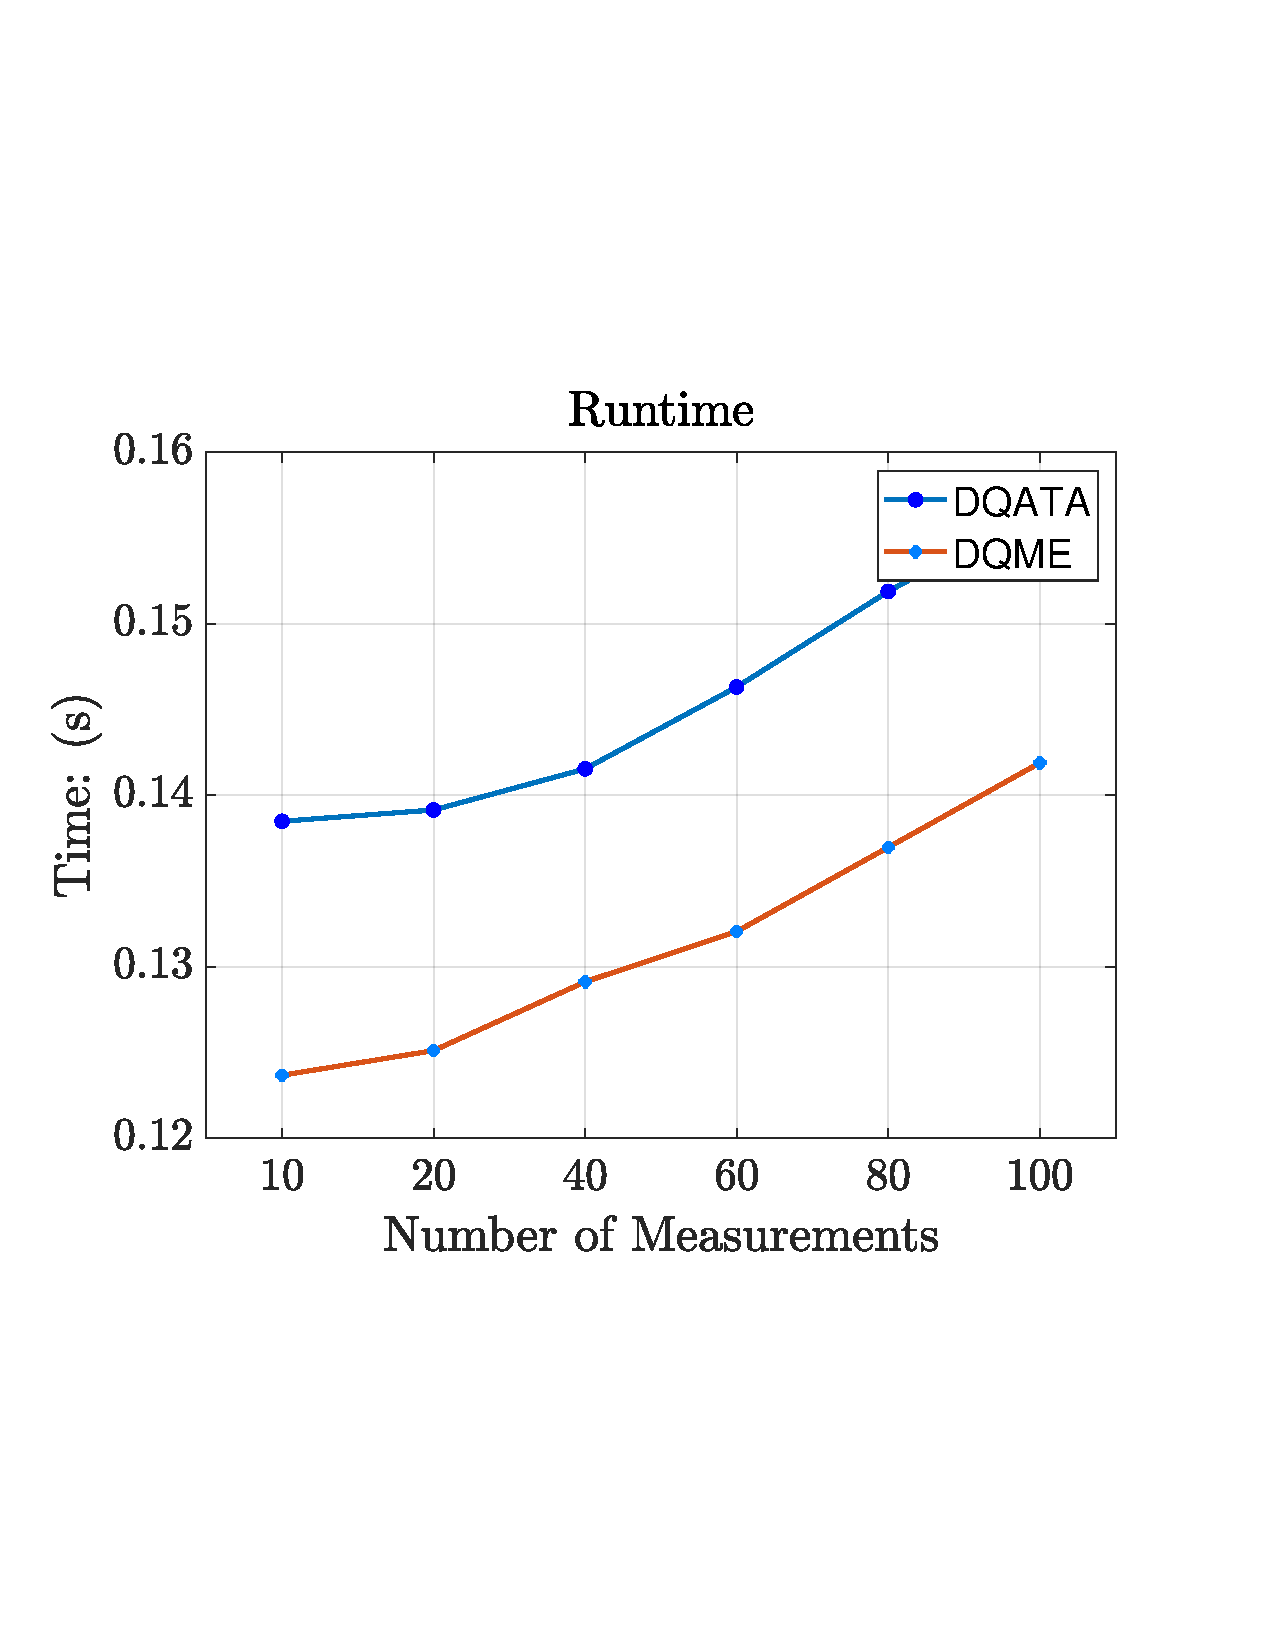
\includegraphics[scale=0.4]{./hand_eye_figures/dq/dq_runtime_cmp}
\caption{Runtime: average time for 100 runs with different numbers of samples.}
\end{figure}

\textbf{Performance under different noisy levels}:
\begin{figure}
\centering
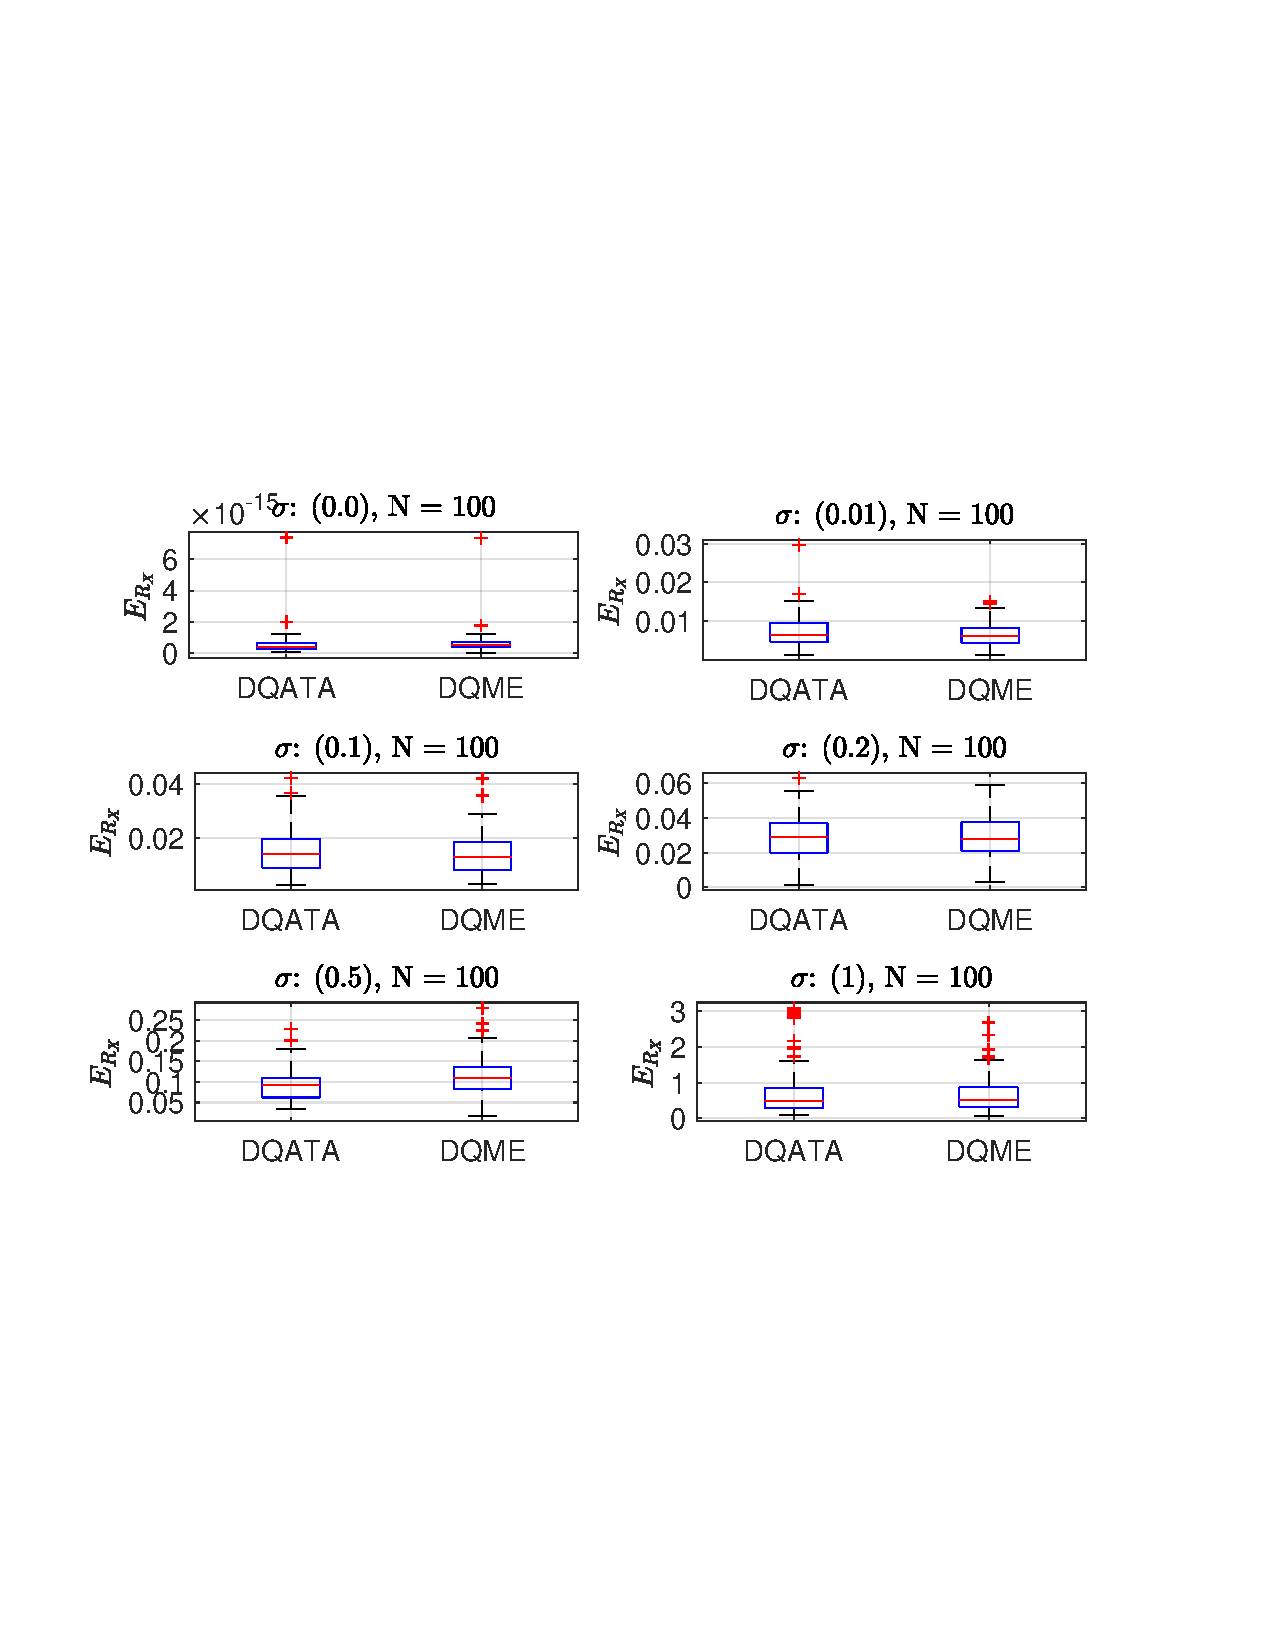
\includegraphics[scale=0.6]{./hand_eye_figures/dq/dq_er_cmp_noise}
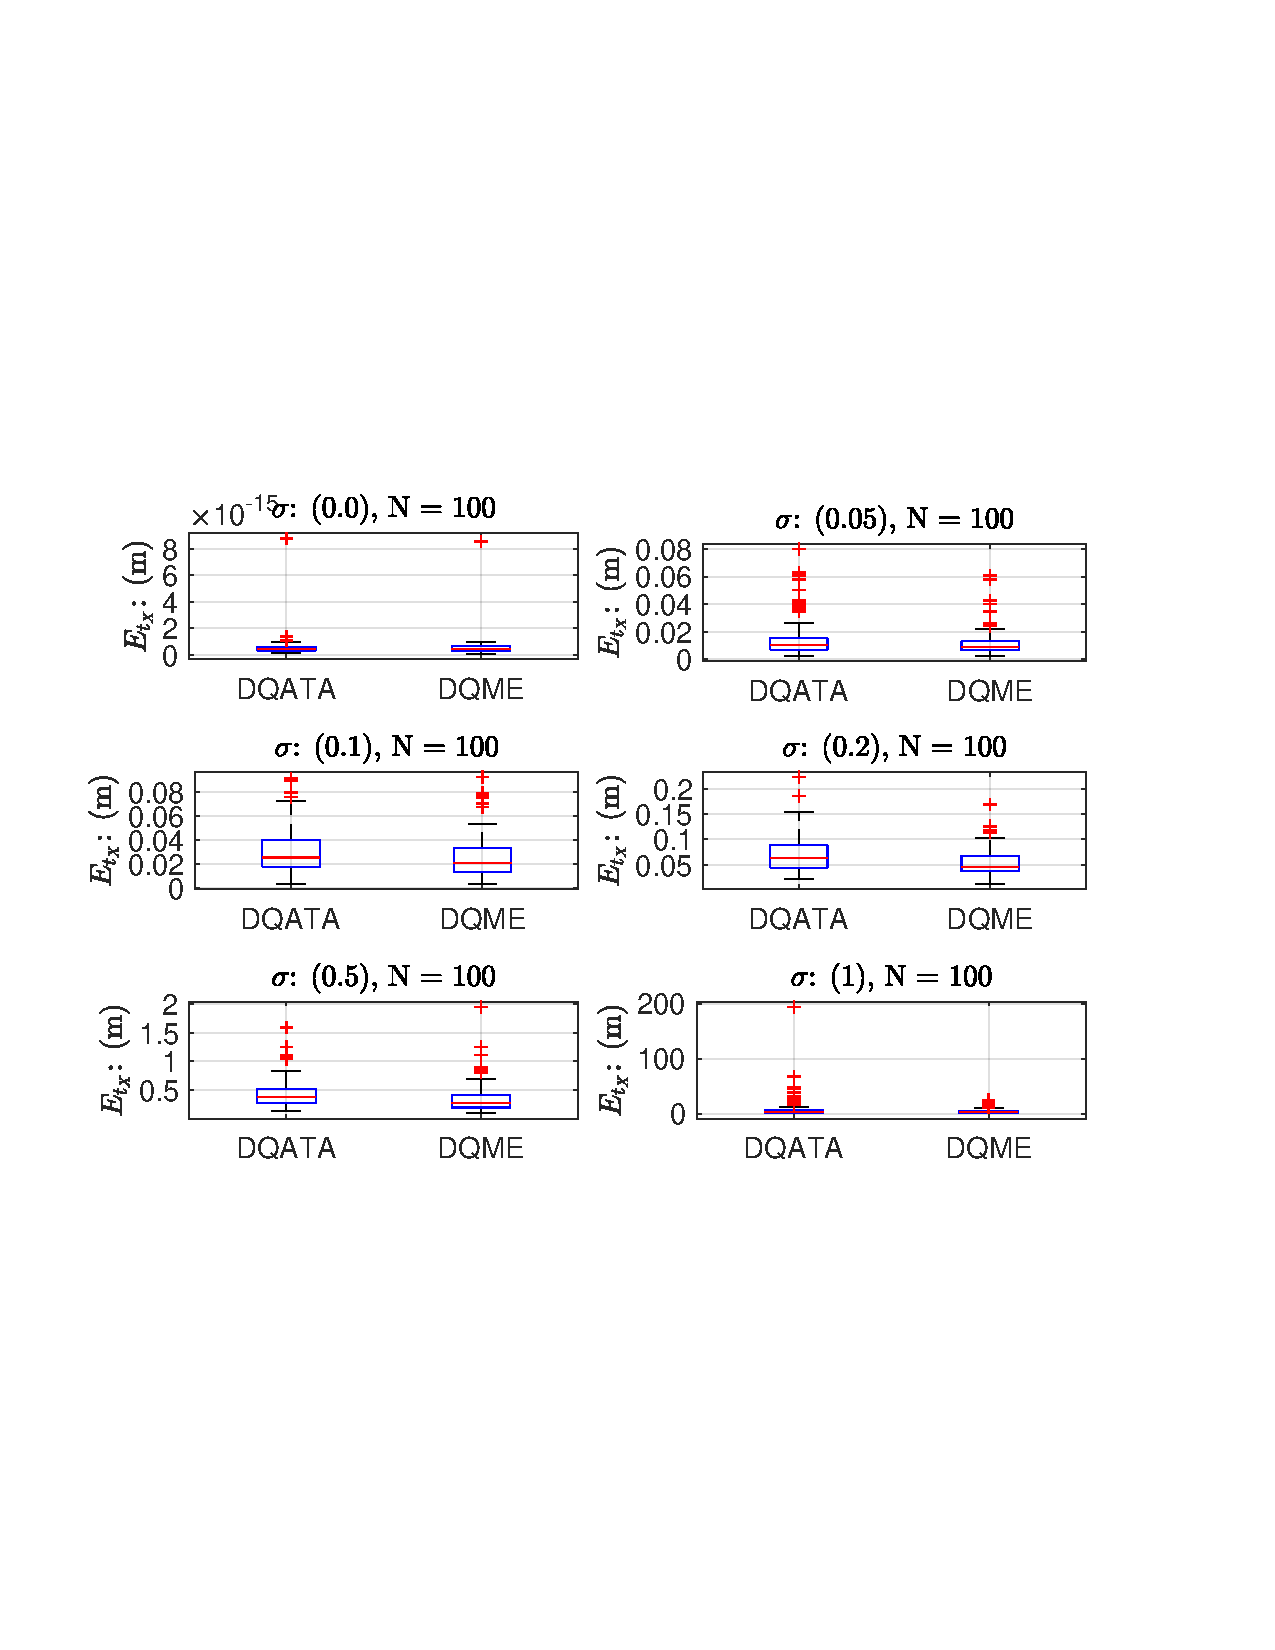
\includegraphics[scale=0.6]{./hand_eye_figures/dq/dq_et_cmp_noise}
\caption{Performance under different noisy levels.}
\end{figure}

\textbf{Performance with different numbers of samples}:
\begin{figure}
\centering
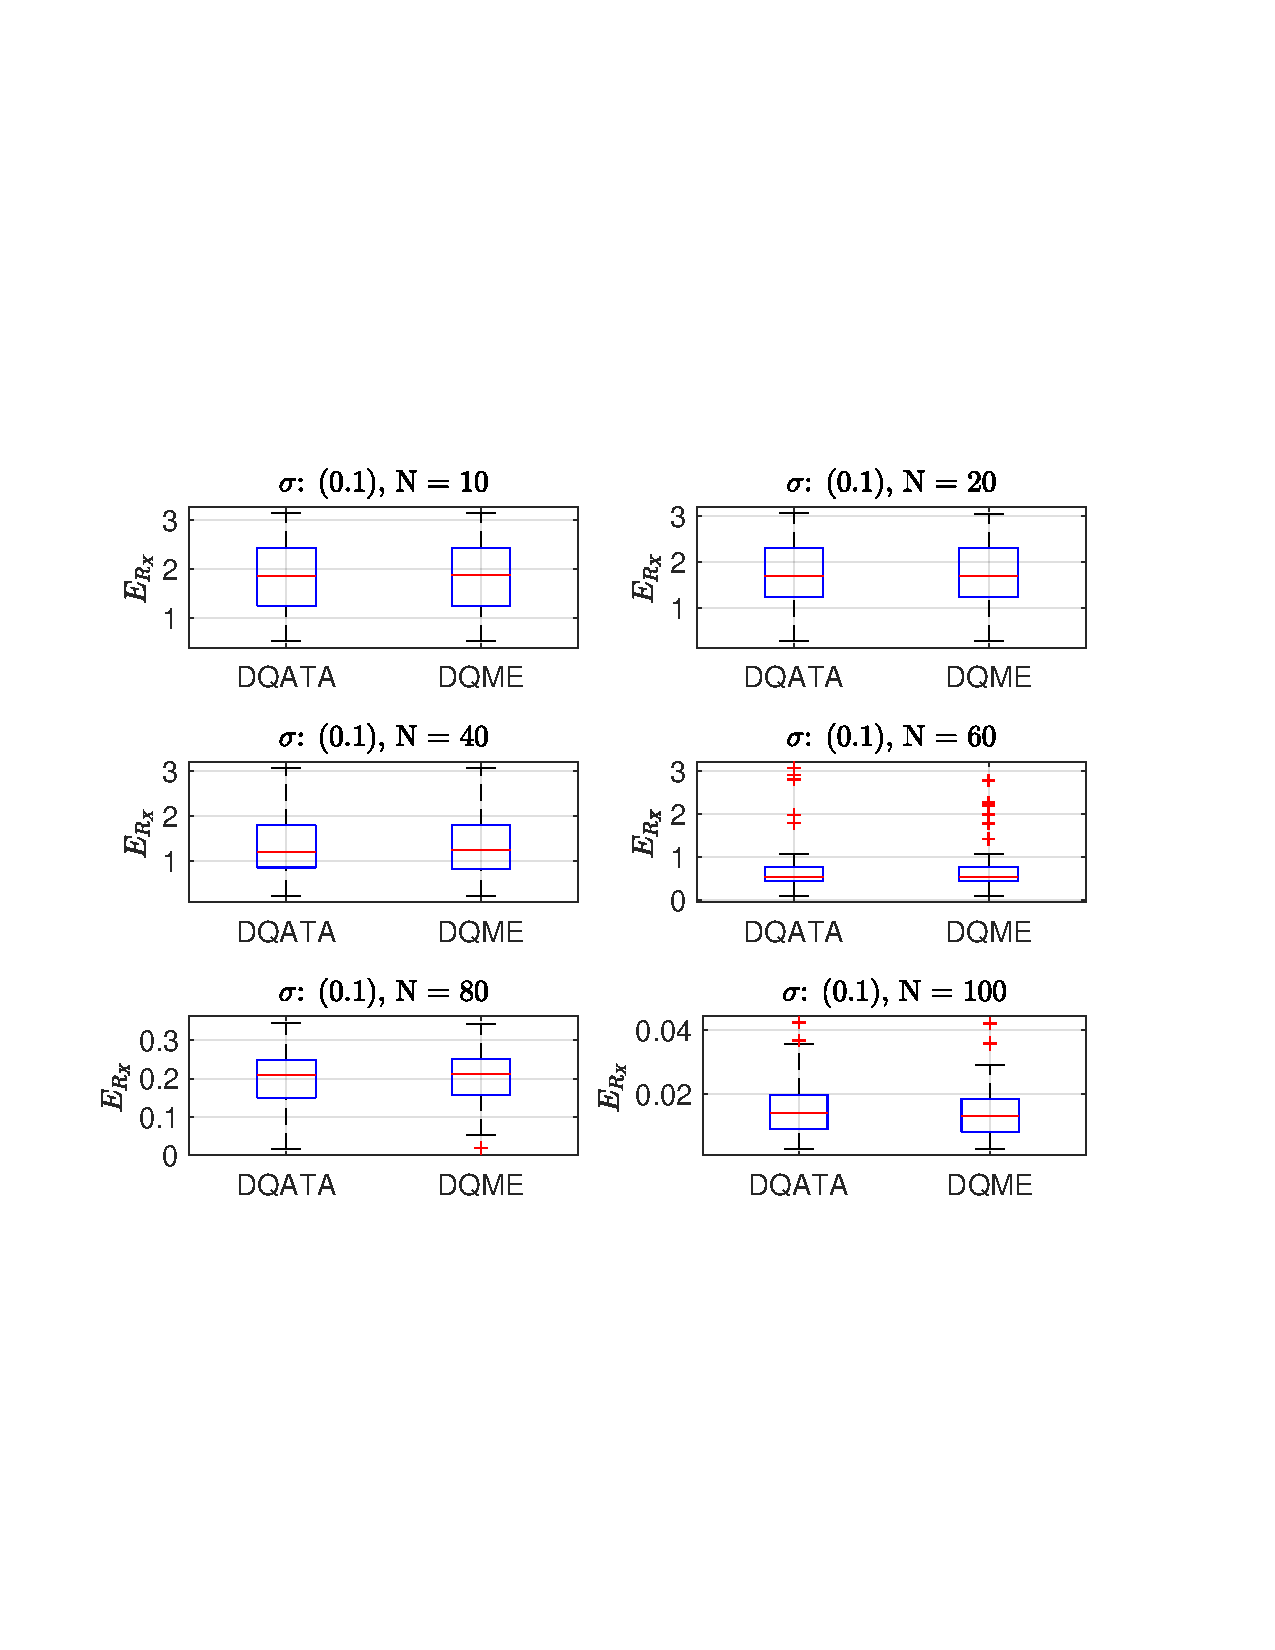
\includegraphics[scale=0.6]{./hand_eye_figures/dq/dq_er_cmp_num}
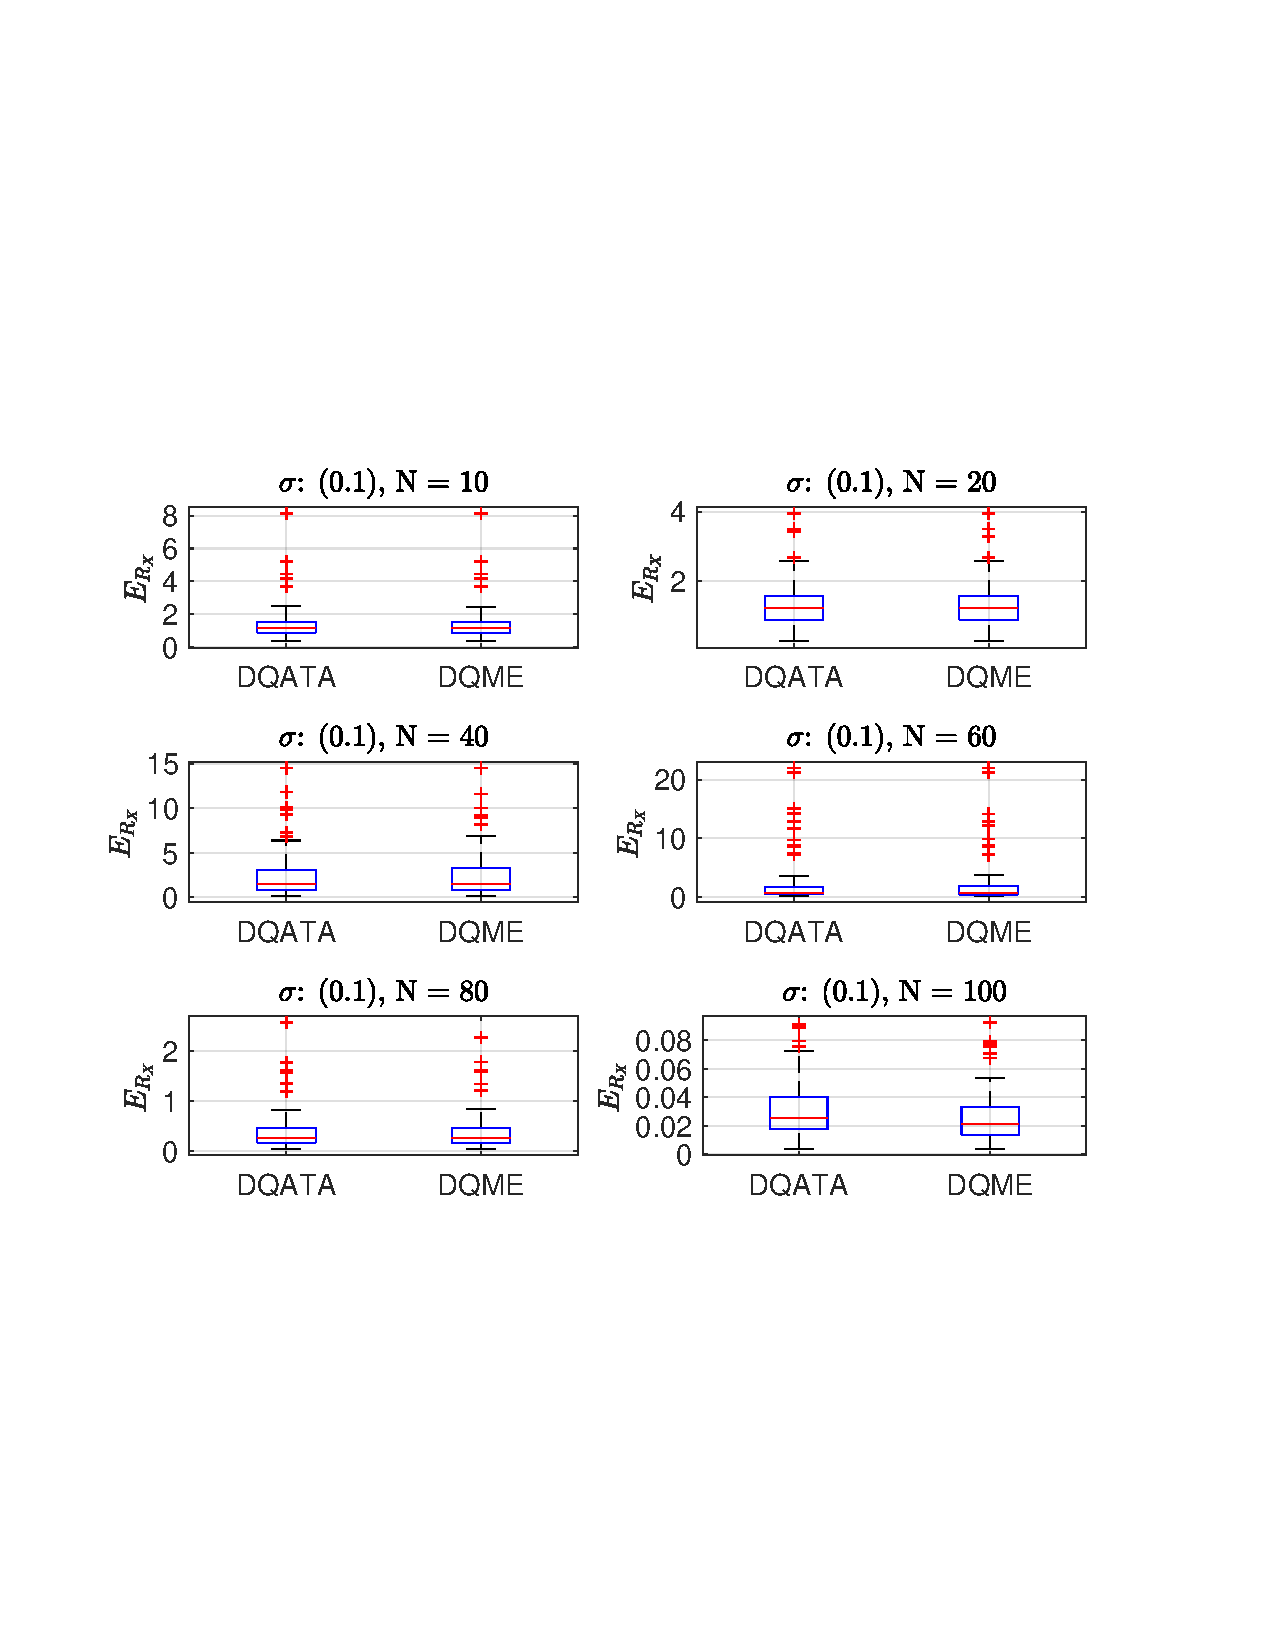
\includegraphics[scale=0.6]{./hand_eye_figures/dq/dq_et_cmp_num}
\caption{Performance under different numbers of samples.}
\end{figure}


\subsection{Comparison on conventional methods}
\begin{itemize}
	\item TSAI~\cite{tsai1989new};
	\item Euclidean Group~\cite{park1994robot};
	\item QSEP~\cite{horaud1995hand};
	\item KRSEP~\cite{andreff1999line};
	\item DQ~\cite{daniilidis1999hand};
	\item IDQ~\cite{malti2010robust};
\end{itemize}

\textbf{Runtime}:
\begin{figure}
\centering
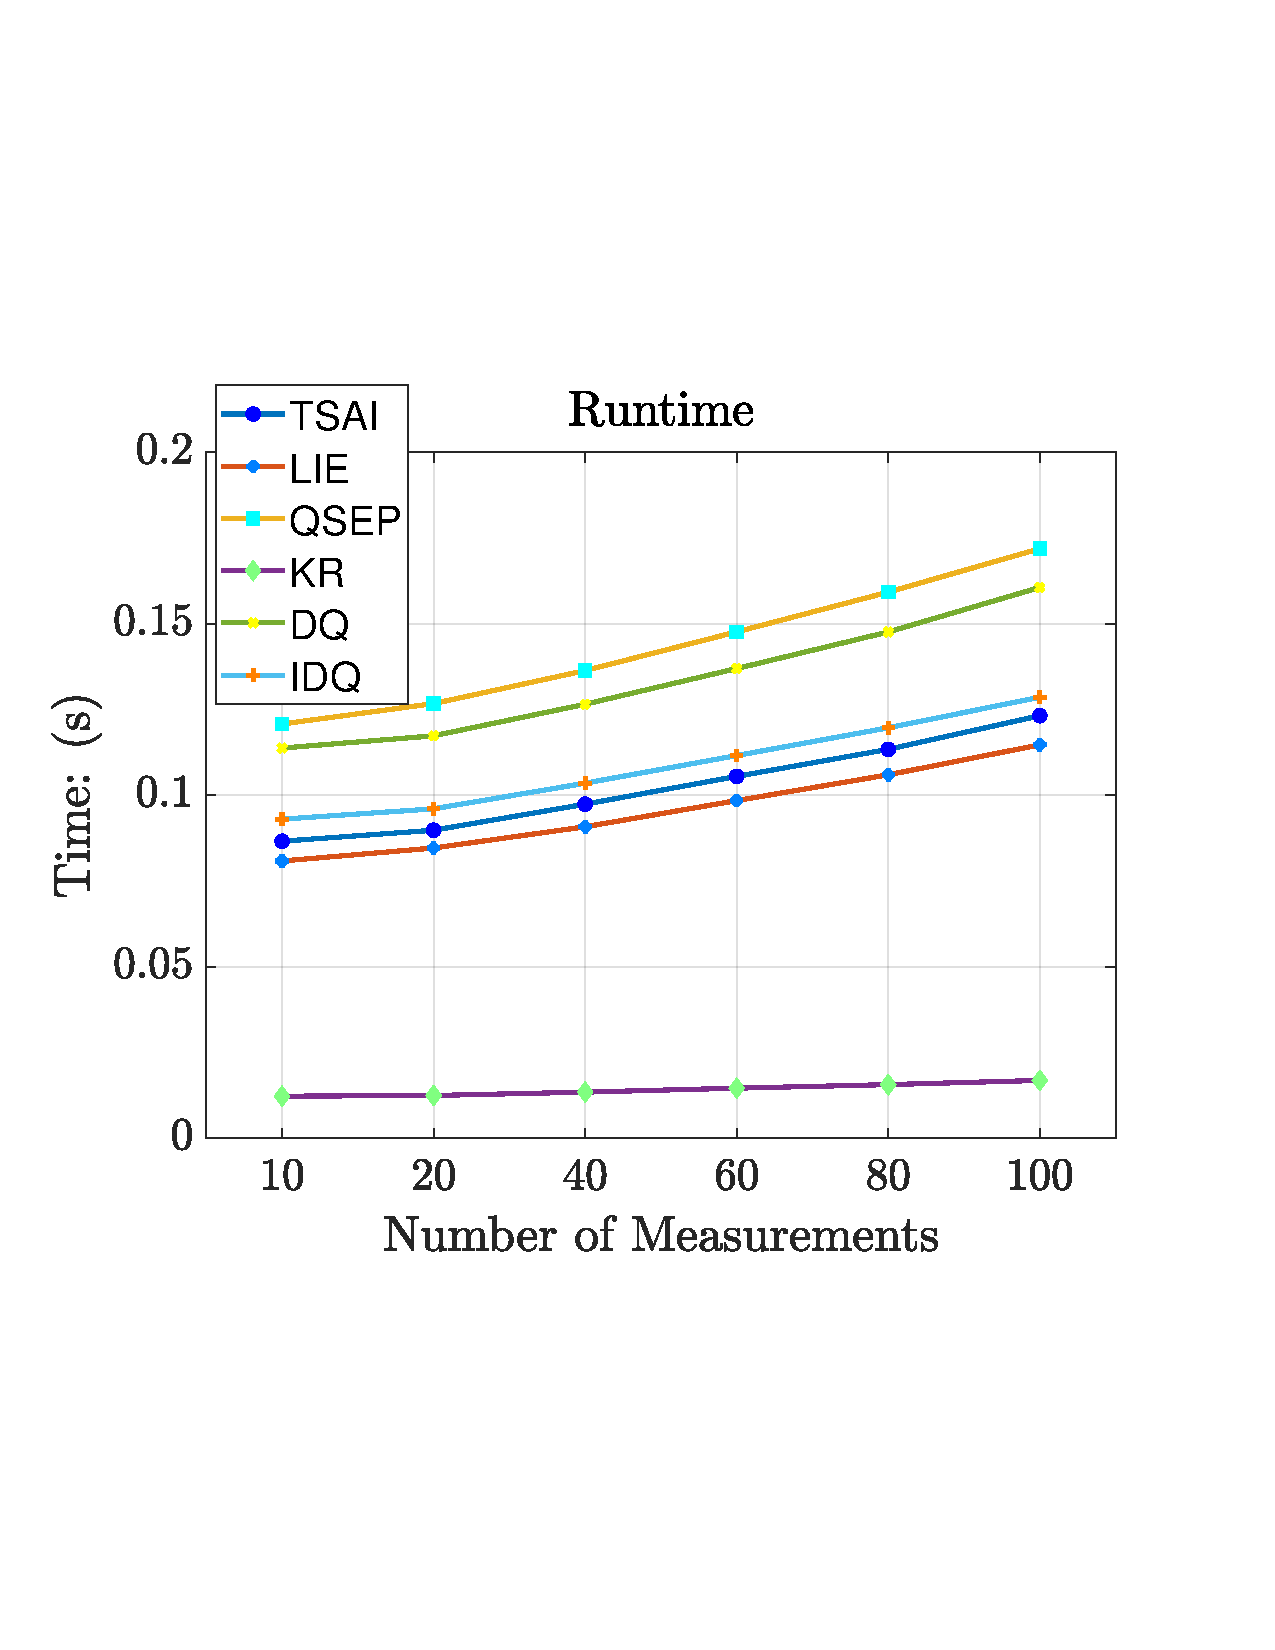
\includegraphics[scale=0.4]{./hand_eye_figures/conv/conv_runtime_cmp}
\caption{Runtime: average time for 100 runs with different numbers of samples.}
\end{figure}

\textbf{Performance under different noisy levels}:
\begin{figure}
\centering
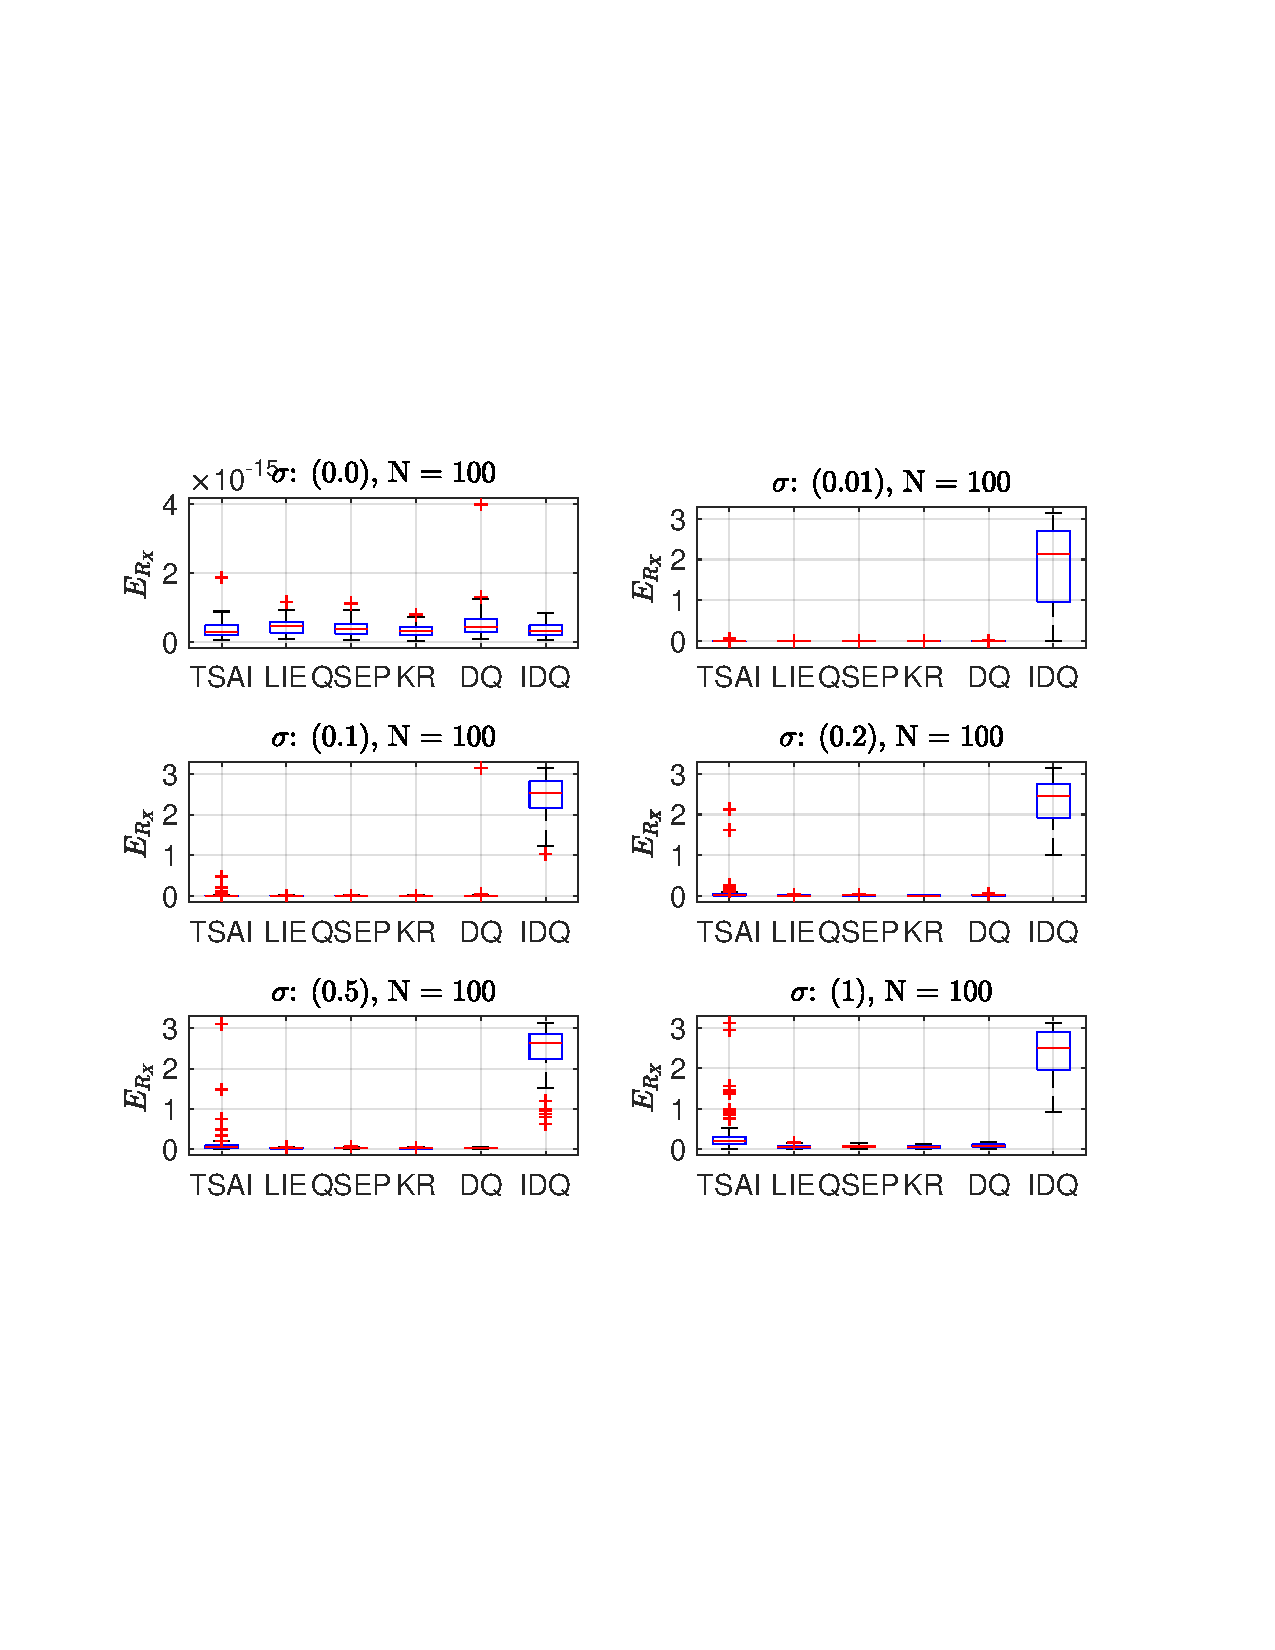
\includegraphics[scale=0.6]{./hand_eye_figures/conv/conv_r_err_cmp}
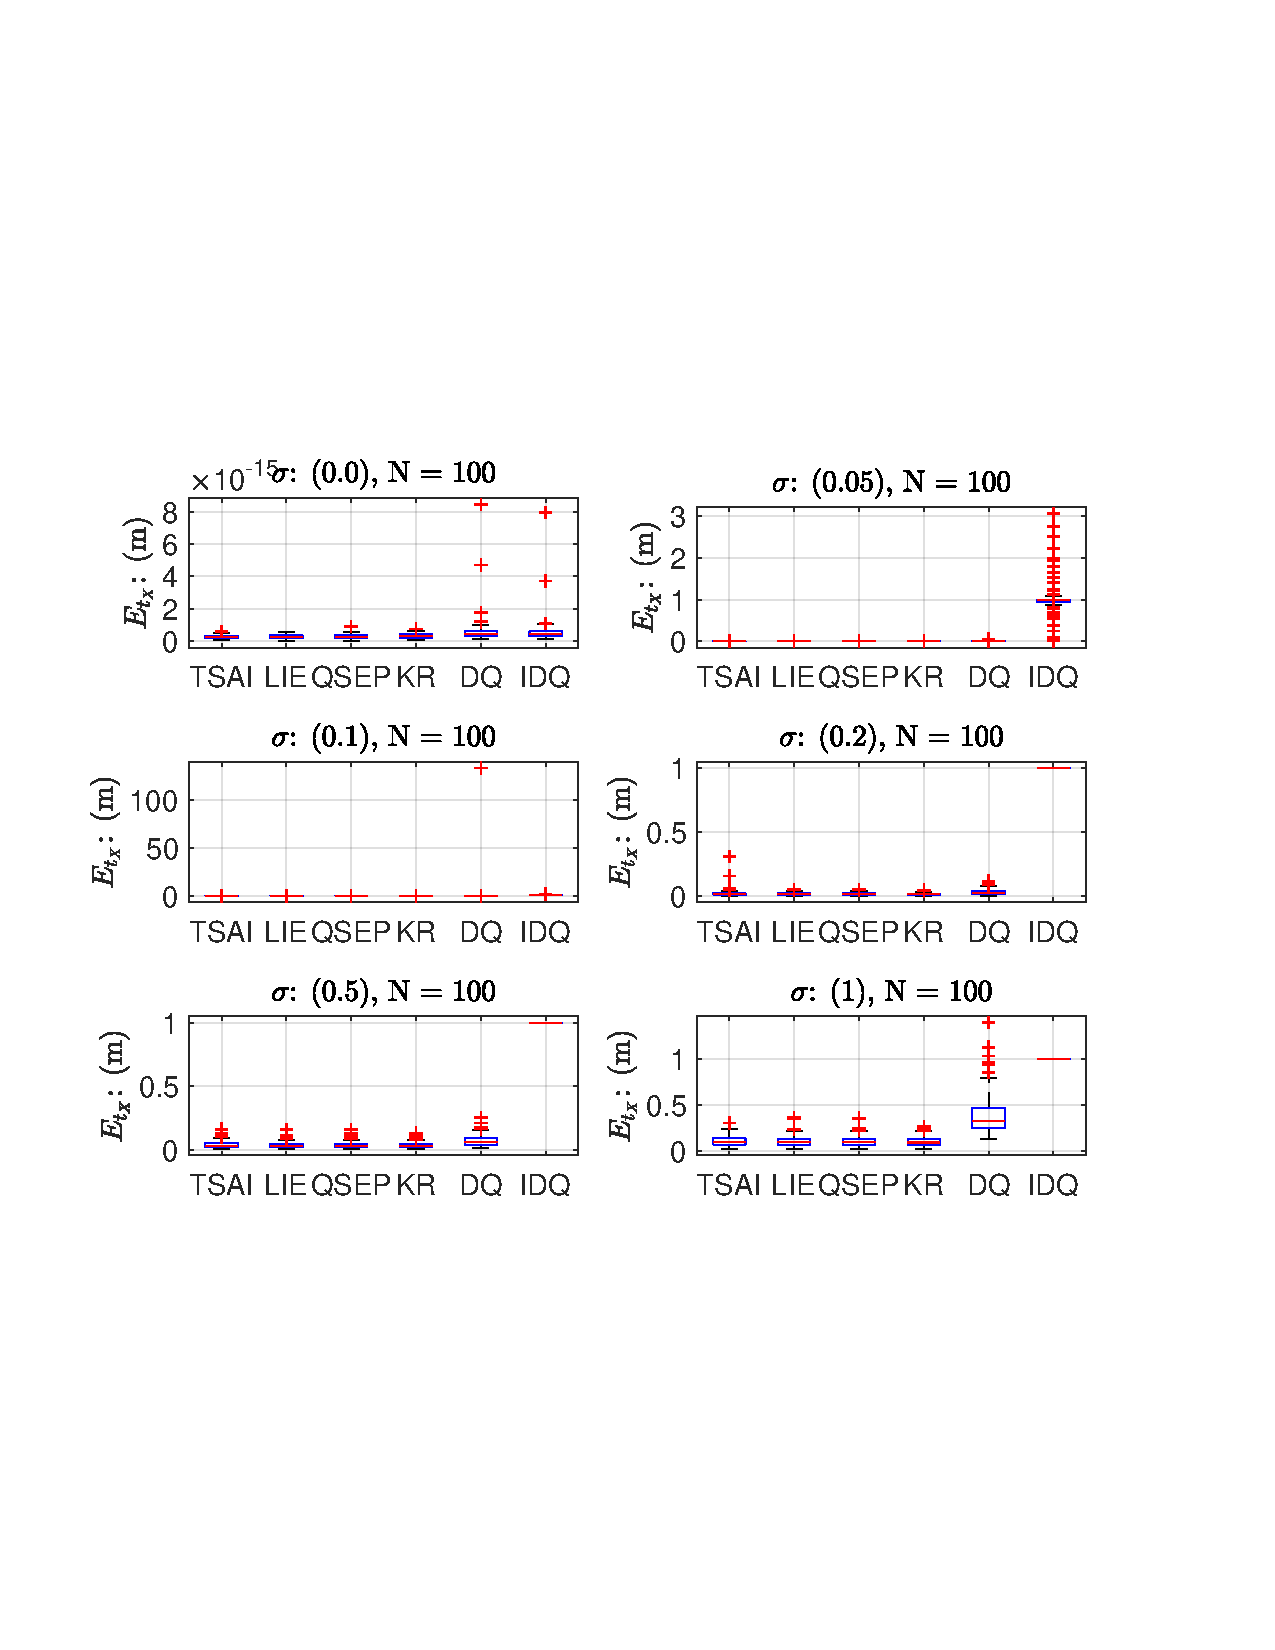
\includegraphics[scale=0.6]{./hand_eye_figures/conv/conv_t_err_cmp}
\caption{Performance under different noisy levels.}
\end{figure}

\textbf{Performance with different numbers of samples}:
\begin{figure}
\centering
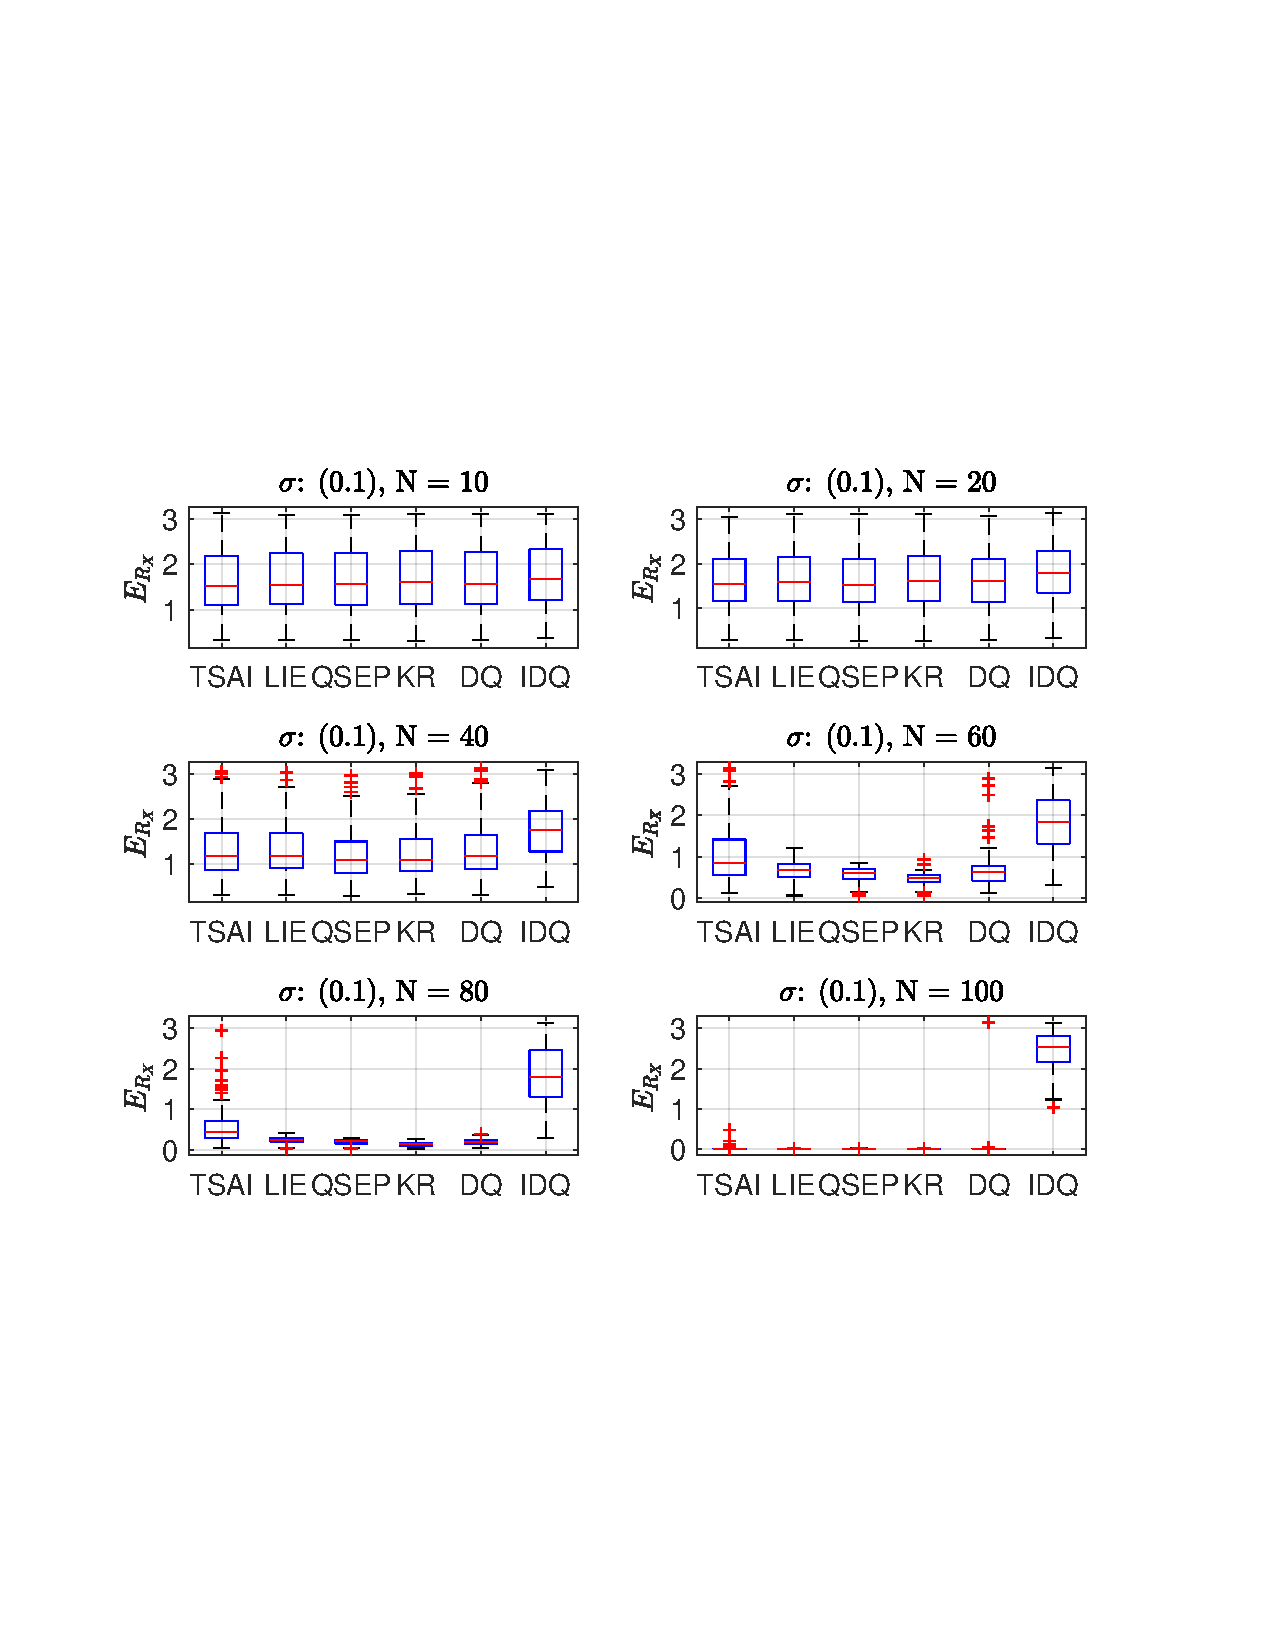
\includegraphics[scale=0.6]{./hand_eye_figures/conv/conv_r_err_cmp1}
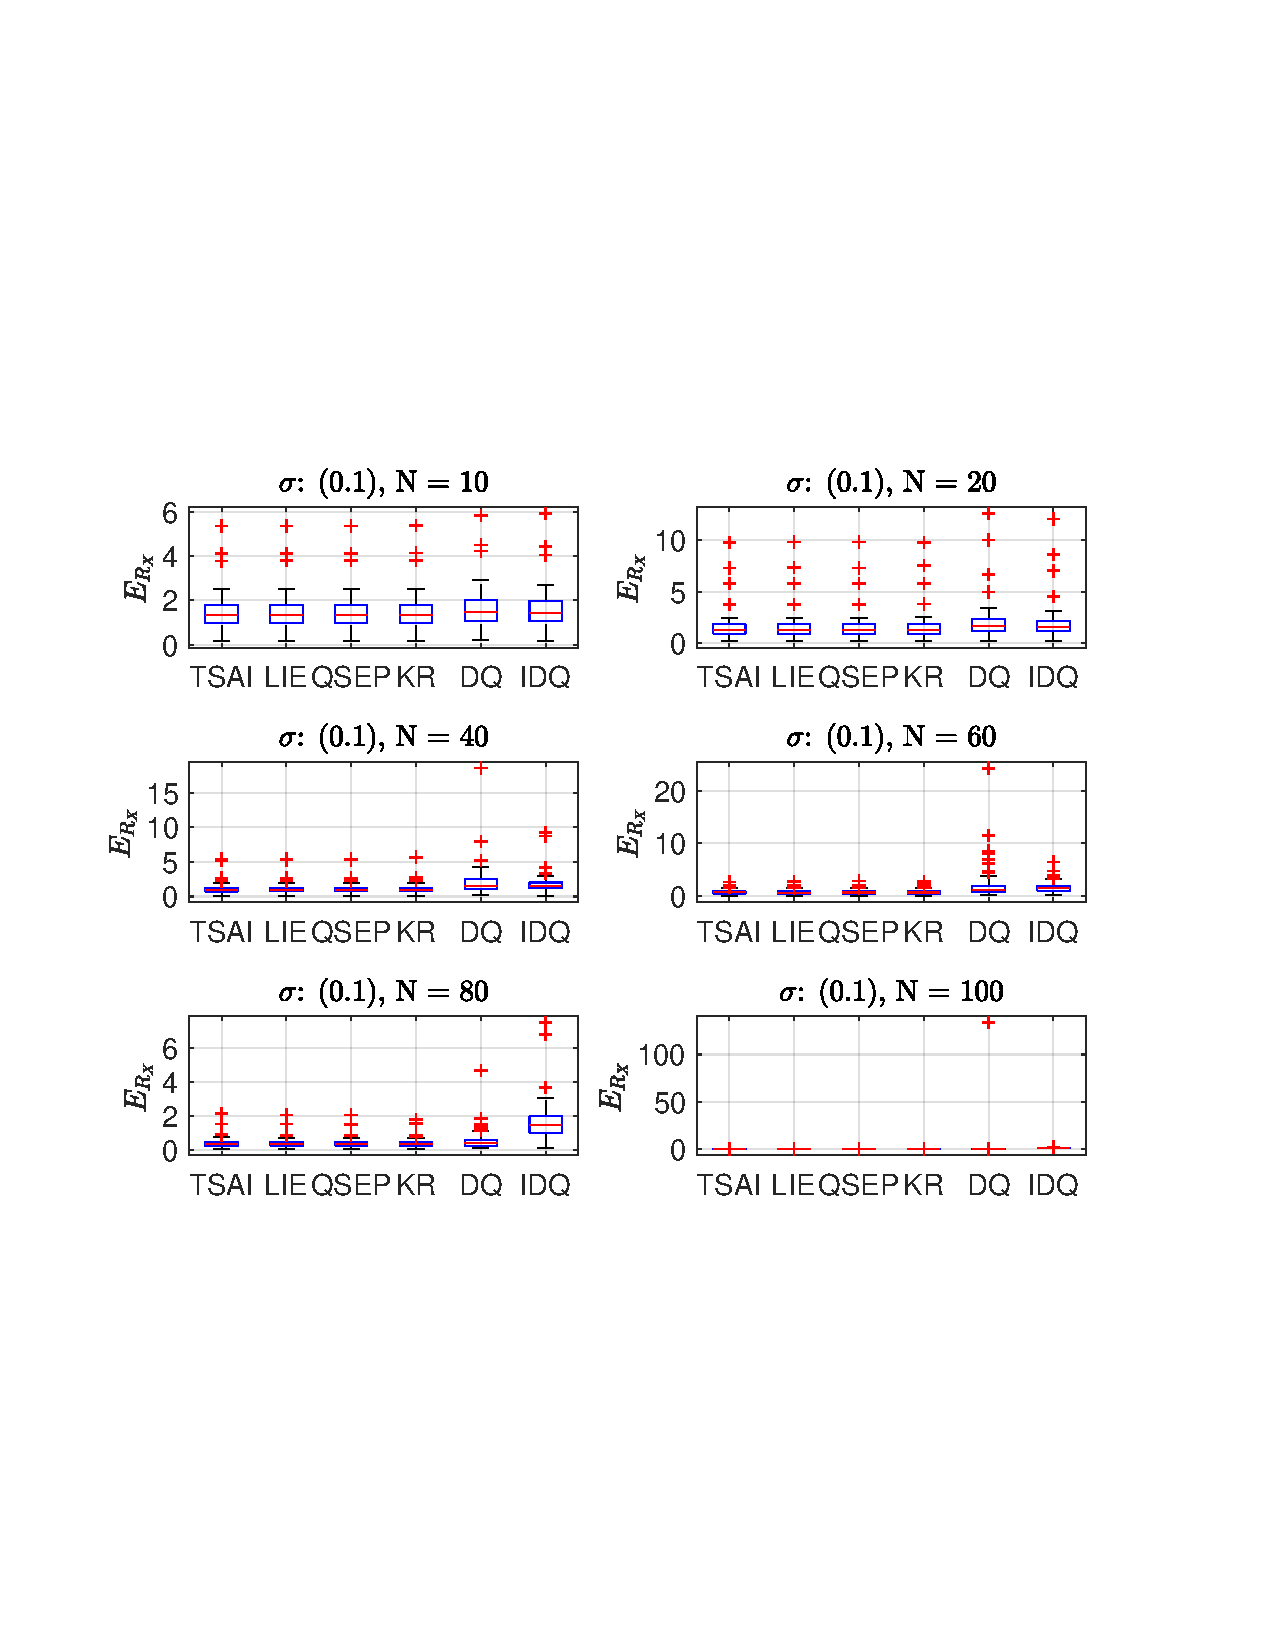
\includegraphics[scale=0.6]{./hand_eye_figures/conv/conv_t_err_cmp1}
\caption{Performance under different numbers of samples.}
\end{figure}

\subsection{SE3 With V.S. Without Initialization}
The following initialization methods are applied:
\begin{itemize}
	\item Kronecker~\cite{andreff1999line};
	\item Euclidean Group~\cite{park1994robot};
	\item Dual Quaternion~\cite{daniilidis1999hand};
\end{itemize}

\textbf{The first test compared the performance under different noisy level}:
\begin{figure}
\centering
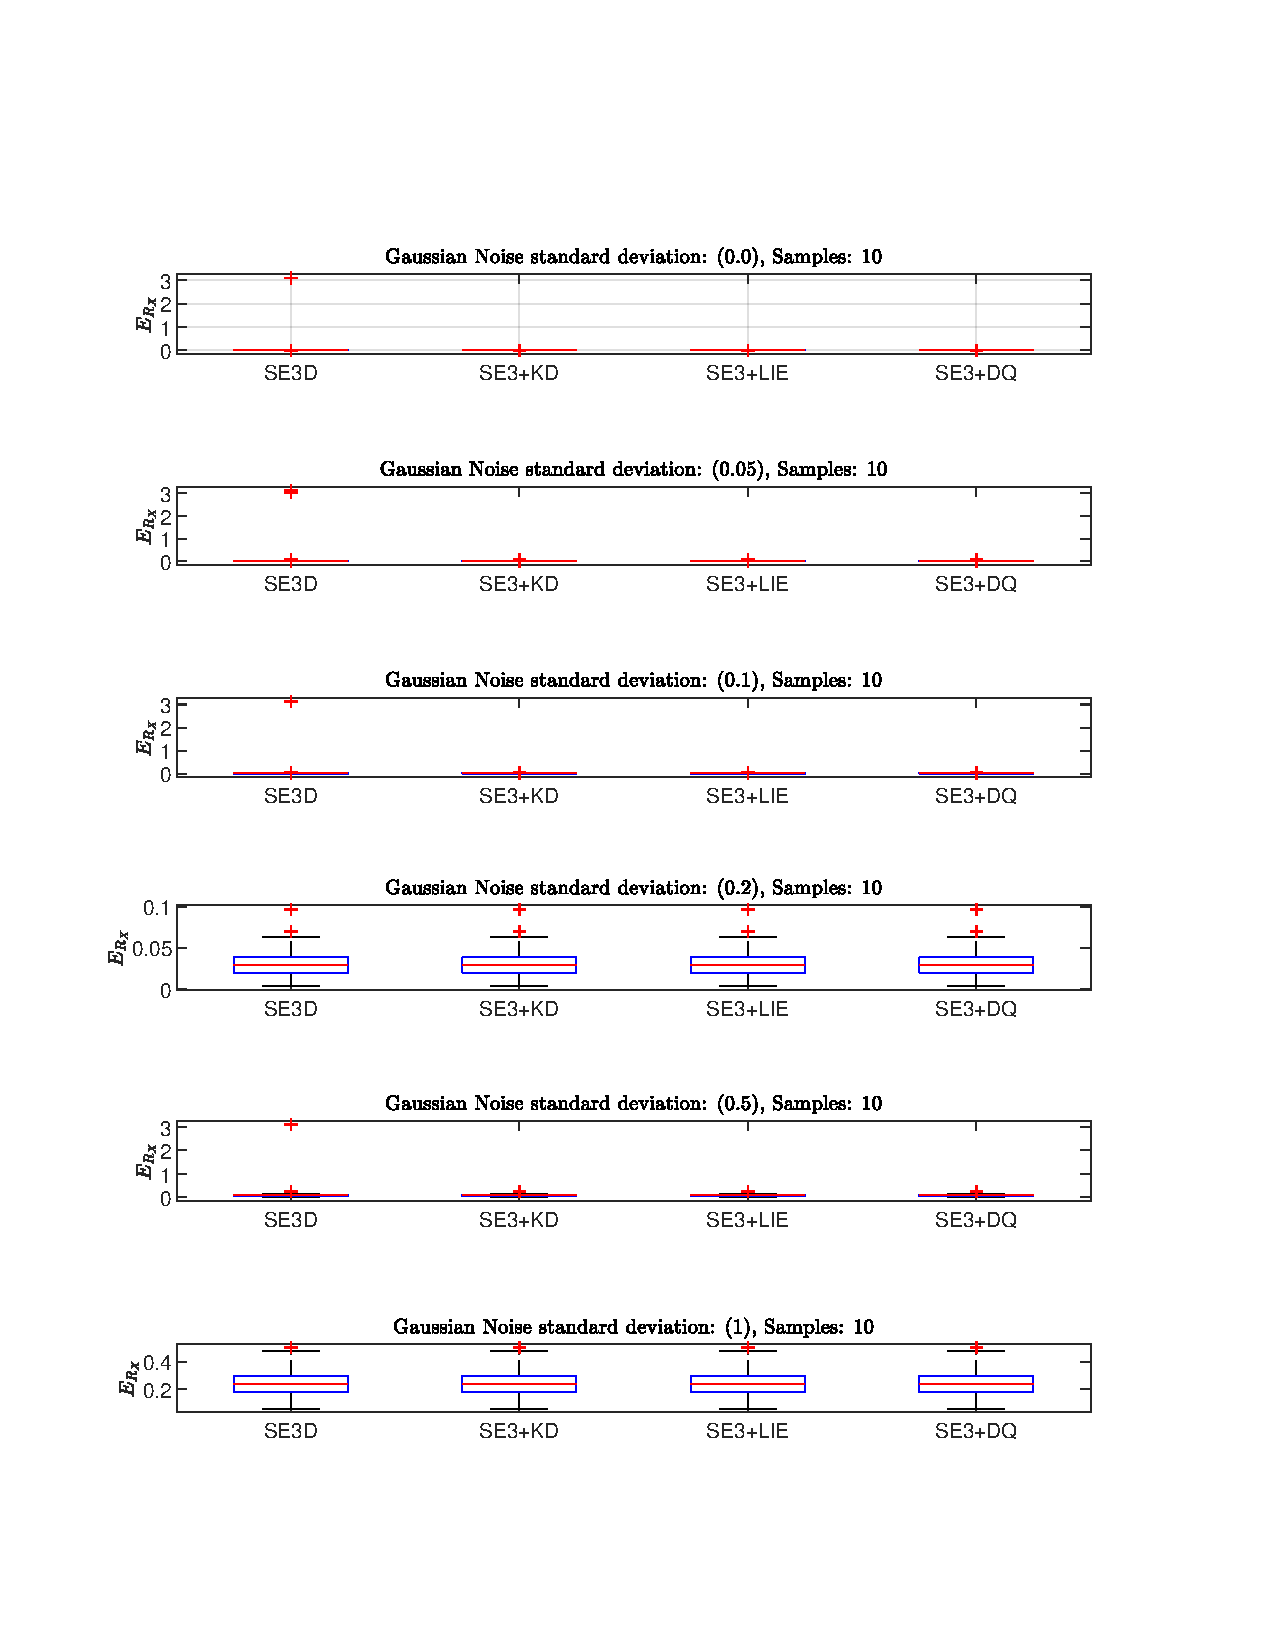
\includegraphics[scale=0.4]{./hand_eye_figures/se3/r_vs_noise}
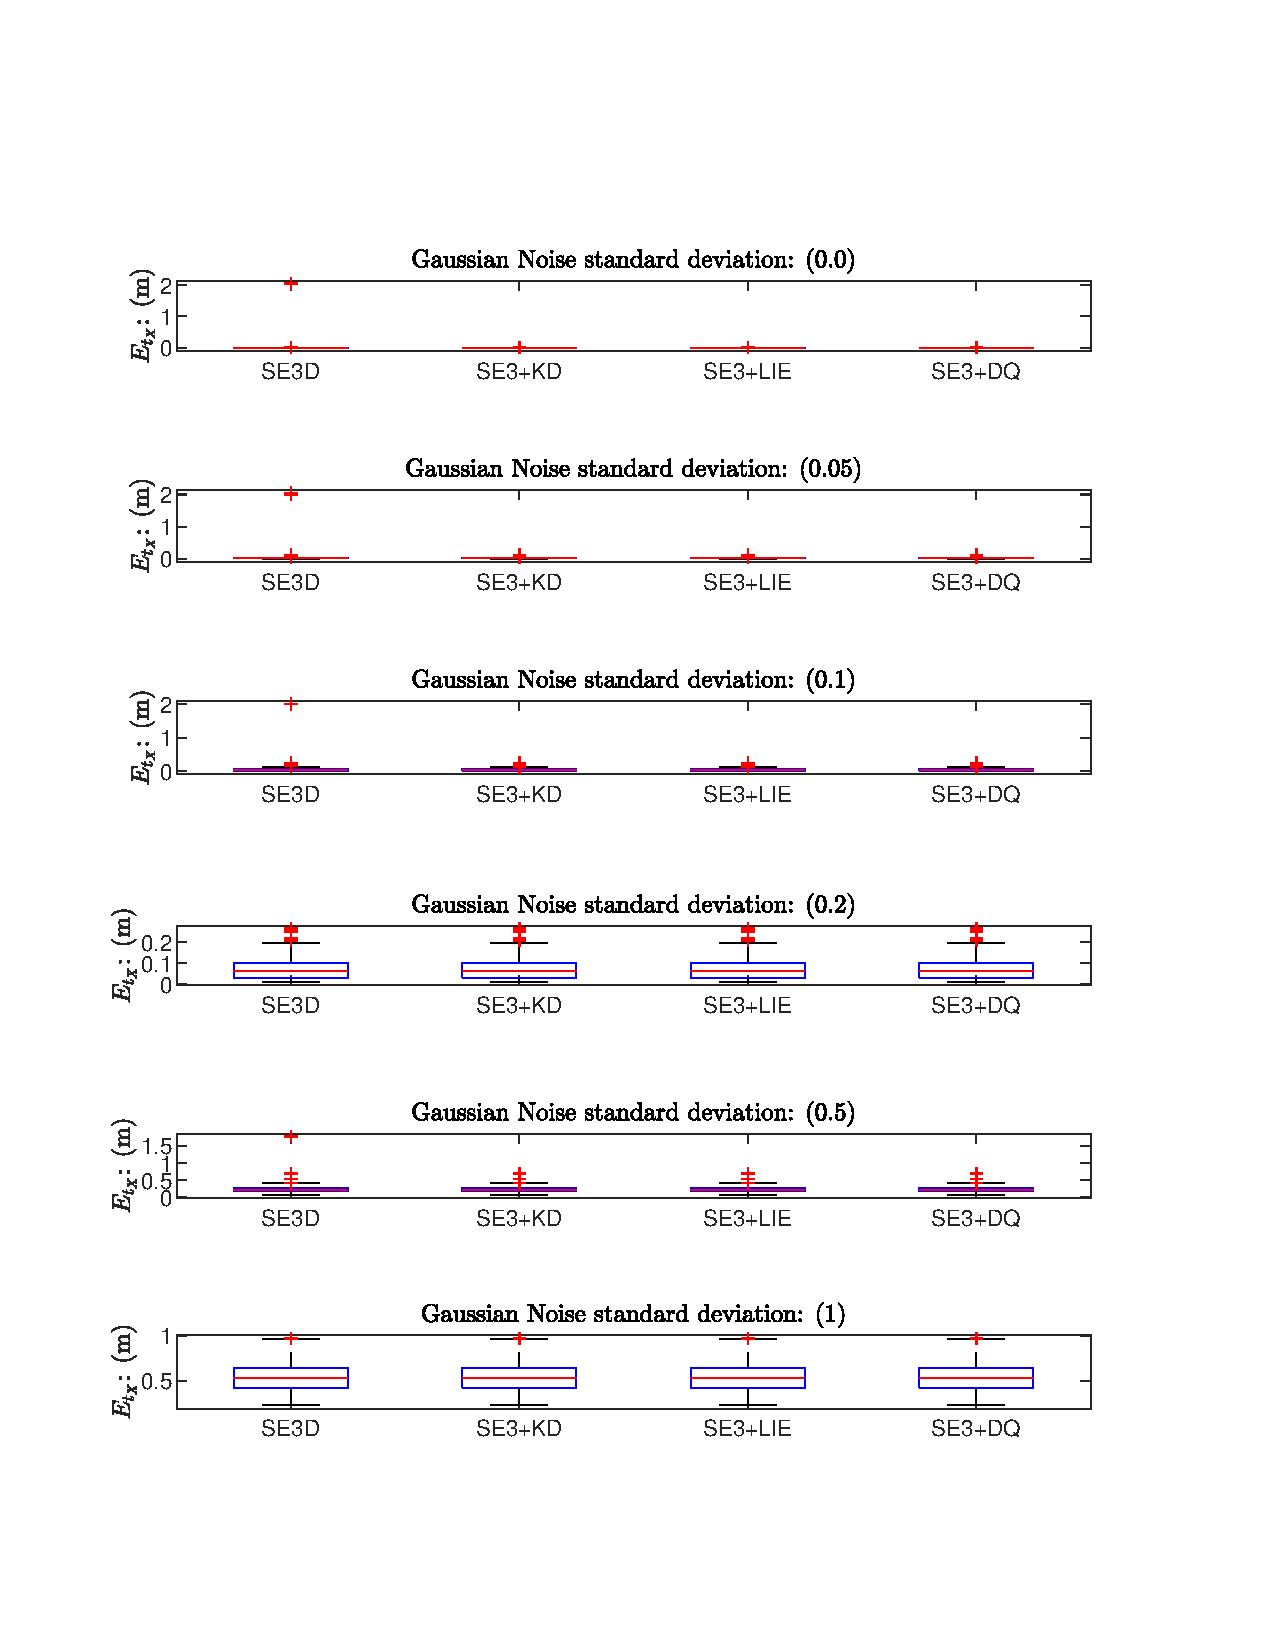
\includegraphics[scale=0.4]{./hand_eye_figures/se3/t_vs_noise}
\caption{Rotation (top) and translational (below) error under $6$ noisy level.}
\end{figure}
The initialization will slightly improve the accuracy: at least less outliers. With regarding to the final accuracy, it will not change to much.

\textbf{The first test compared the performance under different number of samples}:
\begin{figure}
\centering
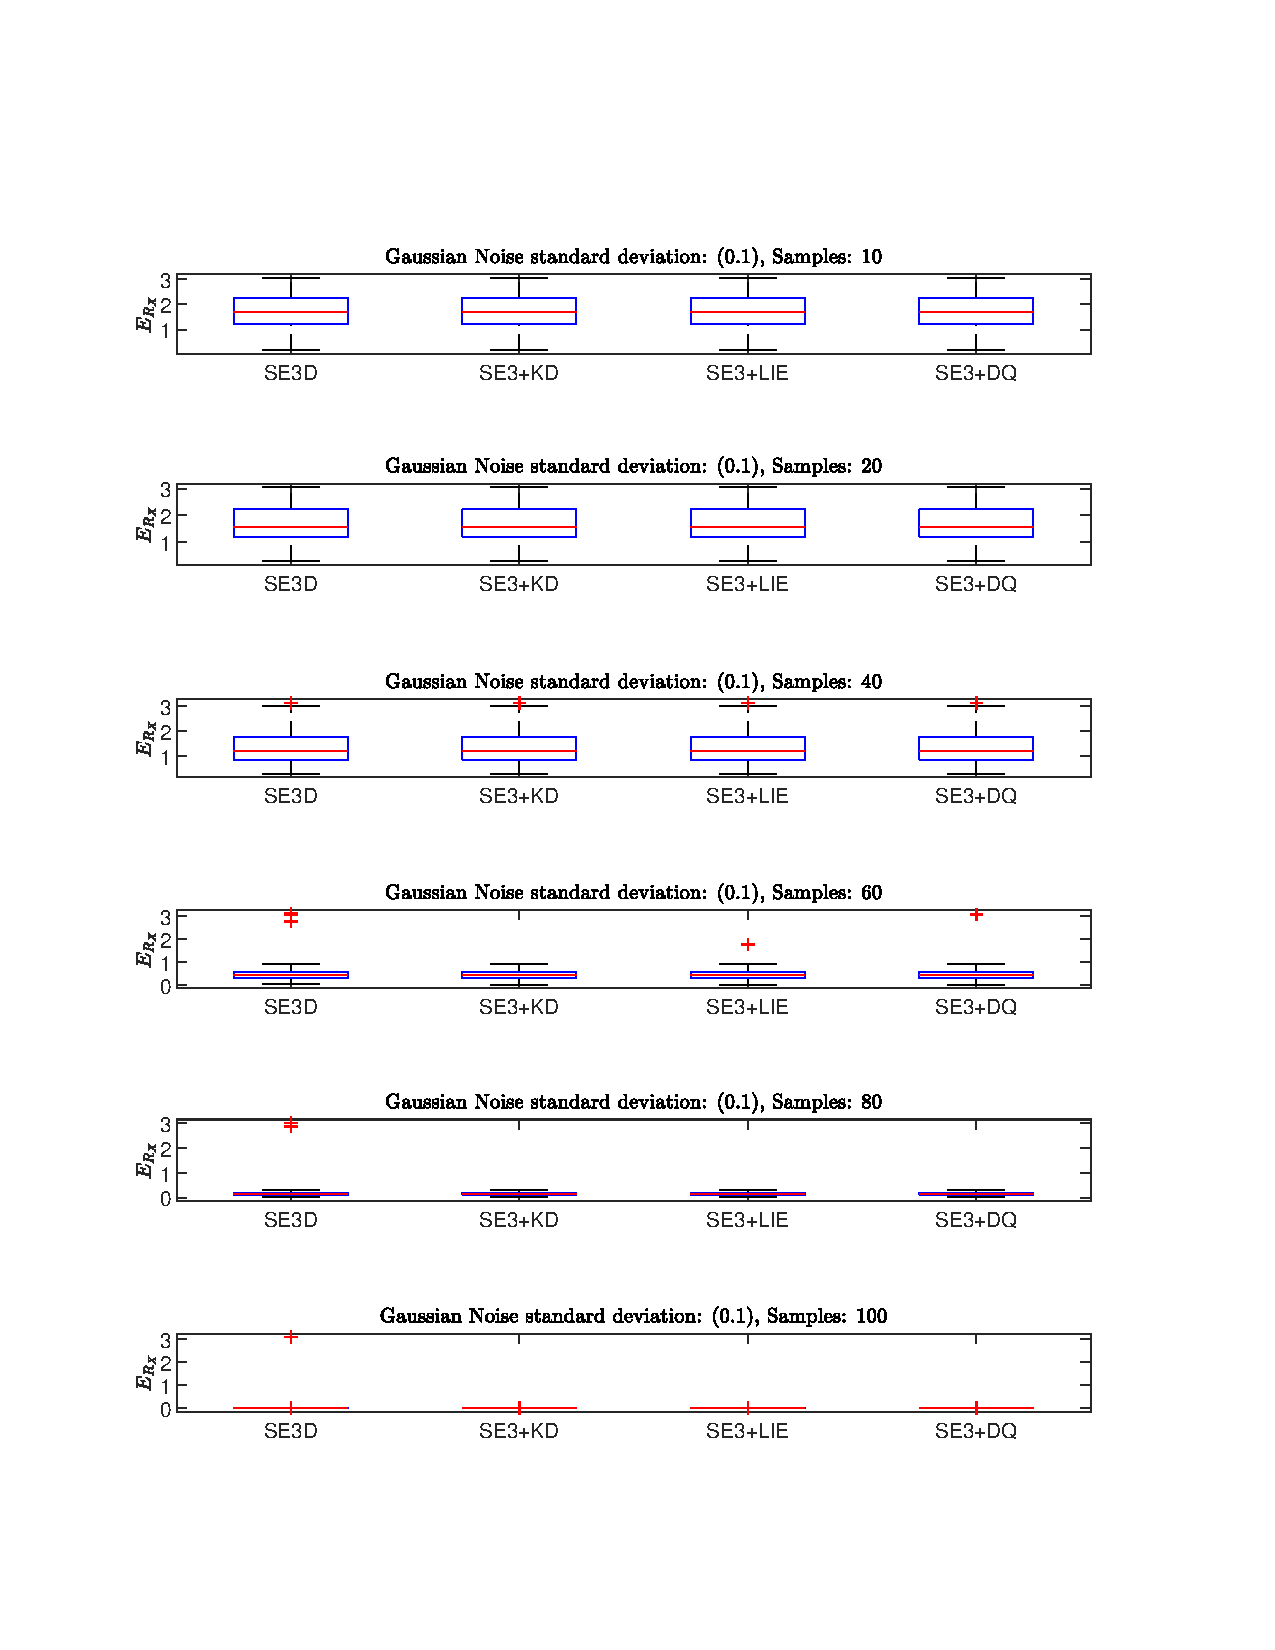
\includegraphics[scale=0.4]{./hand_eye_figures/se3/r_vs_num}
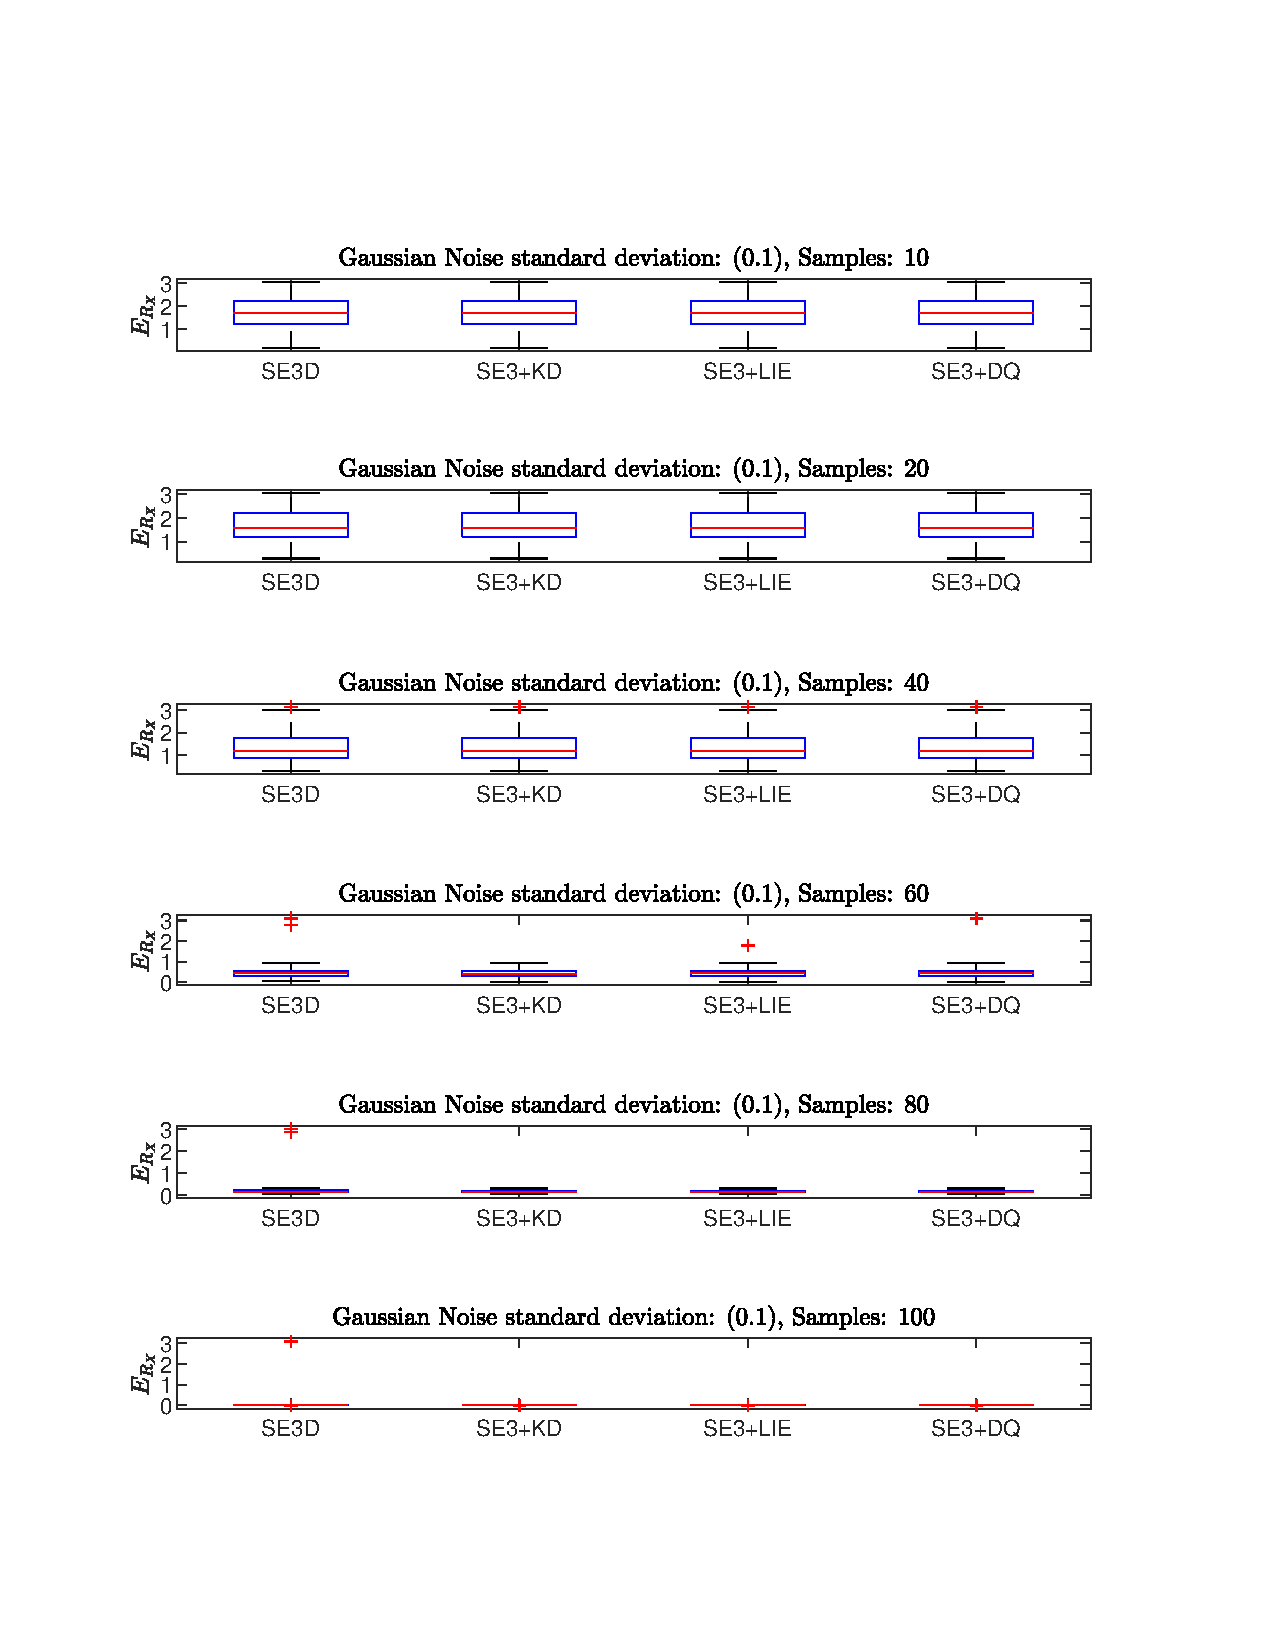
\includegraphics[scale=0.4]{./hand_eye_figures/se3/t_vs_num}
\caption{Rotation (top) and translational (below) error under $6$ noisy level.}
\end{figure}
It is clear that more samples will significantly improve the accuracy.

\textbf{With regarding to the speed, no significant changes have been monitored. So anyone can be used as the initialization method.}


\section{Real Data Experiment}
In this section, experiments are carried out on real data. Two real dataset publicly available are used:
\begin{itemize}
\item Data captured with Xtion RGB-D sensors provided by
the authors of~\cite{brookshire2013extrinsic}. For details about data collection, the extraction of relative
pose measurements, and ground truth, see~\cite{brookshire2013extrinsic}.
\item Datasets "\textbf{Primesense{\textunderscore}1}", "\textbf{Primesense{\textunderscore}2}", "\textbf{robot{\textunderscore}arm{\textunderscore}w{\textunderscore}color{\textunderscore}camera{\textunderscore}real}", "\textbf{robot{\textunderscore}arm{\textunderscore}w{\textunderscore}color{\textunderscore}camera{\textunderscore}sim}" provided by
the authors of~\cite{furrer2018evaluation}. However, no ground truth can be obtained. As a result, we will evaluate the RMSE values.
\end{itemize}

\begin{figure}
\centering
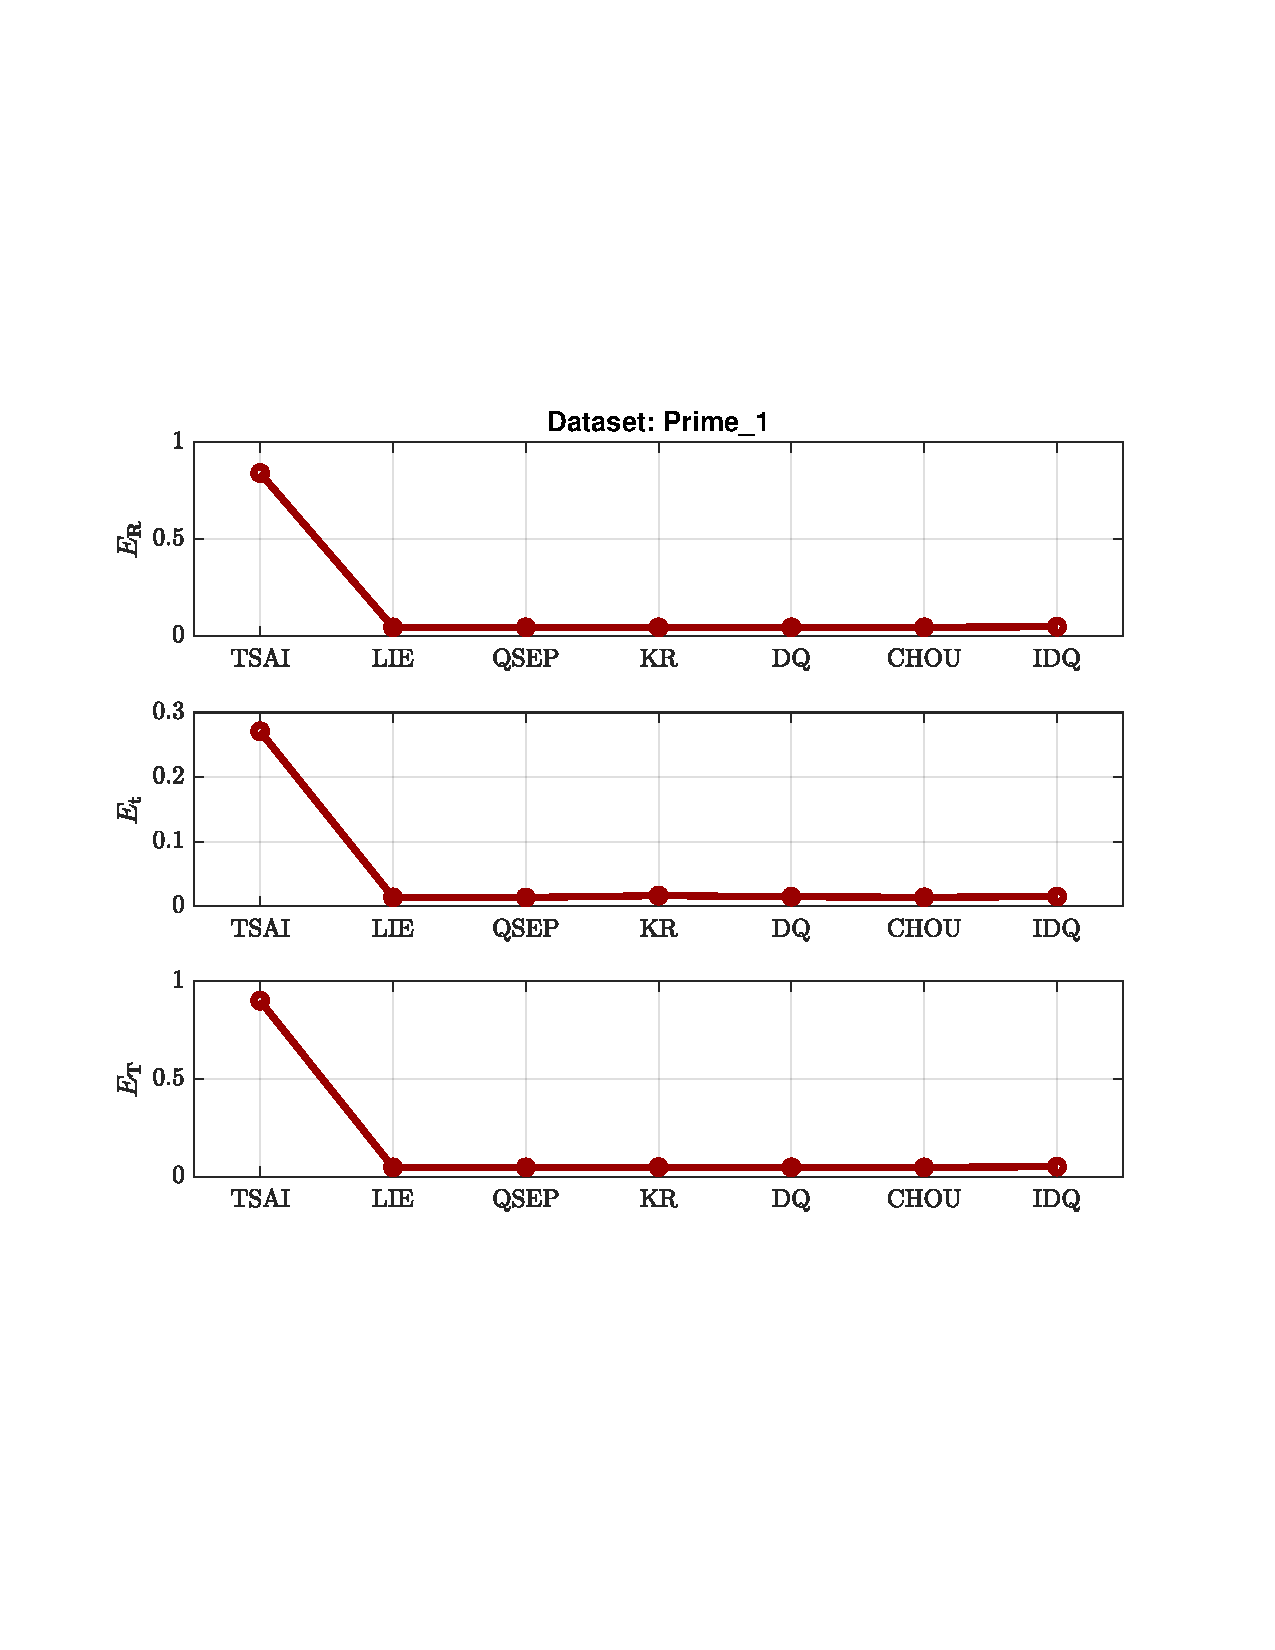
\includegraphics[scale=0.7]{./hand_eye_figures/real/Result_Prime_1}
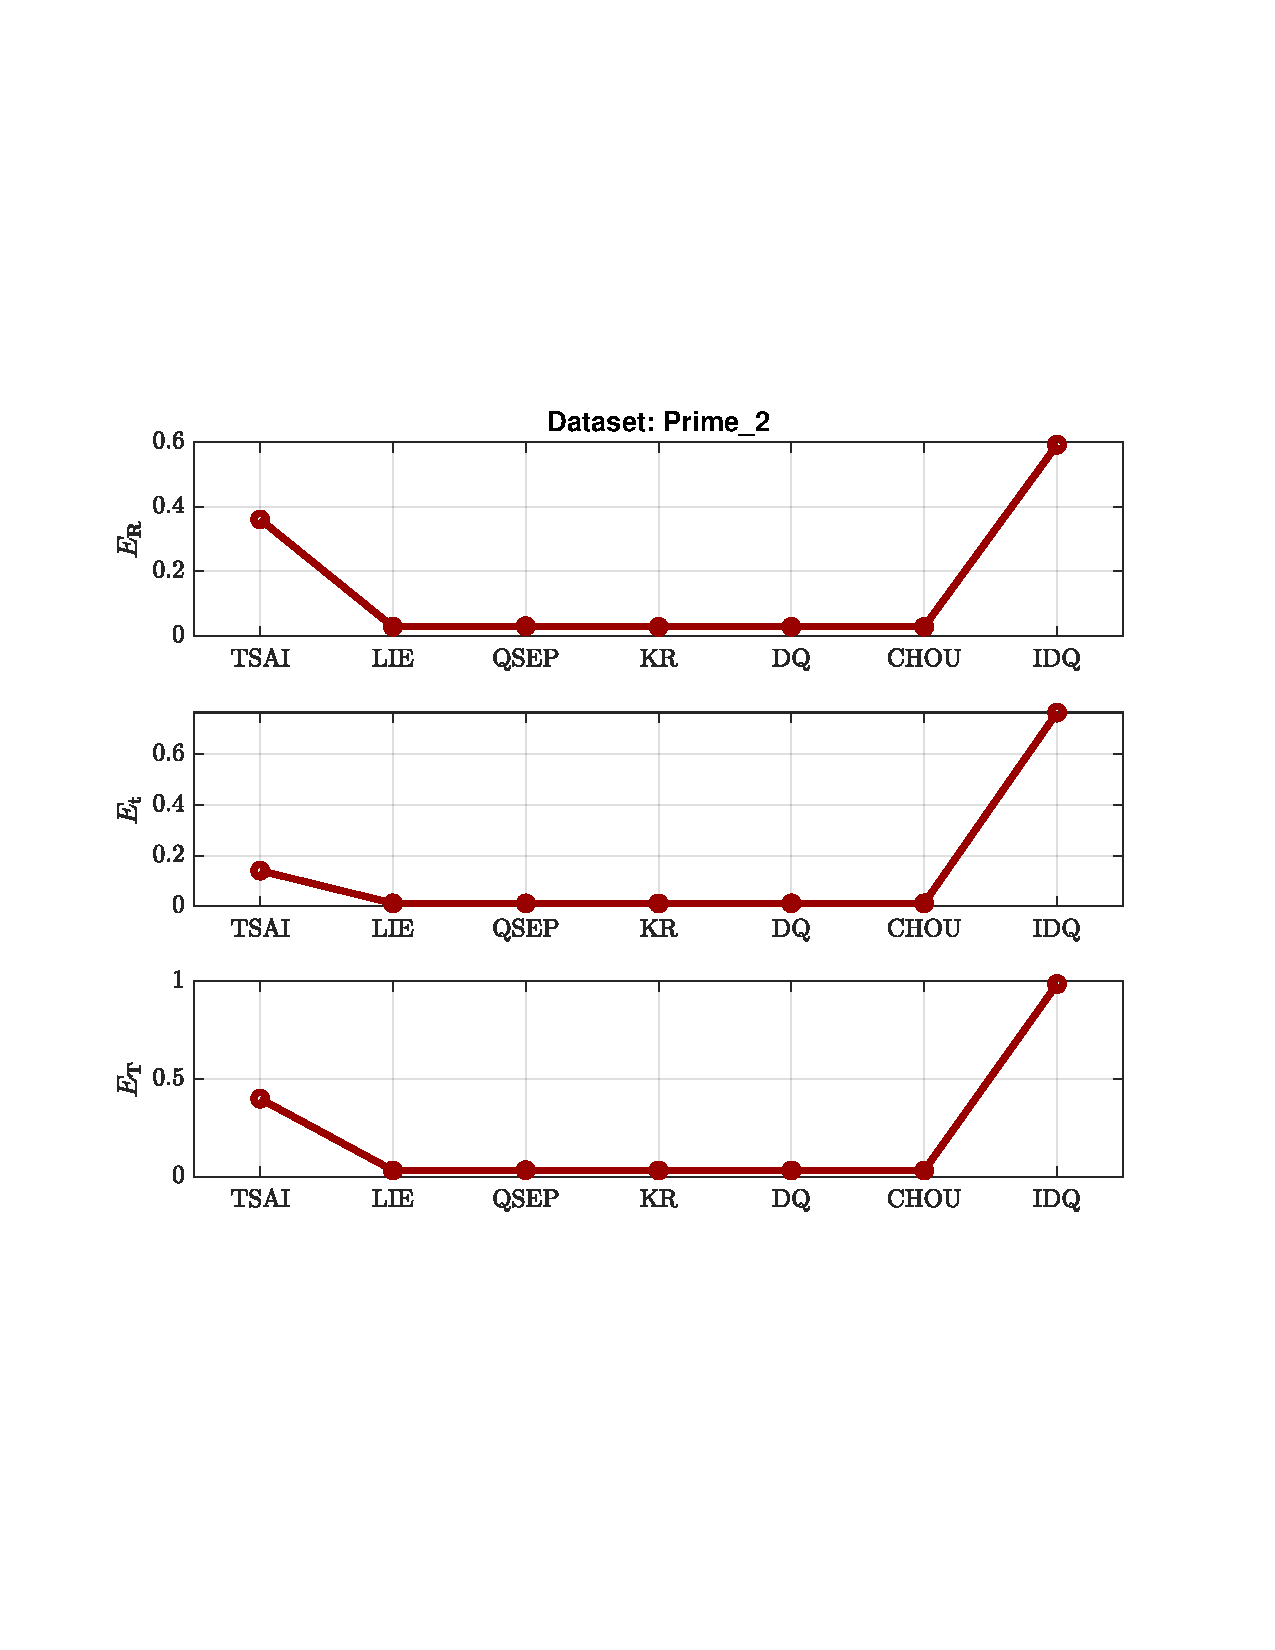
\includegraphics[scale=0.7]{./hand_eye_figures/real/Result_Prime_2}
\caption{Error plots for "\textbf{Primesense{\textunderscore}1}", "\textbf{Primesense{\textunderscore}2}" datasets denoted as \textbf{Prime{\textunderscore}1}, \textbf{Prime{\textunderscore}2}.}
\end{figure}

\begin{figure}
\centering
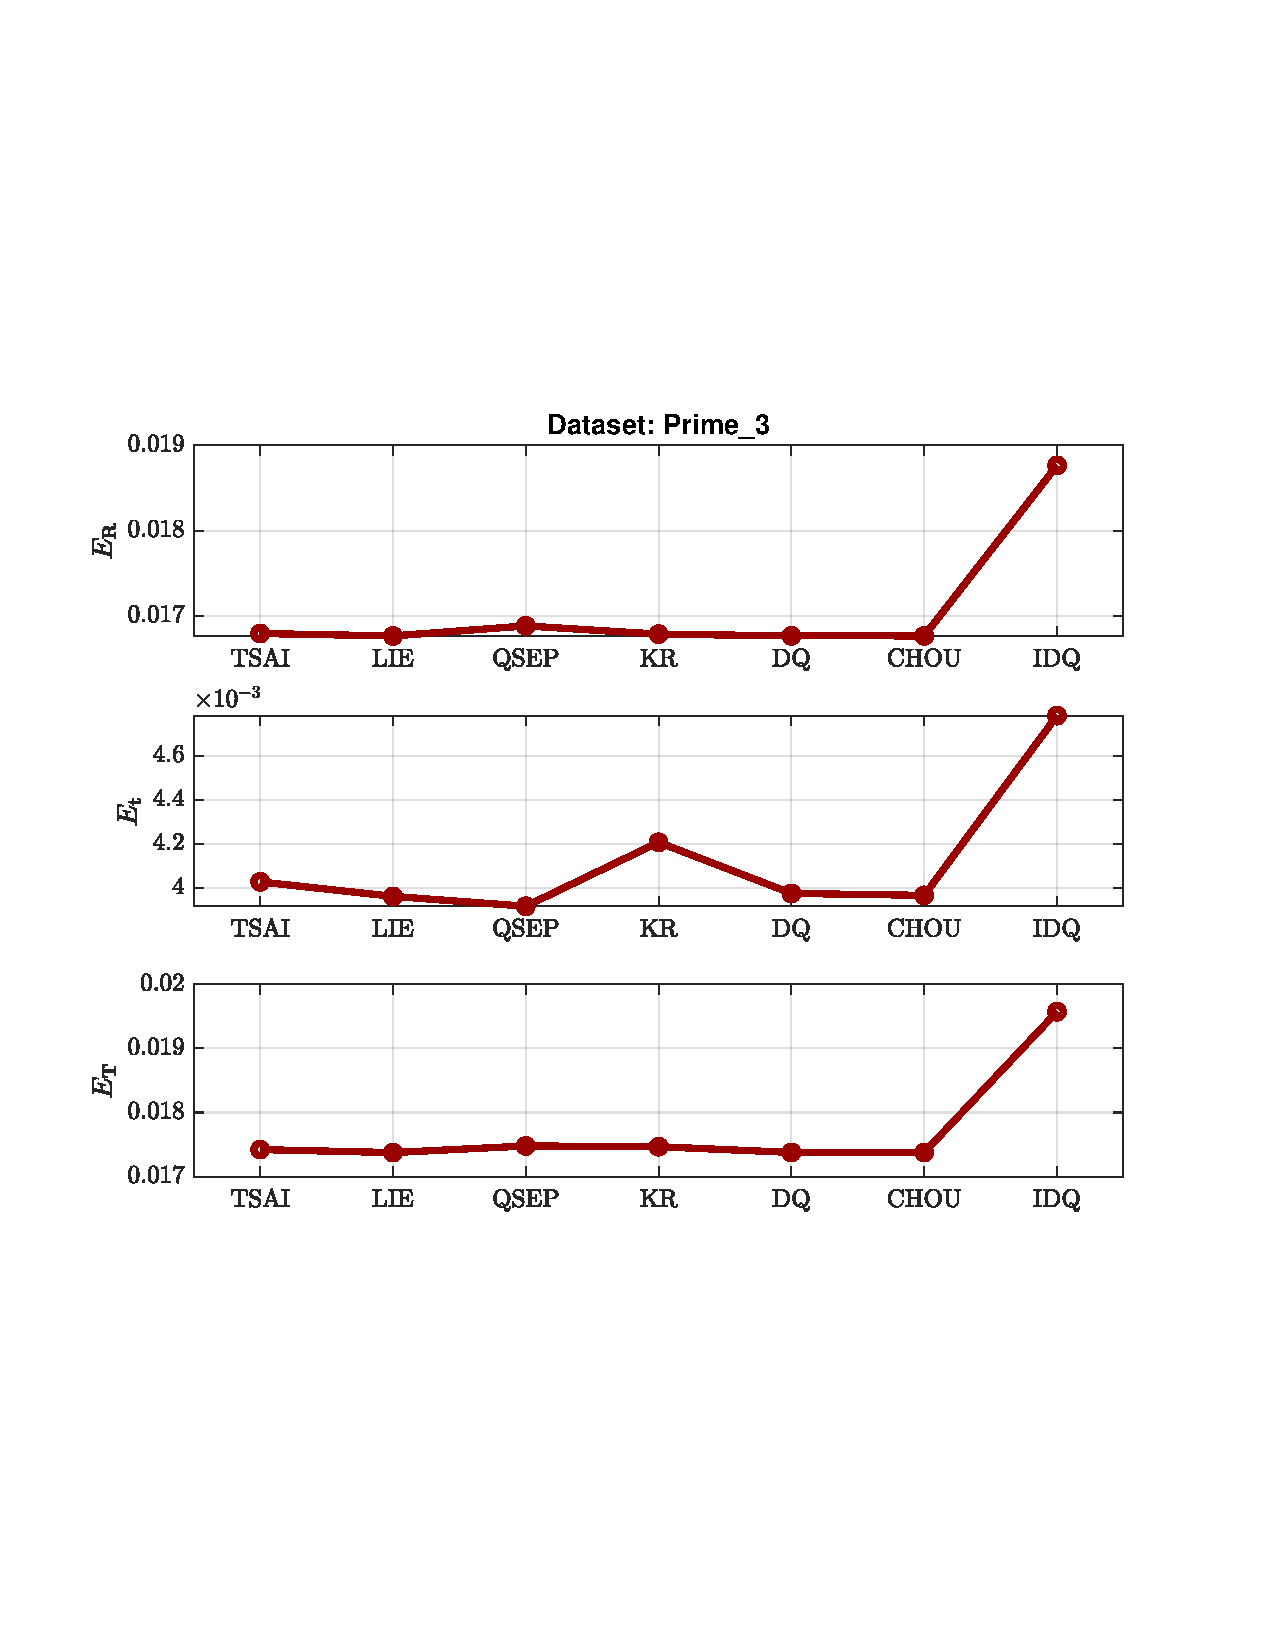
\includegraphics[scale=0.7]{./hand_eye_figures/real/Result_Prime_3}
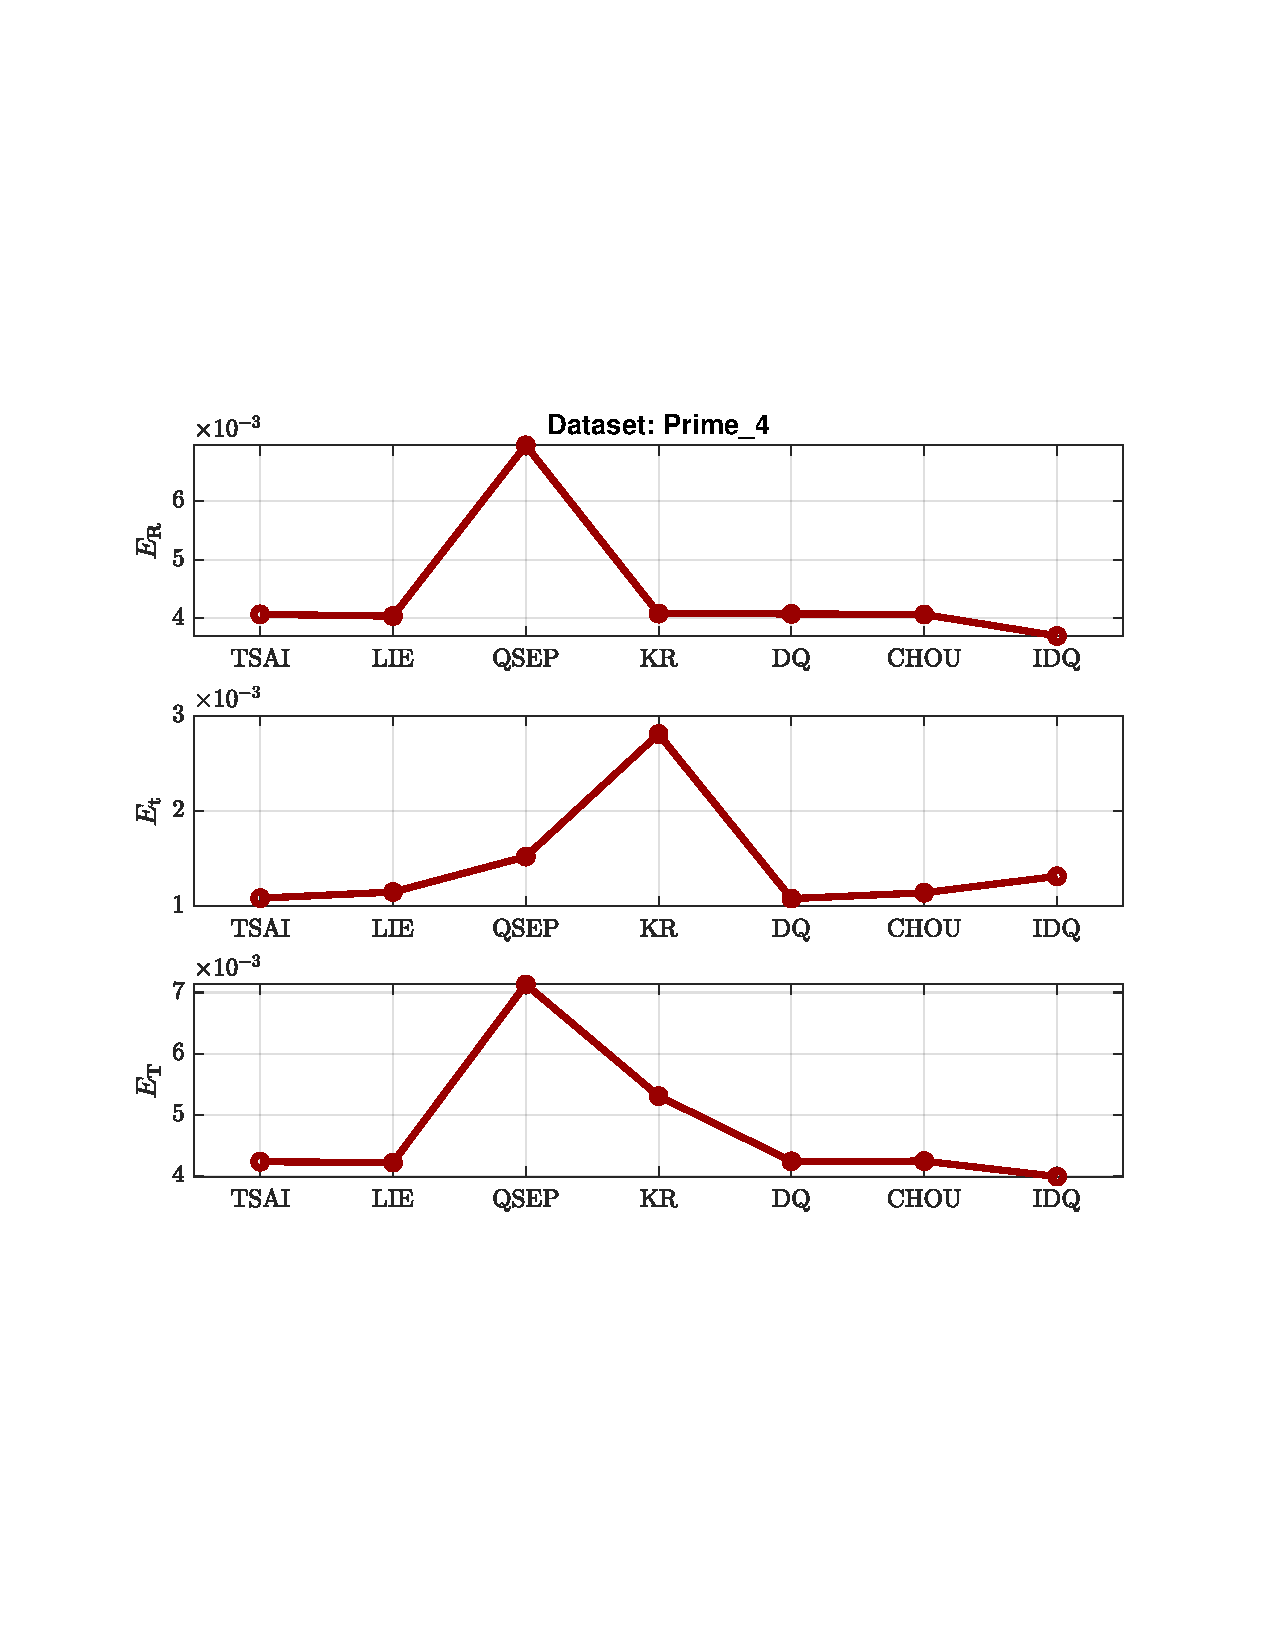
\includegraphics[scale=0.7]{./hand_eye_figures/real/Result_Prime_4}
\caption{Error plots for "\textbf{robot{\textunderscore}arm{\textunderscore}w{\textunderscore}color{\textunderscore}camera{\textunderscore}real}", "\textbf{robot{\textunderscore}arm{\textunderscore}w{\textunderscore}color{\textunderscore}camera{\textunderscore}sim}" datasets denoted as \textbf{Prime{\textunderscore}3}, \textbf{Prime{\textunderscore}4}.}
\end{figure}

\begin{figure}
\centering
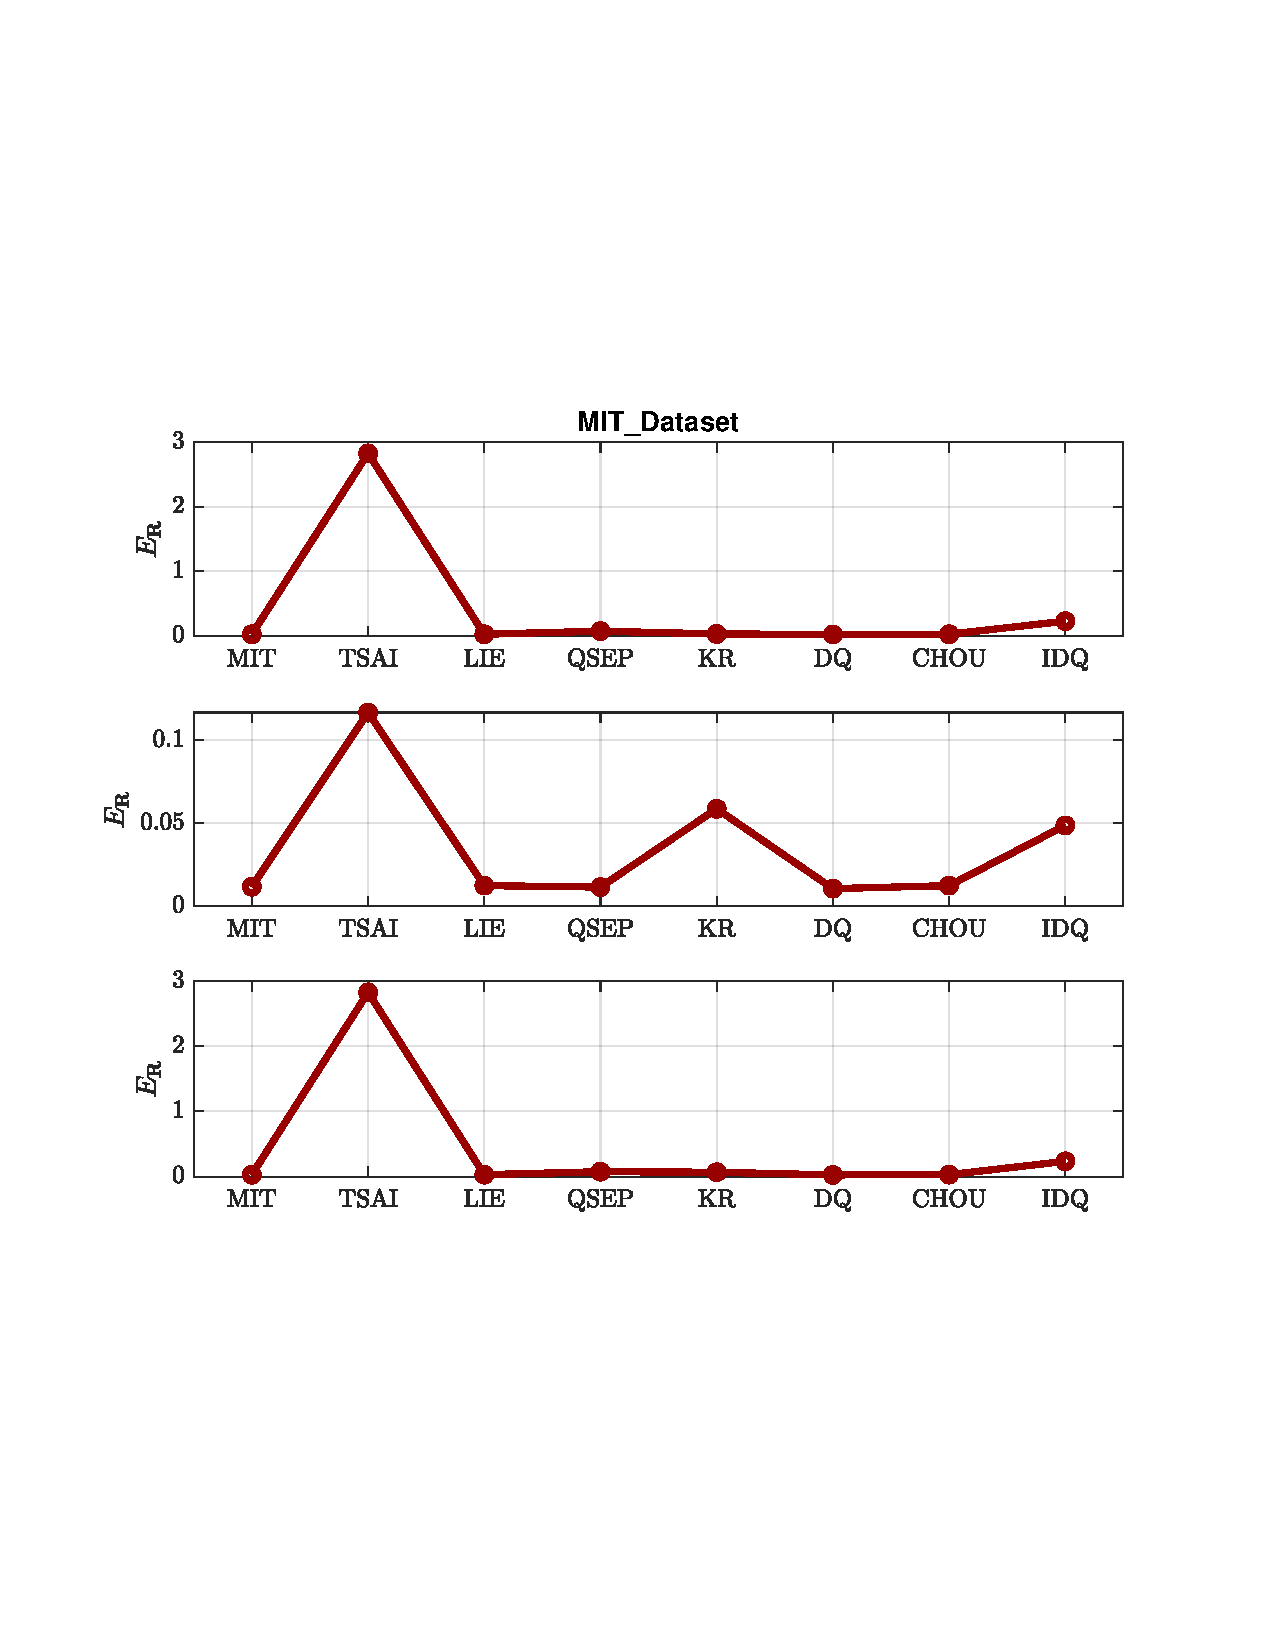
\includegraphics[scale=0.7]{./hand_eye_figures/real/Result_MIT_Dataset}
\caption{Error plots for \textbf{MIT dataset}.}
\end{figure}

\textcolor{red}{
From those figures, two methods (\textbf{TSAI}~\cite{tsai1989new} and \textbf{IDQ}~\cite{malti2010robust}) are filtered out because of their instabilities although they may outperform others in a certain dataset. Moreover, we can conclude that among those conventional methods, \textbf{LIE}~\cite{park1994robot} and \textbf{CHOU}~\cite{chou1991finding} are the most stable solutions compared with \textbf{QSEP}~\cite{horaud1995hand}. With regarding to the joint solutions, dual quaternion~\cite{daniilidis1999hand} is more stable than the Kronecker product solution~\cite{andreff1999line}}.

\begin{figure}
\centering
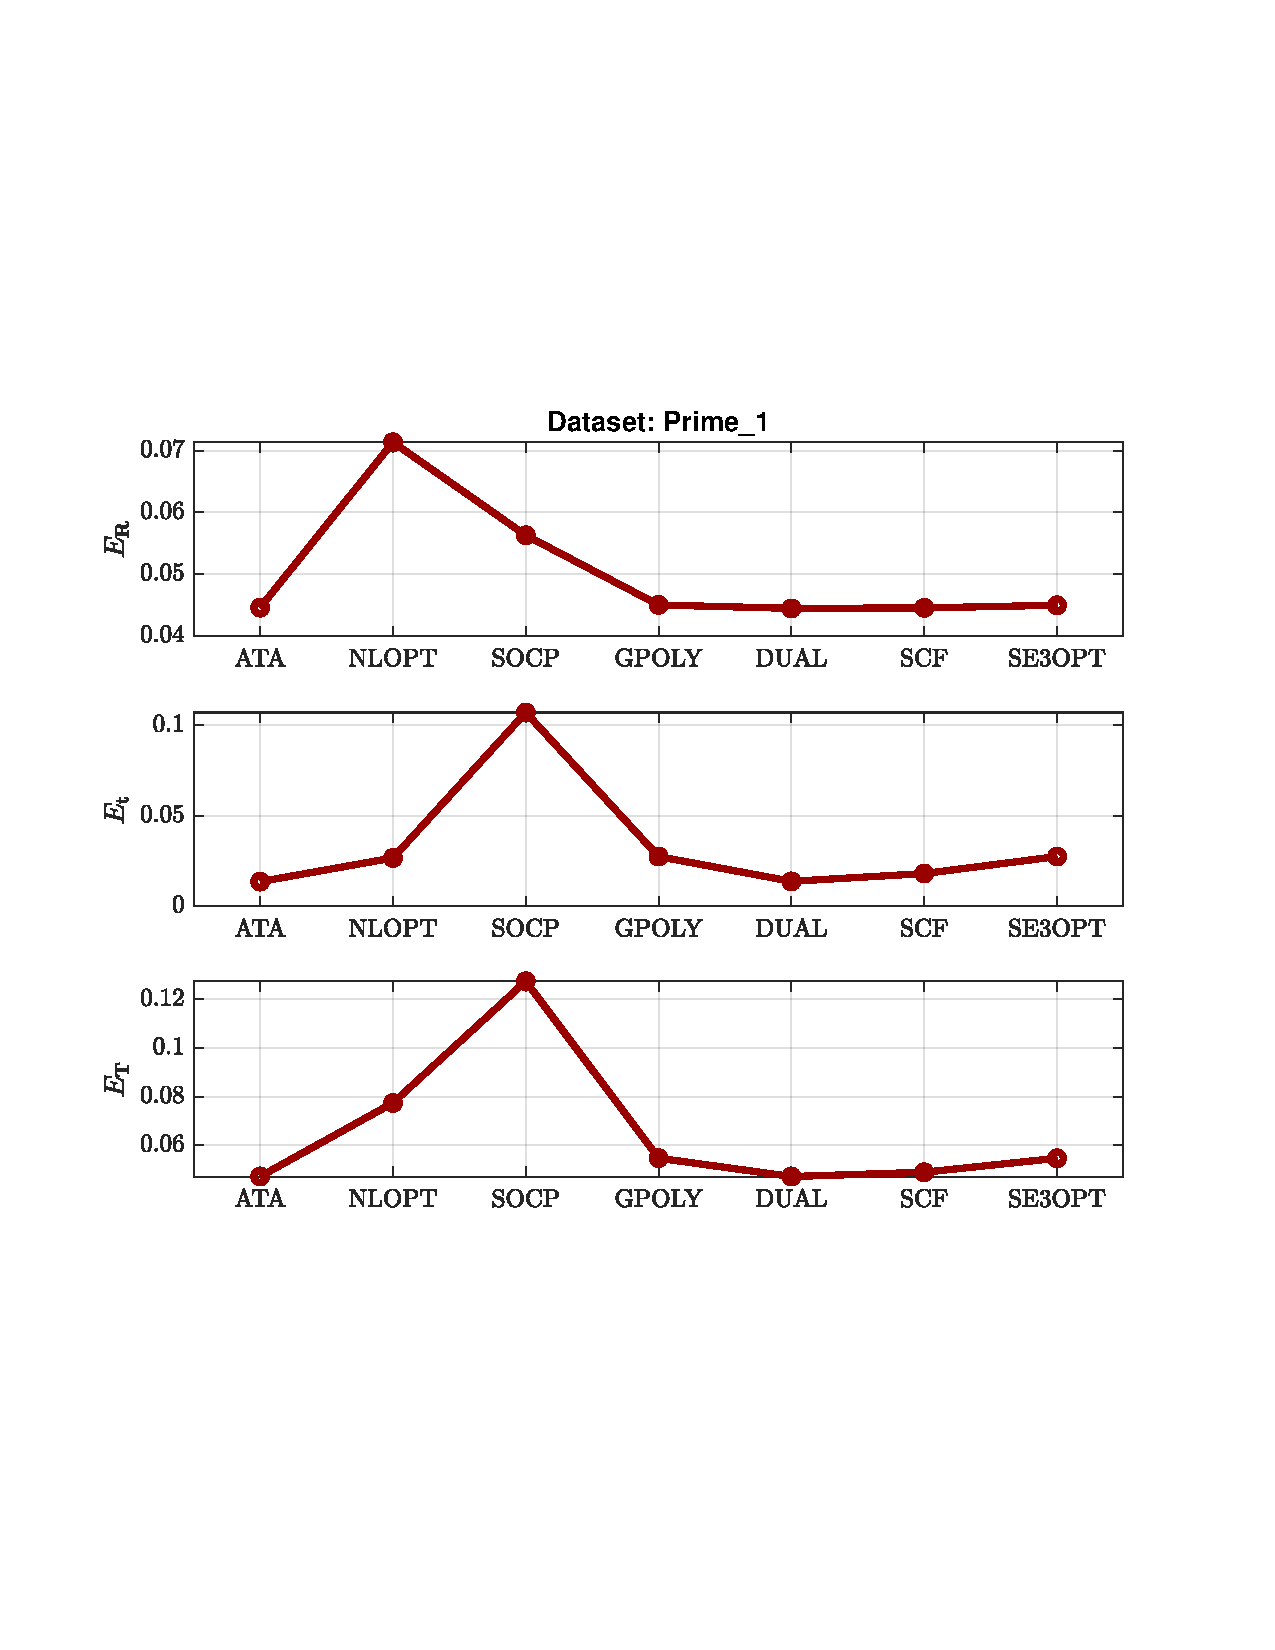
\includegraphics[scale=0.7]{./hand_eye_figures/real/adv_Result_Prime_1}
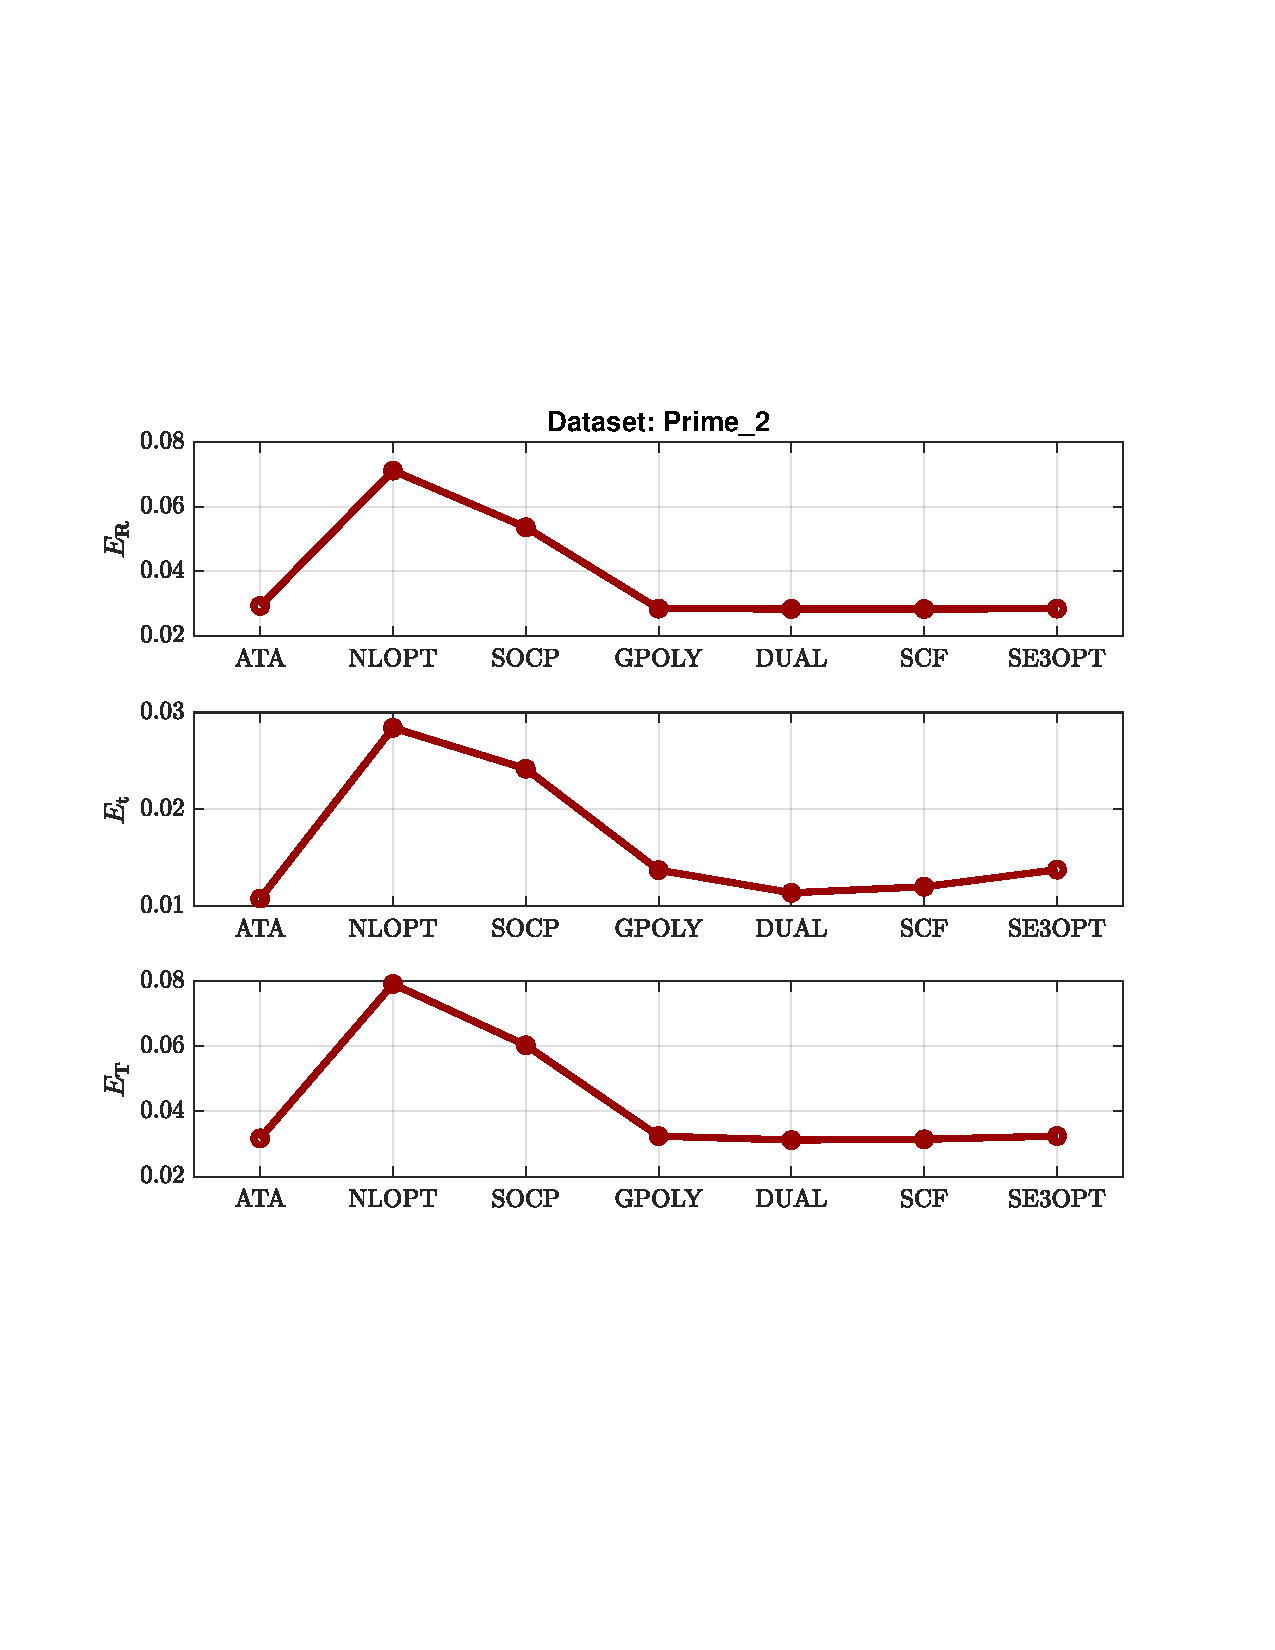
\includegraphics[scale=0.7]{./hand_eye_figures/real/adv_Result_Prime_2}
\caption{Error plots for "\textbf{Primesense{\textunderscore}1}", "\textbf{Primesense{\textunderscore}2}" datasets denoted as \textbf{Prime{\textunderscore}1}, \textbf{Prime{\textunderscore}2}.}
\end{figure}

\begin{figure}
\centering
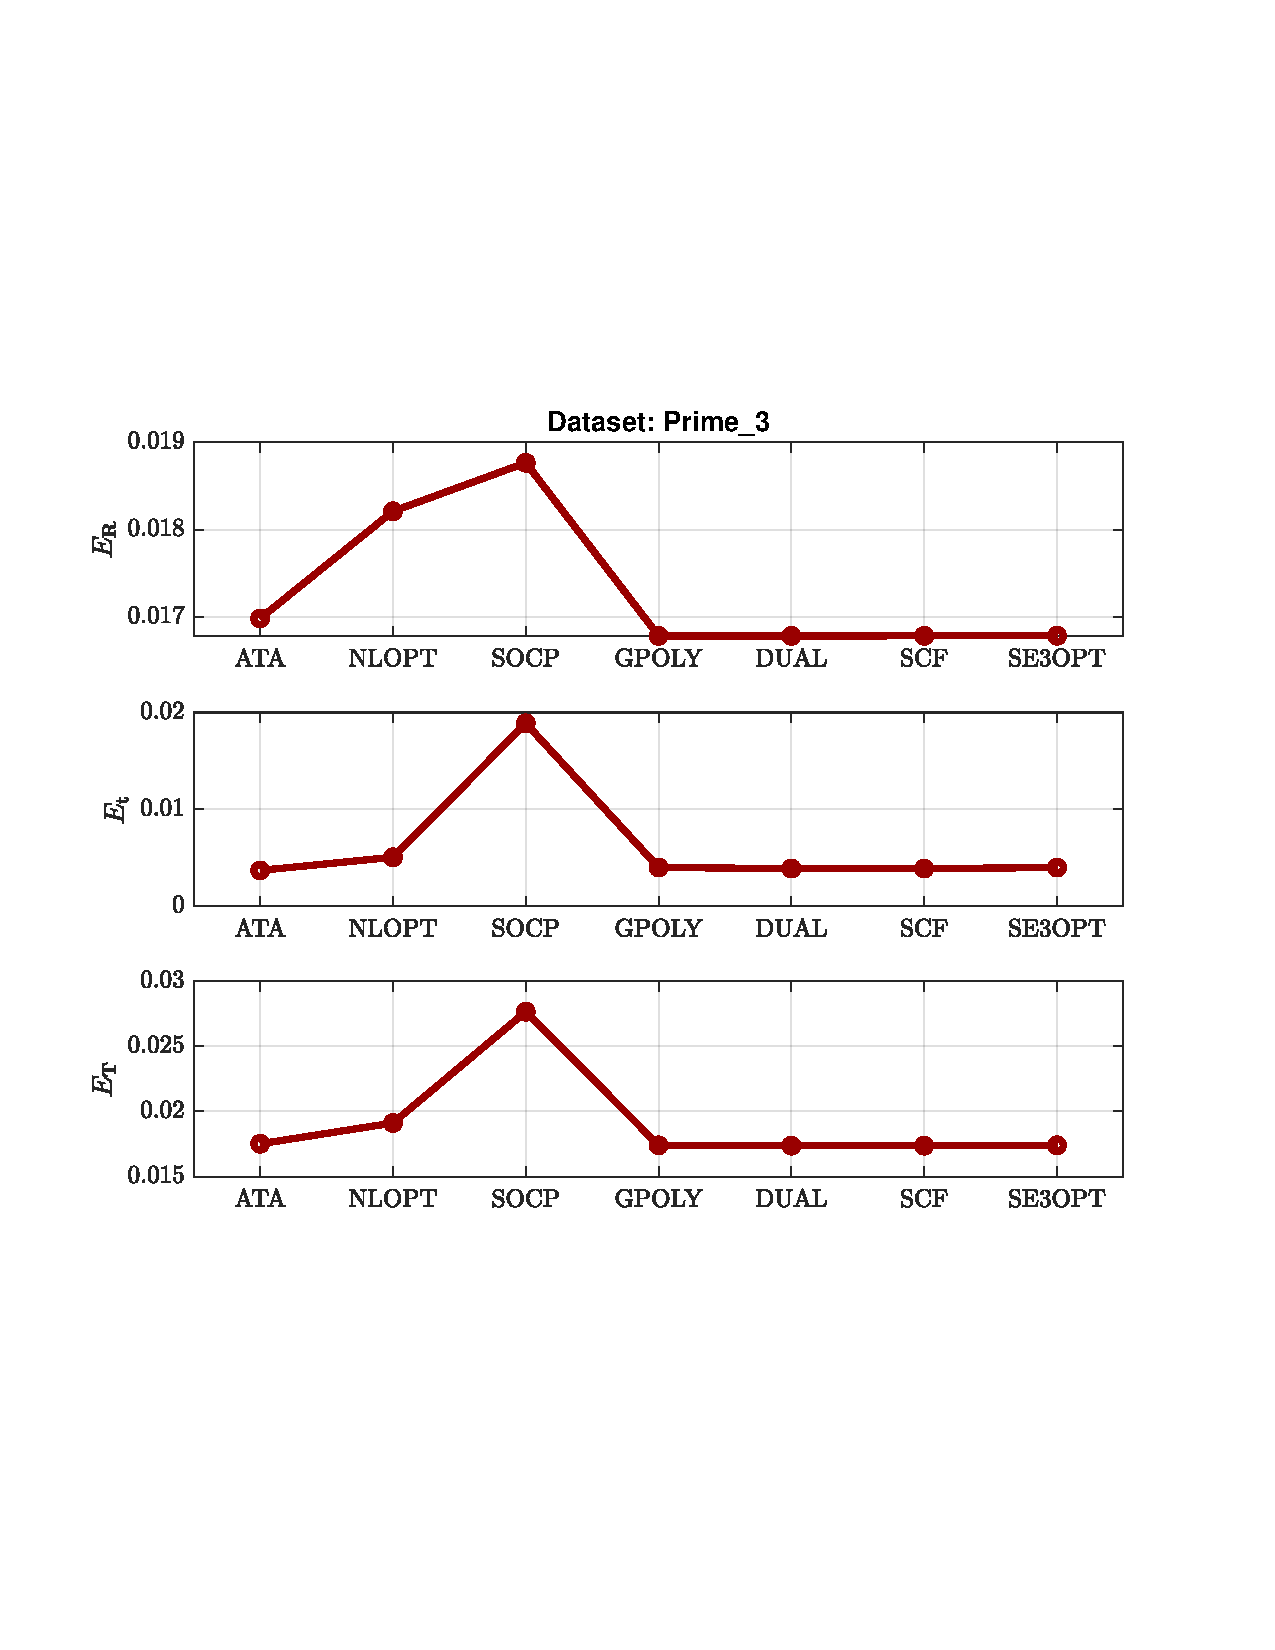
\includegraphics[scale=0.7]{./hand_eye_figures/real/adv_Result_Prime_3}
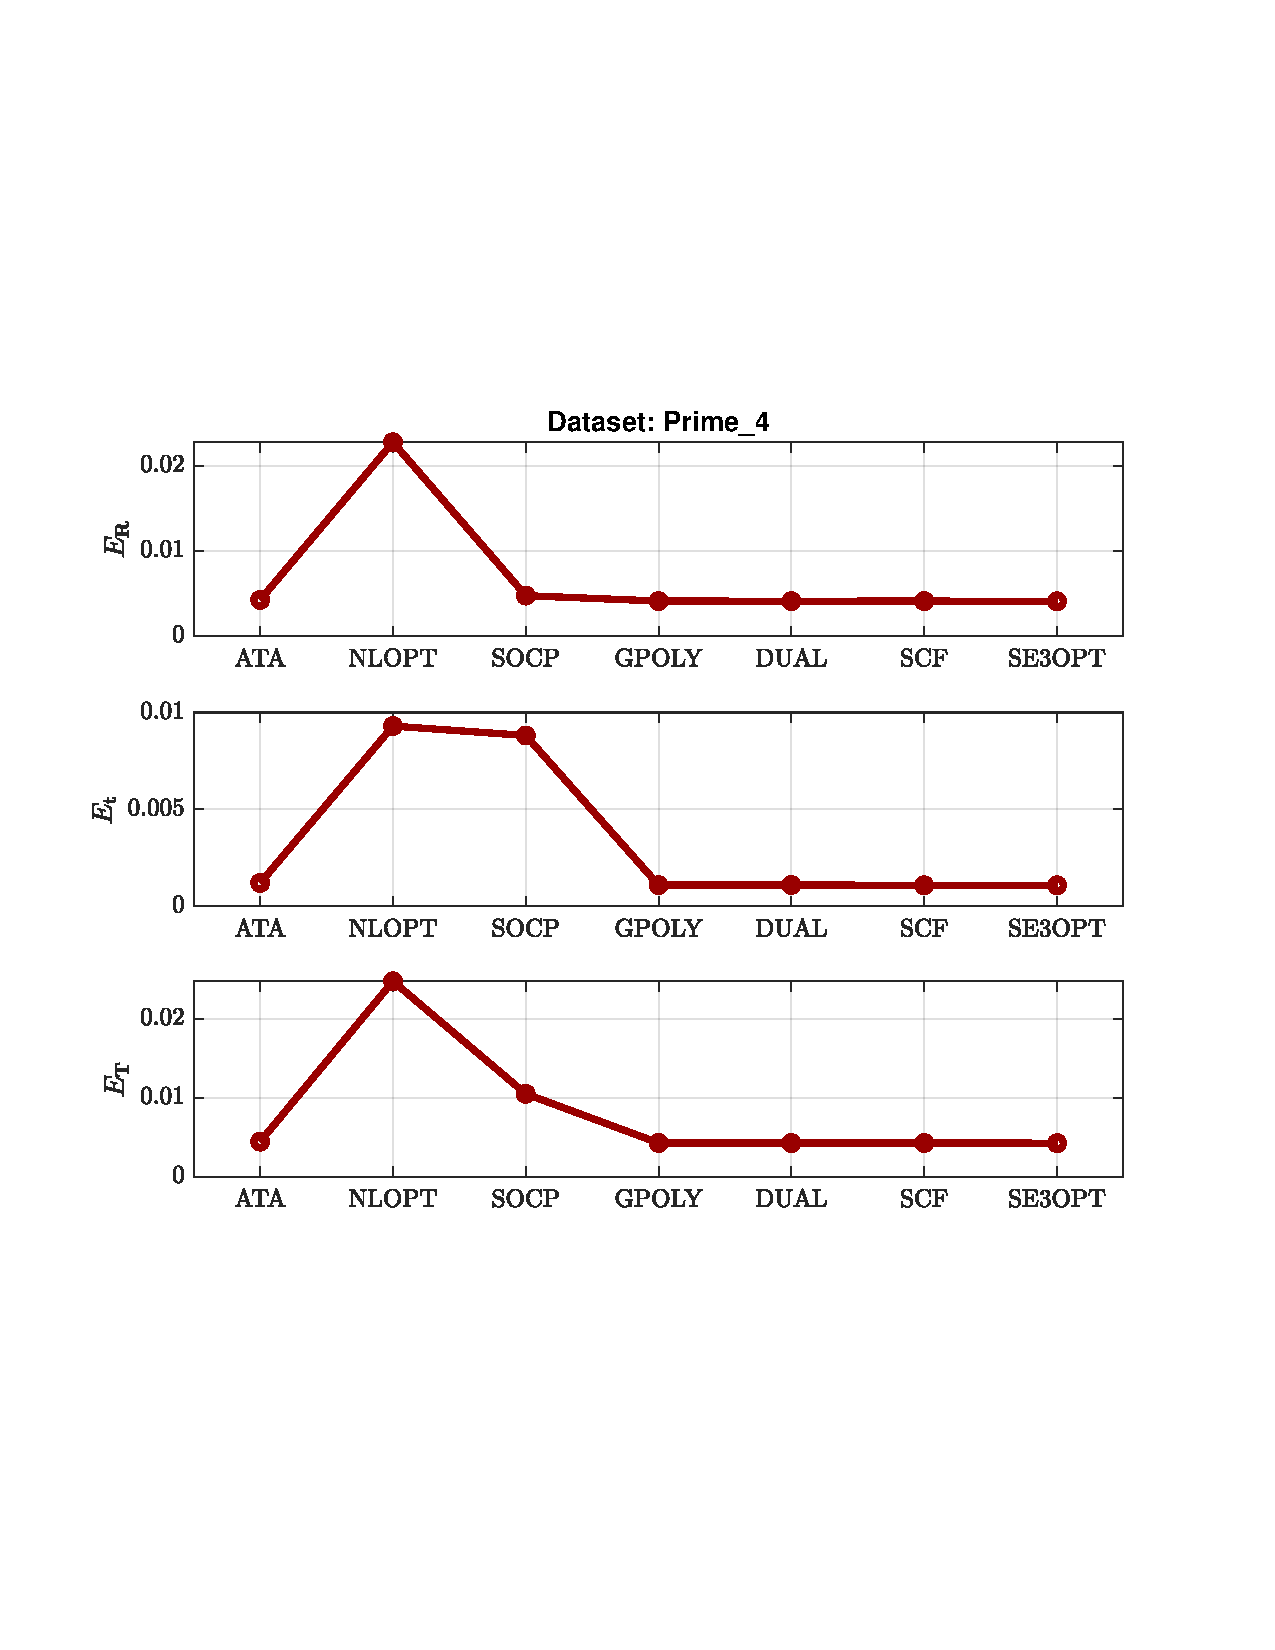
\includegraphics[scale=0.7]{./hand_eye_figures/real/adv_Result_Prime_4}
\caption{Error plots for "\textbf{robot{\textunderscore}arm{\textunderscore}w{\textunderscore}color{\textunderscore}camera{\textunderscore}real}", "\textbf{robot{\textunderscore}arm{\textunderscore}w{\textunderscore}color{\textunderscore}camera{\textunderscore}sim}" datasets denoted as \textbf{Prime{\textunderscore}3}, \textbf{Prime{\textunderscore}4}.}
\end{figure}

\begin{figure}
\centering
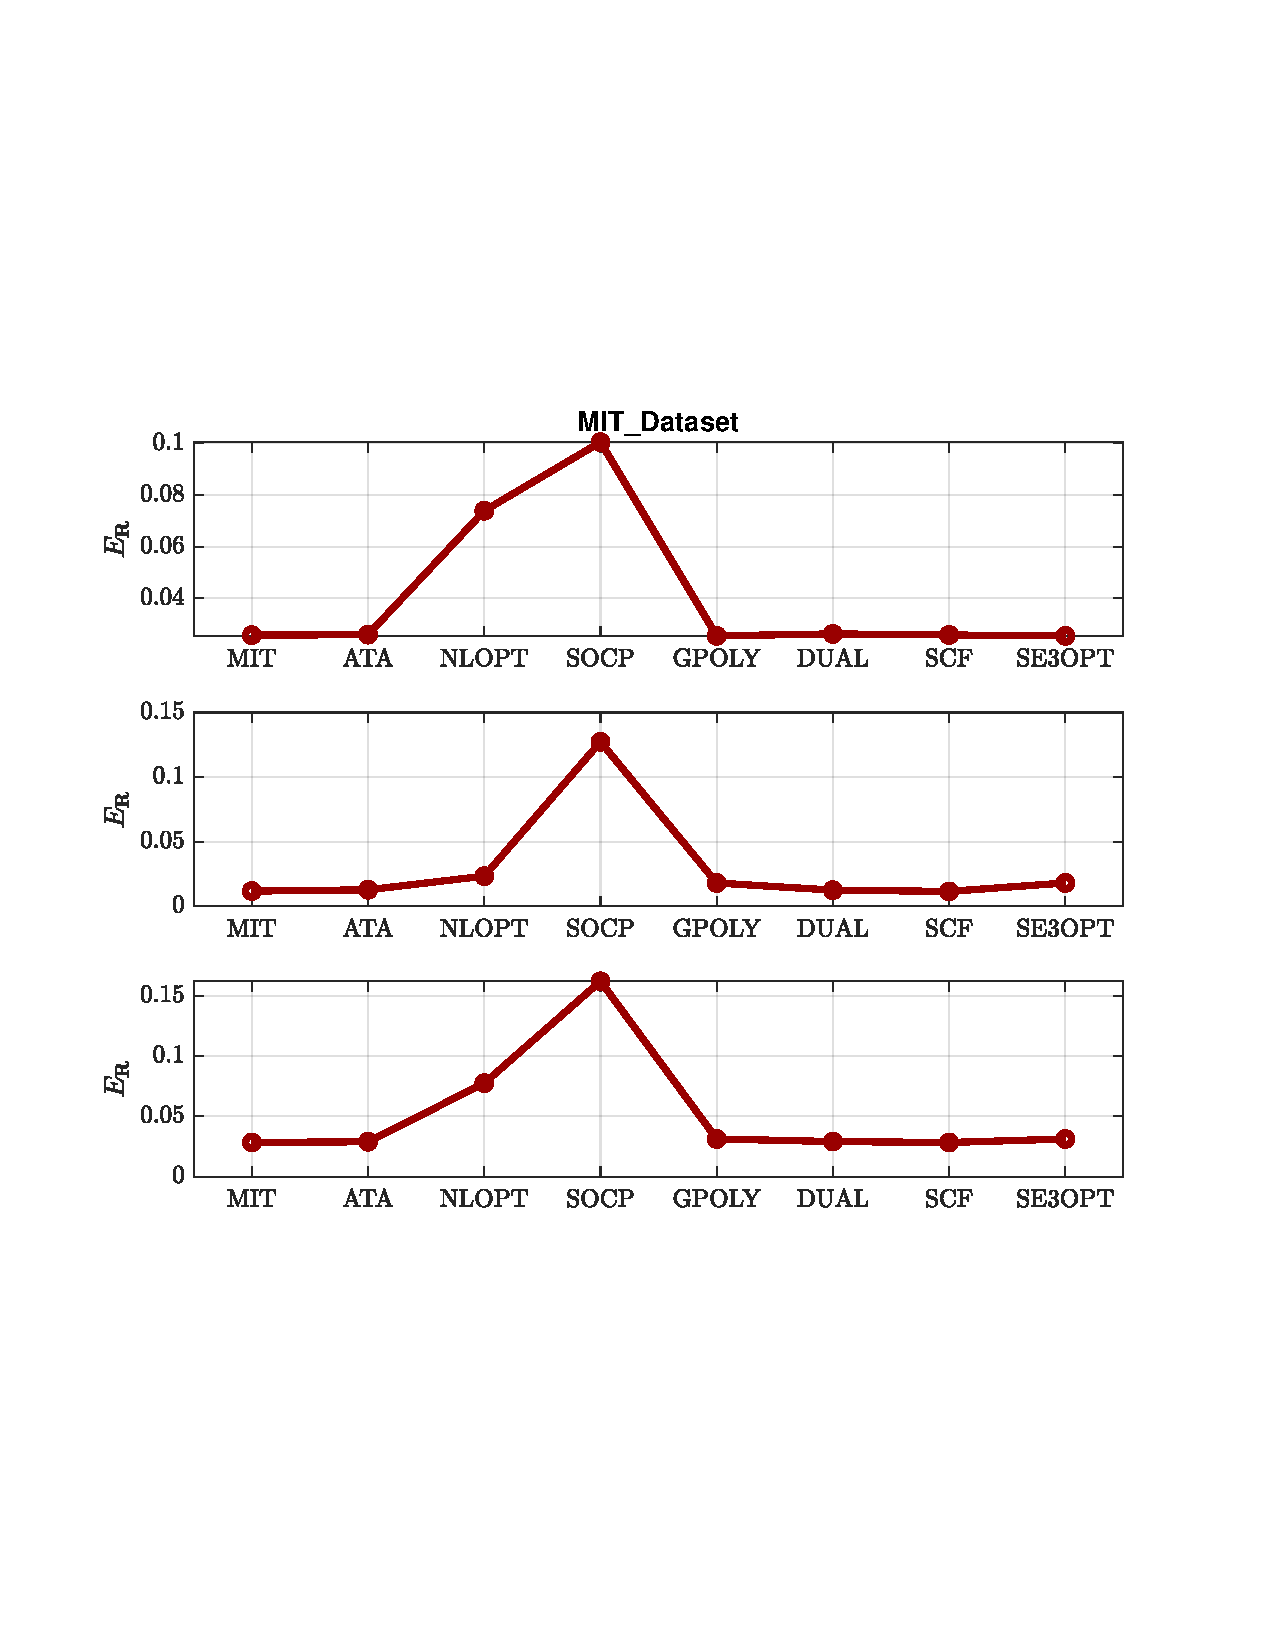
\includegraphics[scale=0.7]{./hand_eye_figures/real/adv_Result_MIT_Dataset}
\caption{Error plots for \textbf{MIT dataset}.}
\end{figure}

\textcolor{red}{
From those figures, two methods (\textbf{NLOPT}~\cite{horaud1995hand} and \textbf{SOCP}~\cite{zhao2011hand}) are filtered out because of their instabilities. } 

\begin{table}
\centering
\begin{tabular}{c|c|c|c}
$E_{\mathbf{R}}$ & $E_{\mathbf{t}}$ & $E_{\mathbf{T}}$ & $Runtime$\\ \hline
    $0.0258$ &   $0.0117$  &  $0.0283$ &  $3.7979$ \\ \hline
    $0.0310$ &   $0.0588$  &  $0.0665$ &  $0.0221$ \\ \hline
    $0.1005$ &   $0.1273$  &  $0.1622$ &  $5.8258$ \\ \hline
    $0.0260$ &   $0.0127$  &  $0.0289$ &  $0.5185$ \\ \hline
    $0.0255$ &   $0.0180$  &  $0.0312$ &  $1.6093$ \\ \hline
    $0.0263$ &   $0.0125$  &  $0.0291$ &  $0.9428$ \\ \hline
    $0.0257$ &   $0.0115$  &  $0.0282$ &  $0.3548$ \\ \hline                     
\hline
\end{tabular}
\end{table}

\chapter{Vision}
\section{Optical Flow}
\subsection{useful links}
\url{https://stackoverflow.com/questions/47465570/opencv-feature-matching-vs-optical-flow}.
\url{http://www.cad.zju.edu.cn/home/gfzhang/course/computational-photography/}.
\url{https://ags.cs.uni-kl.de/fileadmin/inf_ags/opt-ss12/lec05_opt.pdf}.
\url{http://people.csail.mit.edu/celiu/SIFTflow/ SIFT Flow}.
\url{https://www.reddit.com/r/computervision/comments/9n4o6p/optical_flow_vs_feature_matching_in_sparse_voslam/}.

\textcolor{blue}{So, basically speaking, optical flow is ok for small motion while feature matching can work with very large motion. From the comparison of running optical flow on the dataset captured by matrixvision and gopro, on mvision, although coarse-to-fine optical flow can track a certain number of features, but if I do a loop check (frame1 to frame2 and then backward from frame2 to frame1, and compare the result, theoretically, they should be the same or very small), I found very big error. However, on Gopro dataset, the optical flow works pretty well. The only difference is the FPS, gopro has 30 while mvision only has 10. So a small motion to gopro may mean a big motion to mvision. Another lesson learned from this experiment is the trade off between the tracking accuracy(winSize: small accurate) to the robustness (large window size tolerate large motion).}

\subsection{Tracking}
For optical flow, I use the LK tracker for constructing features correspondences. The lesson learned here is that the tracking results may contains severe wrong matches. So a loop fashion is favoured: 
\begin{itemize}
	\item do forward LK tracking from last frame to current frame;
	\item do backward LK tracking from current frame to last frame;
	\item check if the forward-backward feature point corresponds to the original feature point in the last frame by checking the relative distance; 
\end{itemize}
This can eliminate large number of wrong tracks.

\subsection{RANSAC}

\subsection{Homography}

\subsection{Fundamental Matrix}
The importance of applying normalization for fundamental matrix estimation was given in~\cite{hartley1995defence}.

\subsubsection{Composition}
\subsubsection{Computation}
\subsubsection{Tracking with special linear group}

\subsection{KD-Tree}
Since many computer vision tasks needs to find the correspondance and the low efficiency of brute-force search, KD tree is often used for boosting the searching procedure. Basically speaking, KD tree is a data structure which manages data by dividing the space into several sub-spaces. There are several stable and popular open source implementation of KD tree available on github:
\begin{itemize}
\item \textbf{nanoflann}\footnote{\url{https://github.com/jlblancoc/nanoflann}}
\item \textbf{FLANN}\footnote{\url{http://www.cs.ubc.ca/research/flann/}}: ANN for C, Matlab.
\item \textbf{kdtree}\footnote{\url{https://github.com/jtsiomb/kdtree}}: pure C implementation, I have once used this for path planning.
\end{itemize}
I have chosen \textbf{nanoflann} for KD tree implementation for program in \textsc{C/C++} and \textbf{FLANN} for ANN tree for program in \textsc{Matlab}.

Usage of \textbf{nanoflann}:
\begin{itemize}
\item create a kd-tree index: must specify distance template, data source type and dimension.
\item add points in chunks or build index;
\item 2 types of search: find nearest neighbours and find in radius;
\end{itemize}
SO3 is supported with quaternion and SO2 is supported with $\theta$.

\subsection{Feature \& Descriptor}
A fairly simple compare of commonly used features are given by\footnote{\url{https://marcosnietoblog.wordpress.com/}}.
I plan to try with \textbf{FAST}+\textbf{BRIEF} and \textbf{ORB}.
It could be very beneficial to read the source code of some feature detections and feature descriptions.

\subsection{Matching}
Normally, the matched correspondances would contain large number of wrong matches. The conventional methods which can mitigate this problem include:
\begin{enumerate}
	\item left-right check or even round check: match left to right then right to left, or previous to current and current to previous, and check if the corresponding point will round back to the original point. If not, consider a mismatch. This is robust, but time-consuming.
	\item uniqueness: find 2 best matches, only accept the match if the best score if significantly smaller than the second best score.
	\item na\"{\i}ve method including compute the mean and standard deviation of the distance and then filter out matches whose distance is beyond a threshold. This can also be done to compute mean and standard deviation of the displacement between two frames.
	\item use epipolar constraint or use homography constraint: the idea is to compute the fundamental or homography matrix and then corresponding distances. Filter out matches whose distance is over a threshold. This should be the most time consuming approach.
\end{enumerate}
\textcolor{blue}{It is better to see if some one can test this}.


\chapter{Complete Solution}
1. ~\cite{schmidt2005calibration}.

\bibliography{hand_eye_calibration} 
\bibliographystyle{ieeetr}

\end{document}